\everymath{\displaystyle}
\documentclass{beamer}
% \documentclass[handout]{beamer}

%\usepackage[pdftex]{color,graphicx}
\usepackage{amsmath,amssymb,amsfonts}

\mode<presentation>
{
  % \usetheme{Darmstadt}
  % \usetheme[hideothersubsections]{Hannover}
  % \usetheme[hideothersubsections]{Goettingen}
  \usetheme[hideothersubsections, right]{Berkeley}

  \usecolortheme{seahorse}
  % \usecolortheme{dolphin}
  \usecolortheme{rose}
  % \usecolortheme{orchid}

  \useinnertheme[shadow]{rounded}

  % \setbeamercovered{transparent}
  \setbeamercovered{invisible}
  % or whatever (possibly just delete it)
}

\mode<handout>{
  \setbeamercolor{background canvas}{bg=black!5}
  \usepackage{pgfpages}
  \pgfpagesuselayout{4 on 1}[a4paper,border shrink=5mm, landscape]
}

\usepackage[brazilian]{babel}
% or whatever

% \usepackage[latin1]{inputenc}
\usepackage[utf8]{inputenc}
% or whatever

\usepackage{times}
%\usepackage[T1]{fontenc}
% Or whatever. Note that the encoding and the font should match. If T1
% does not look nice, try deleting the line with the fontenc.

\title%[] % (optional, use only with long paper titles)
{Tópicos em Regressão Logística}

\subtitle
{Modelos com desfecho categórico binário} % (optional)

\author%[] % (optional, use only with lots of authors)
{Felipe Figueiredo}% \and S.~Another\inst{2}}
% - Use the \inst{?} command only if the authors have different
%   affiliation.

\institute[INTO] % (optional, but mostly needed)
{Instituto Nacional de Traumatologia e Ortopedia
}
  % \inst{1}%
  % Department of Computer Science\\
  % University of Somewhere
  % \and
  % \inst{2}%
  % Department of Theoretical Philosophy\\
  % University of Elsewhere}
% - Use the \inst command only if there are several affiliations.
% - Keep it simple, no one is interested in your street address.

\date%[] % (optional)
{}

% \subject{Talks}
% This is only inserted into the PDF information catalog. Can be left
% out. 



% If you have a file called "university-logo-filename.xxx", where xxx
% is a graphic format that can be processed by latex or pdflatex,
% resp., then you can add a logo as follows:

\pgfdeclareimage[height=1.6cm]{university-logo}{../logo}
\logo{\pgfuseimage{university-logo}}



% Delete this, if you do not want the table of contents to pop up at
% the beginning of each subsection:
\AtBeginSubsection[]
%\AtBeginSection[]
{
  \begin{frame}<beamer>{Sumário}
    \tableofcontents[currentsection,currentsubsection]
  \end{frame}
}


% If you wish to uncover everything in a step-wise fashion, uncomment
% the following command: 

% \beamerdefaultoverlayspecification{<+->}

\usepackage[normalem]{ulem}

\begin{document}

\begin{frame}
  \titlepage
\end{frame}

\begin{frame}{Sumário}
  \tableofcontents
  % You might wish to add the option [pausesections]
\end{frame}


%% Template
% \section{}

% \subsection{}

% \begin{frame}{}
%   \begin{itemize}
%   \item 
%   \end{itemize}
% \end{frame}

% \begin{frame}
%   \begin{columns}
%     \begin{column}{5cm}
%     \end{column}
%     \begin{column}{5cm}
%     \end{column}
%   \end{columns}
% \end{frame}

% \begin{frame}{}
%   \includegraphics[height=0.4\textheight]{file1}
%   \includegraphics[height=0.4\textheight]{file2}
%   \includegraphics[height=0.4\textheight]{file3}
%   \begin{figure}
%     \caption{}
%   \end{figure}
% \end{frame}

% \begin{frame}{}
%   \begin{definition}
%   \end{definition}
%   \begin{example}
%   \end{example}
%   \begin{block}{Exercício}
%   \end{block}
% \end{frame}

% \section{Discussão da aula passada}

% \subsection{Discussão da aula passada}

\begin{frame}{\scriptsize Discussão da aula passada}
  \begin{block}{}
    Discussão da leitura obrigatória da aula passada
  \end{block}
\end{frame}

\section{Regressão Linear Múltipla}

\subsection{Regressão Linear Múltipla}

\begin{frame}{\scriptsize }
  \begin{center}
    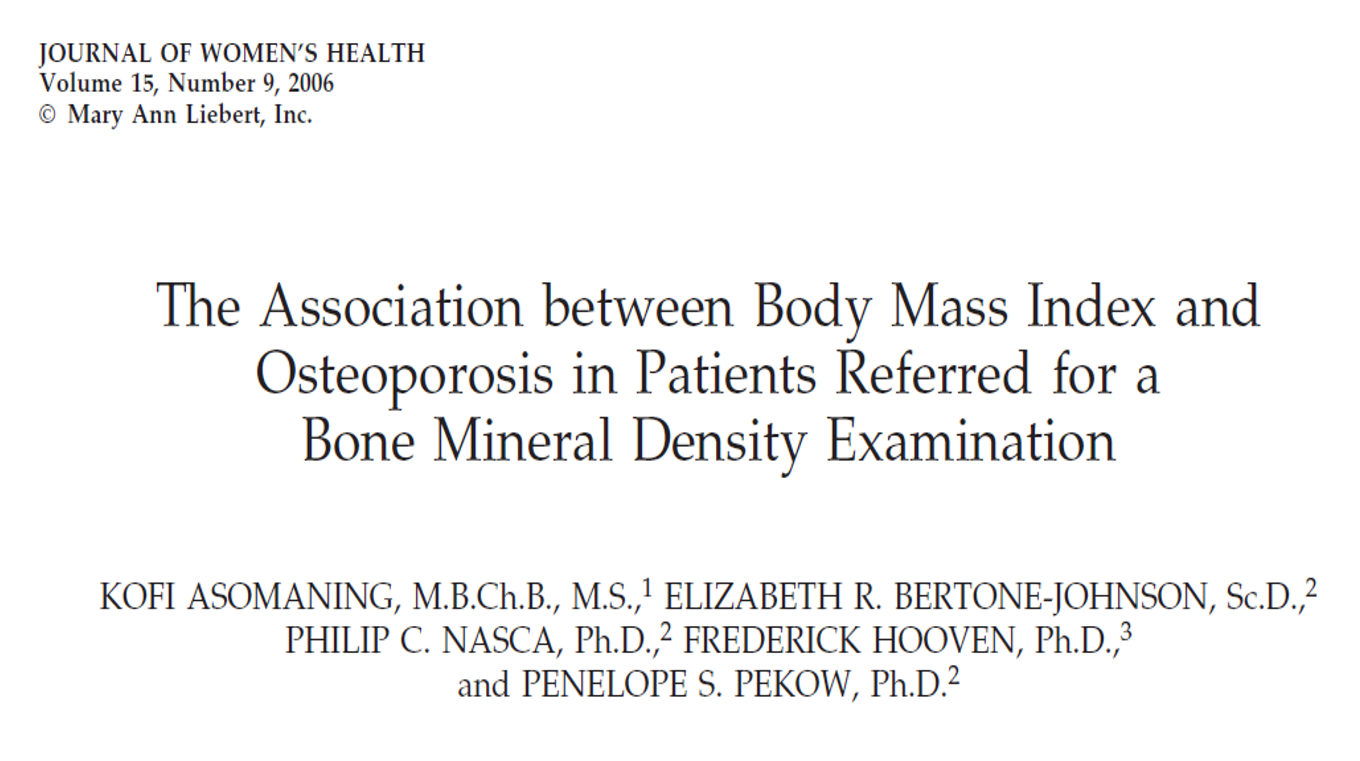
\includegraphics[width=\textwidth]{Cap18-19/bmi-bmd-title}
  \end{center}
\end{frame}

\begin{frame}{\scriptsize }
  \begin{center}
    Hoje vamos interpretar os resultados do abstract
  \end{center}
\end{frame}

\begin{frame}{\scriptsize }
  \begin{center}
    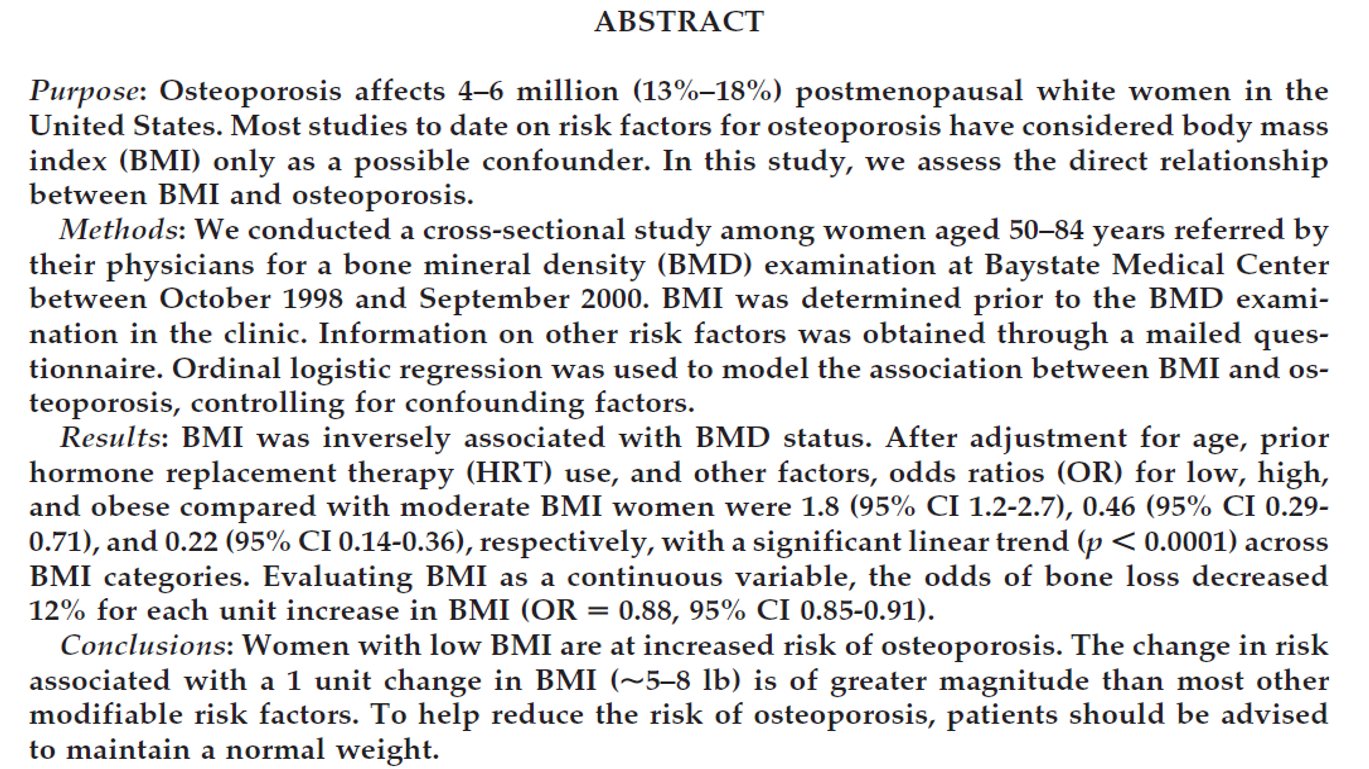
\includegraphics[width=1.175\textwidth]{Cap18-19/bmi-bmd-abstract}
  \end{center}
\end{frame}

\begin{frame}{\scriptsize }
  \begin{exampleblock}{Enunciado 1}
    \footnotesize
    Os pesquisadores querem investigar se o grupo etnicidade das participantes tem algum efeito detectável na associação entre
    a densidade mineral óssea (BMD) e o índice de massa corpórea (BMI).

    \bigskip
    \begin{exampleblock}{}
    \footnotesize
    Para isto selecionaram 100 mulheres brancas e 100 mulheres pardas, de meia idade.
    Mensuraram a BMD e calcularam o BMI delas.
  \end{exampleblock}

  \end{exampleblock}
\end{frame}

\begin{frame}{\scriptsize Modelo 1}
  \begin{center}
    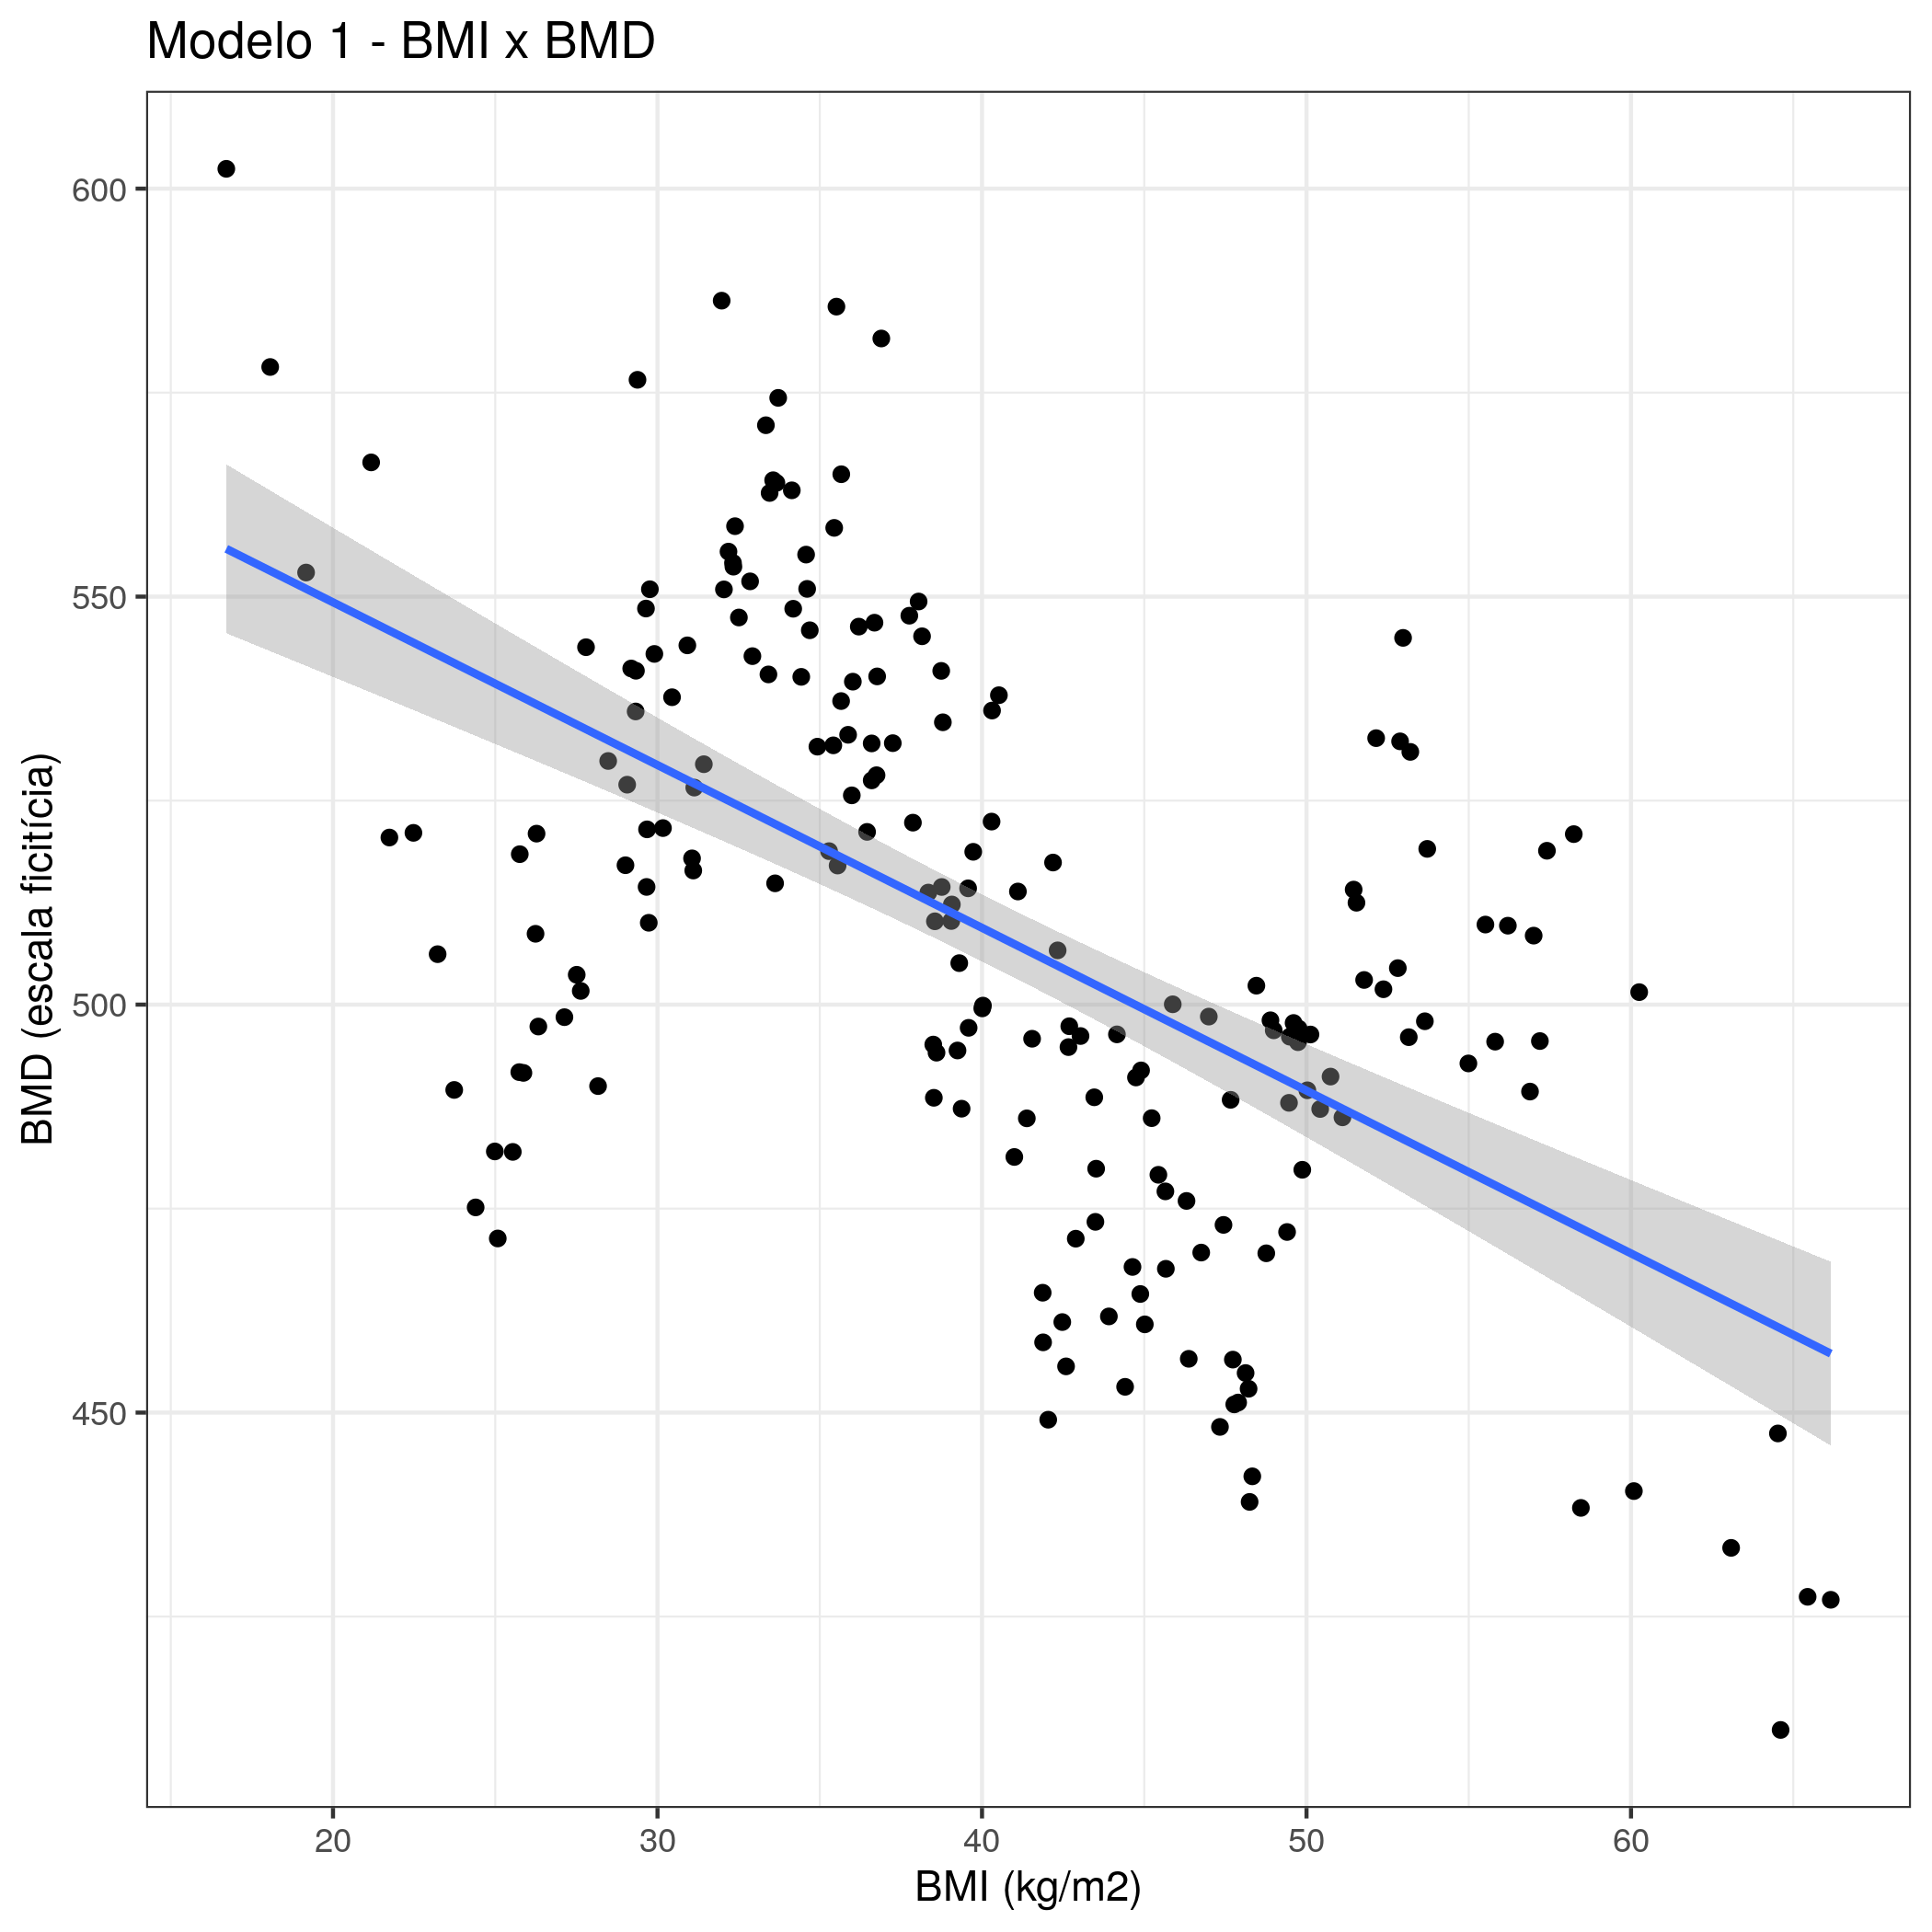
\includegraphics[height=.9\textheight]{Cap31-32/pratica-rlm1}
  \end{center}
\end{frame}

\begin{frame}{\scriptsize Quais são as variáveis?}
  \begin{itemize}
    \footnotesize
  \item Dependente: BMD (contínua)
  \item Independente: BMI (contínua)
  \end{itemize}
  \vfill
  \begin{block}{Esta relação pode ser expressa como}
    \footnotesize
    \begin{displaymath}
      \text{BMD} \sim \text{BMI}
    \end{displaymath}
  \end{block}
\end{frame}

\begin{frame}{\scriptsize Componentes do modelo 1}
  \begin{block}{\footnotesize Versão simplificada (apenas variáveis)}
    \footnotesize
    \begin{displaymath}
      \text{BMD} \sim \text{BMI}
    \end{displaymath}
  \end{block}
  \bigskip
  \bigskip
  \begin{block}{Modelo completo}
    \footnotesize
    \begin{displaymath}
      \text{BMD} =\beta_0 + \beta_1 \text{(BMI)} + \varepsilon
    \end{displaymath}
  \end{block}
  \vfill
  \footnotesize
  Hipótese: $\varepsilon$ é um erro aleatório \footnote{\scriptsize residual -- não é explicado pela relação entre as variáveis do modelo} normalmente distribuído e centrado em zero -- a incerteza que não pode ser controlada.
\end{frame}

\begin{frame}[fragile]{\scriptsize }
  \begin{center}
    \begin{exampleblock}{Modelo 1}
      \tiny
\begin{verbatim}
Residuals:
    Min      1Q  Median      3Q     Max 
-50.770 -14.570  -2.449  14.357  58.778 

Coefficients:
            Estimate Std. Error t value Pr(>|t|)    
(Intercept) 607.3708     5.9857  101.47   <2e-16 ***
BMI          -1.9848     0.1444  -13.75   <2e-16 ***
---
Signif. codes:  0 ‘***’ 0.001 ‘**’ 0.01 ‘*’ 0.05 ‘.’ 0.1 ‘ ’ 1

Residual standard error: 20.71 on 198 degrees of freedom
Multiple R-squared:  0.4884,	Adjusted R-squared:  0.4858 
F-statistic:   189 on 1 and 198 DF,  p-value: < 2.2e-16
\end{verbatim}
    \end{exampleblock}
  \begin{exampleblock}{Modelo 1 completo}
    \footnotesize
    \begin{displaymath}
      \text{BMD} =607.37 -1.98 \times\text{BMI}
    \end{displaymath}
  \end{exampleblock}
  \end{center}
\end{frame}

\begin{frame}{\scriptsize Modelo 1}
  \begin{center}
    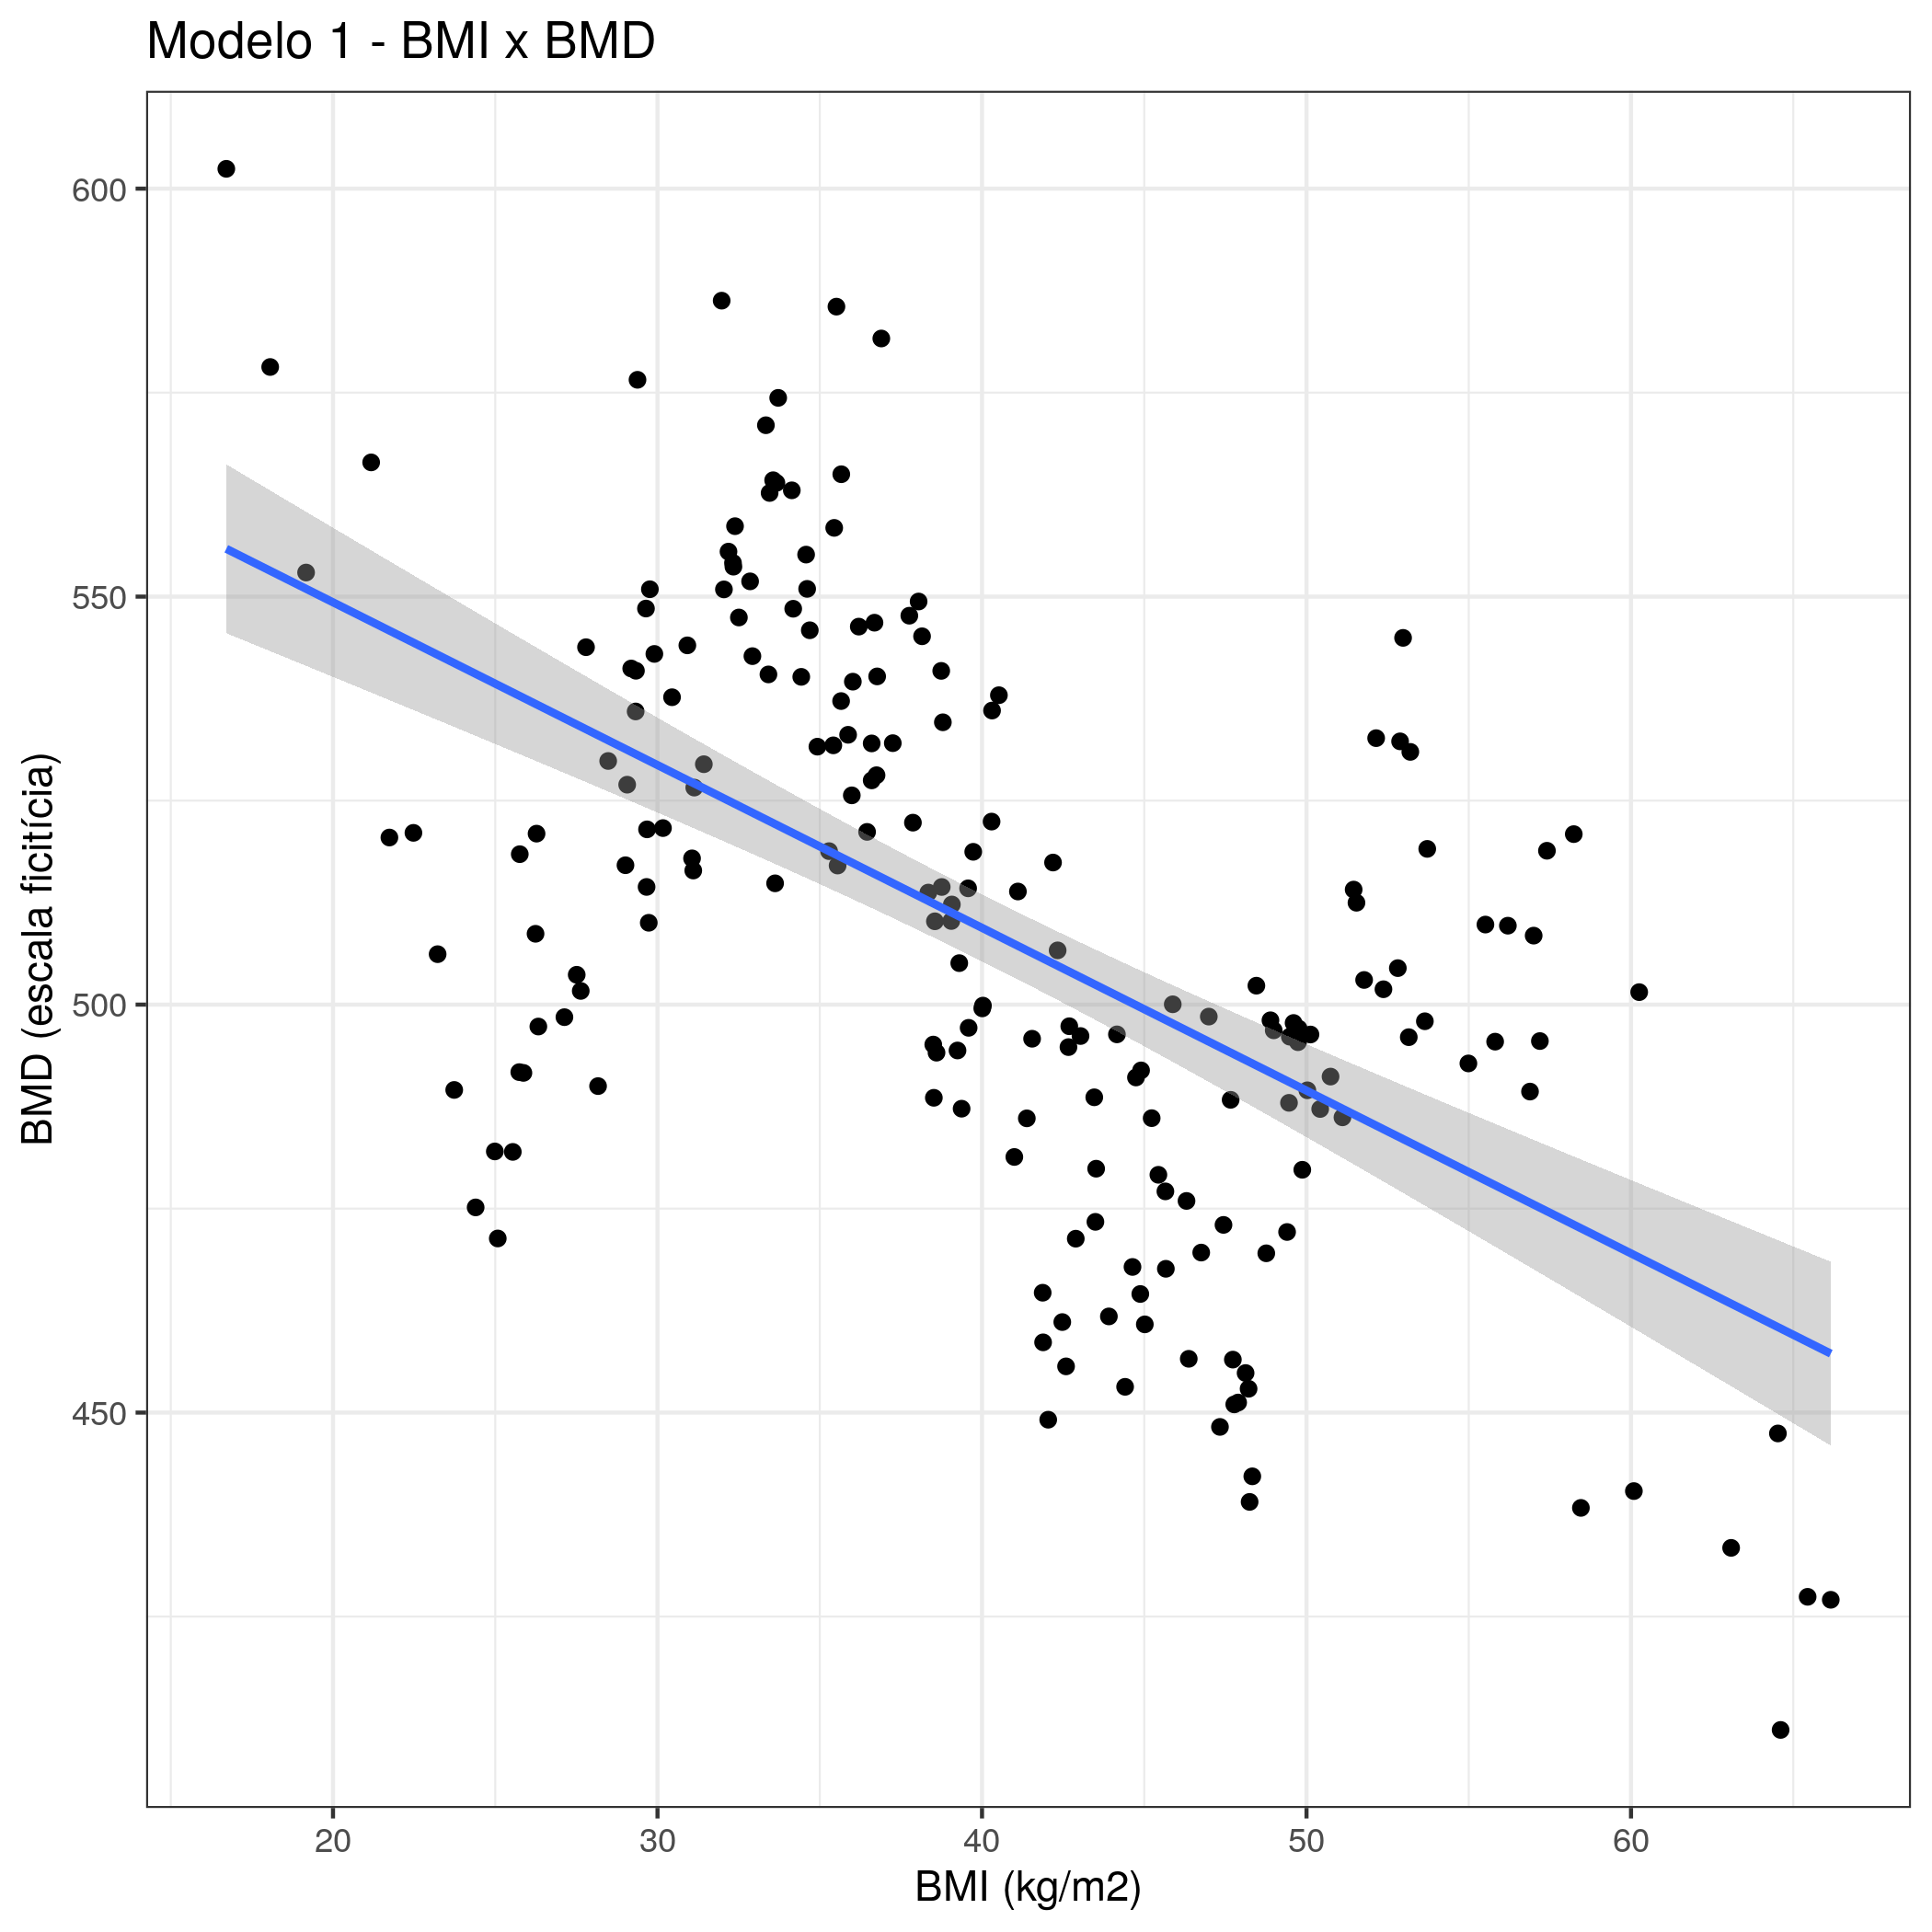
\includegraphics[height=.6\textheight]{Cap31-32/pratica-rlm1}
    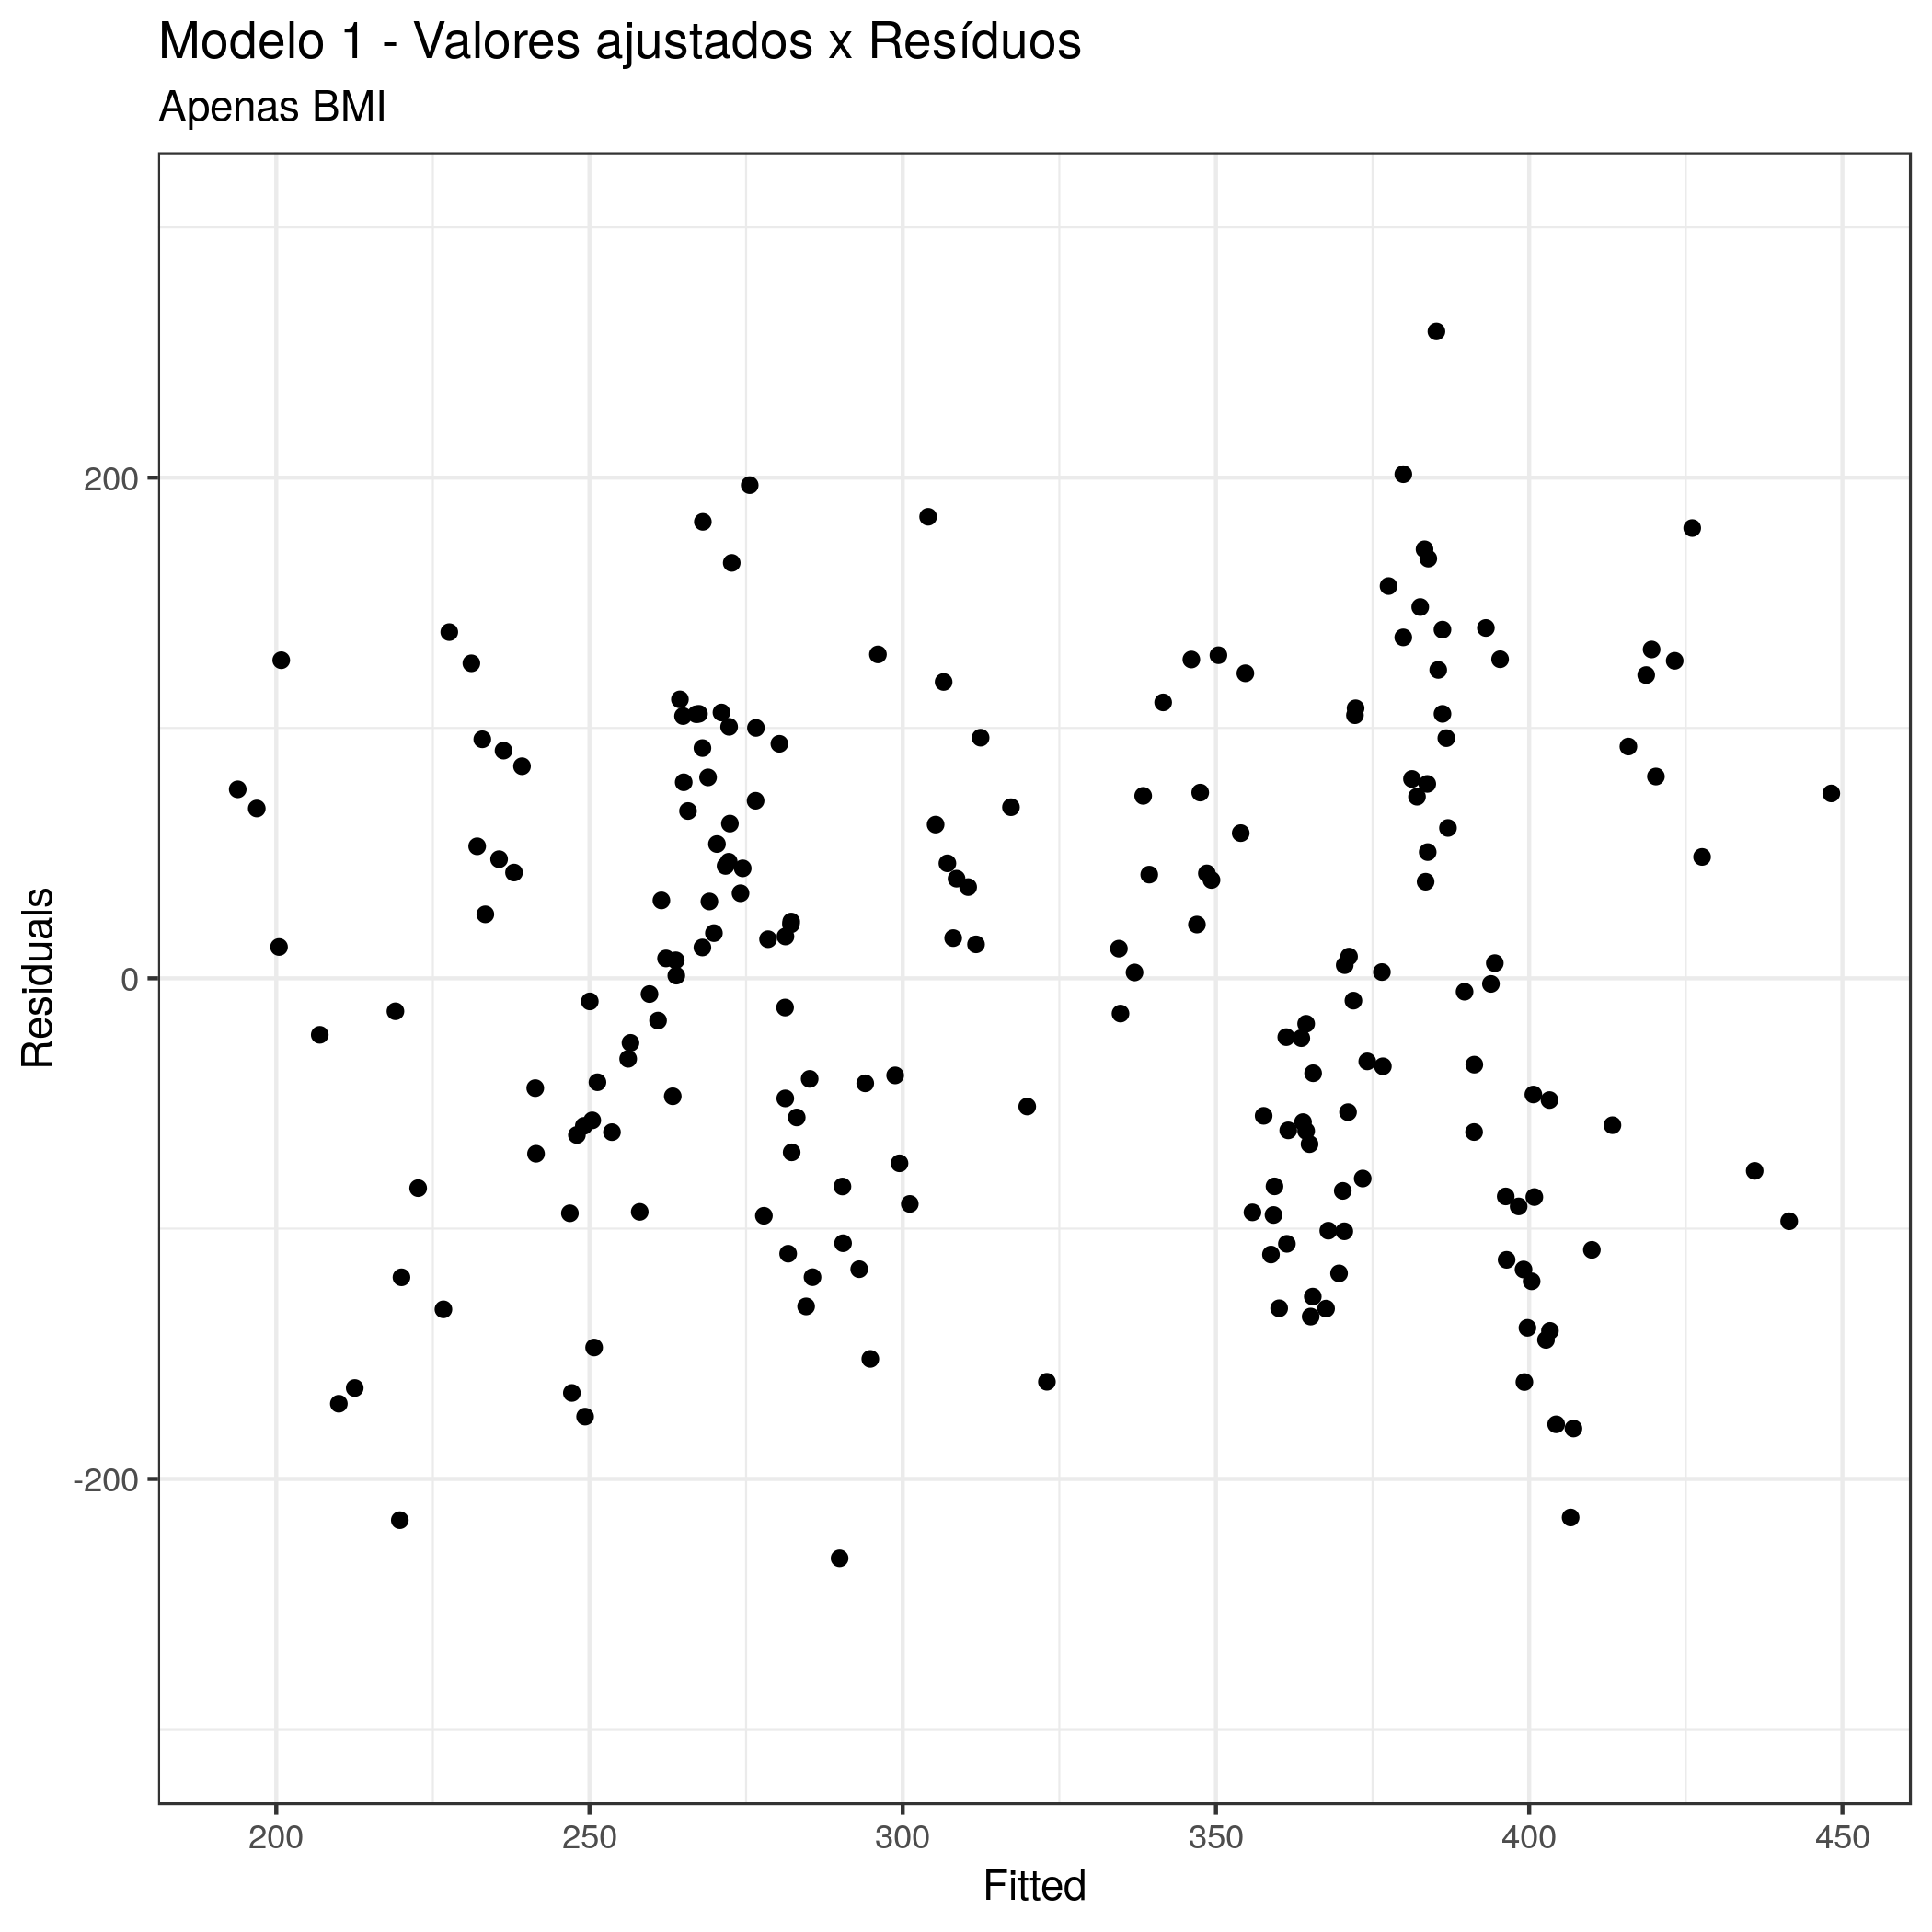
\includegraphics[height=.6\textheight]{Cap31-32/pratica-rlm1-resid}
\end{center}
\end{frame}

\begin{frame}{\scriptsize }
  \begin{exampleblock}{Modelo 1 completo}
    \footnotesize
    \begin{displaymath}
      \text{BMD} =607.37 -1.98 \times\text{BMI}
    \end{displaymath}
  \end{exampleblock}

  \bigskip
  \begin{exampleblock}{Interpretação}
    \footnotesize
    As participantes perdem, na média, 1.98 unidades de BMD para cada incremento unitário do BMI.

    \bigskip
    Este é o chamado resultado bruto. Agora vamos ajustá-lo com outros preditores.
  \end{exampleblock}
\end{frame}

\begin{frame}{\scriptsize }
  \begin{center}
    Agora vamos ver se a etnia tem algum efeito
  \end{center}
\end{frame}

\begin{frame}{\scriptsize Modelo 2}
  \begin{center}
    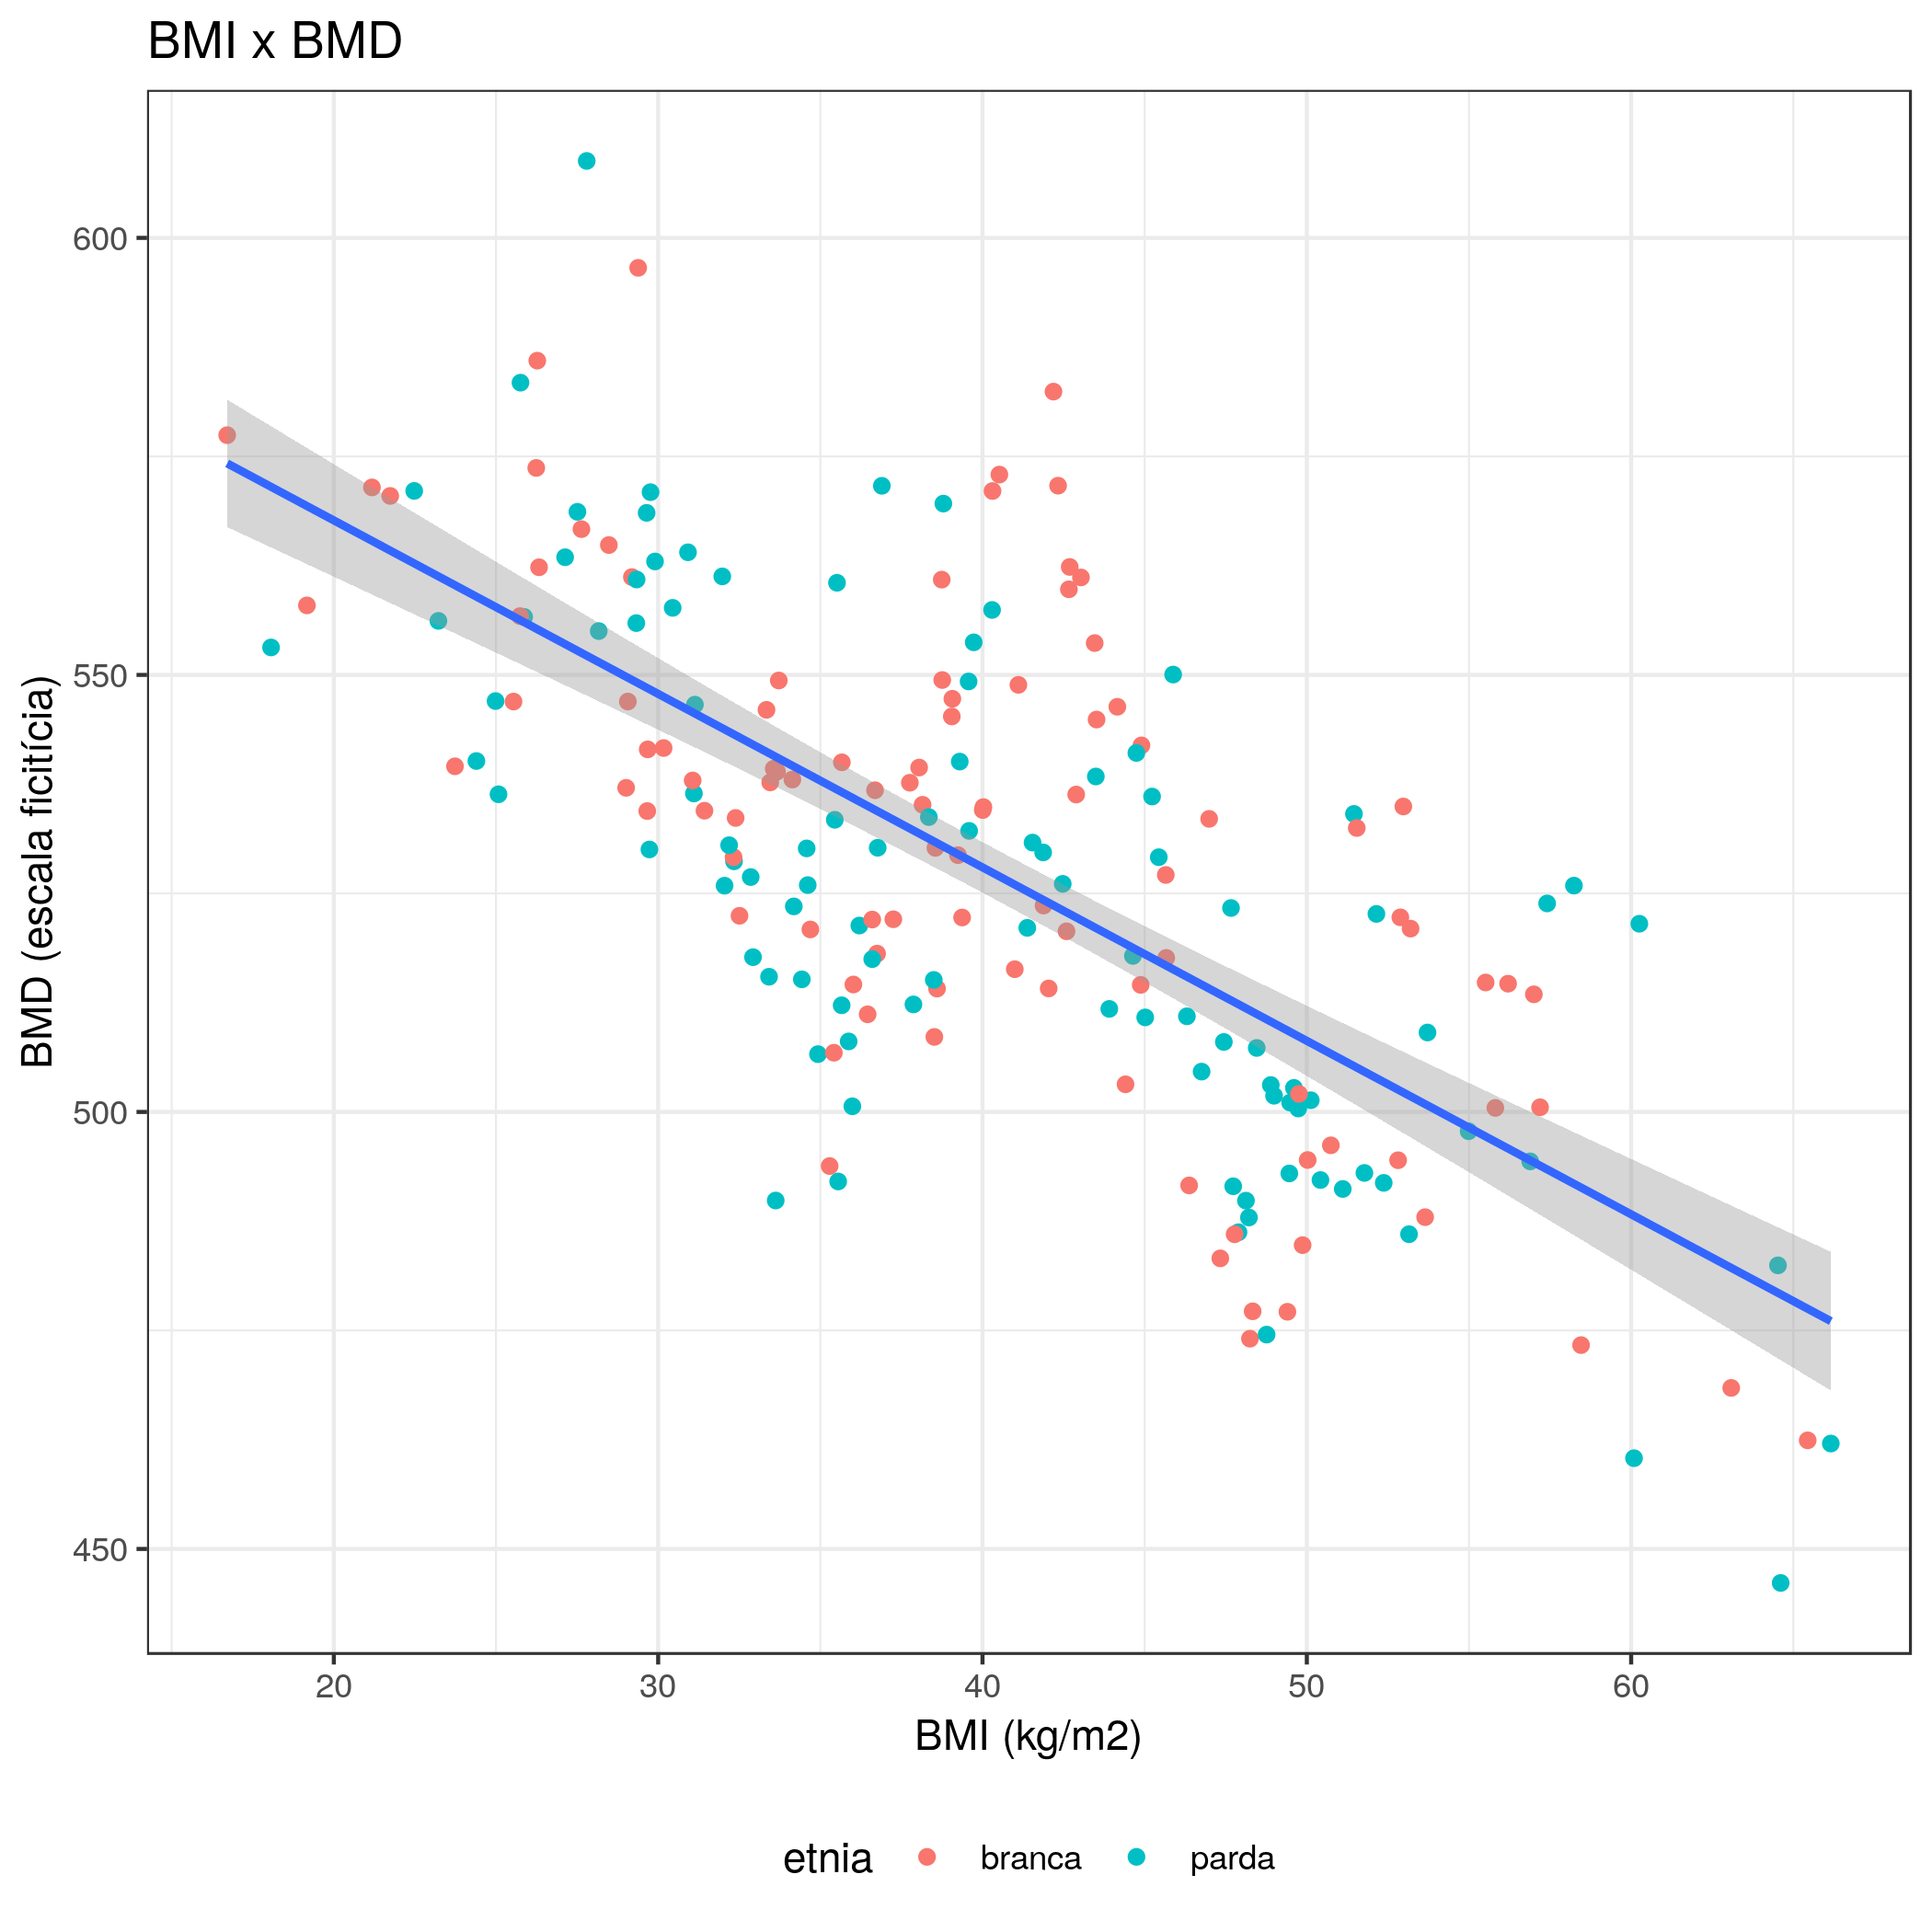
\includegraphics[height=.9\textheight]{Cap31-32/pratica-rlm2_0}
  \end{center}
\end{frame}

\begin{frame}{\scriptsize Quais são as variáveis?}
  \begin{itemize}
    \footnotesize
  \item Dependente: BMD (contínua)
  \item Independente: BMI (contínua)
  \item Independente: etnia (categórica -- binária)
  \end{itemize}
  \vfill
  \begin{block}{Esta relação pode ser expressa como}
    \footnotesize
    \begin{displaymath}
      \text{BMD} \sim \text{BMI} + \text{etnia}
    \end{displaymath}
  \end{block}
\end{frame}

\begin{frame}{\scriptsize Componentes do modelo 2}
  \begin{block}{\footnotesize Versão simplificada (apenas variáveis)}
    \footnotesize
    \begin{displaymath}
      \text{BMD} \sim \text{BMI} + \text{etnia}
    \end{displaymath}
  \end{block}
  \bigskip
  \bigskip
  \begin{block}{Modelo completo}
    \begin{displaymath}
      \text{BMD} =\beta_0 + \beta_1 \text{(BMI)} + \beta_2 \text{(etnia)} +\varepsilon
    \end{displaymath}
  \end{block}
  \vfill
  % \footnotesize
  % Hipótese: $\varepsilon$ é um erro aleatório \footnote{\scriptsize residual -- não é explicado pela relação entre as variáveis do modelo} normalmente distribuído e centrado em zero -- a incerteza que não pode ser controlada.
\end{frame}

\begin{frame}[fragile]{\scriptsize }
  \begin{center}
    \begin{exampleblock}{Modelo 2}
      \tiny
\begin{verbatim}
Residuals:
    Min      1Q  Median      3Q     Max 
-48.543 -14.299  -2.799  14.044  58.875 

Coefficients:
            Estimate Std. Error t value Pr(>|t|)    
(Intercept)  609.236      6.097  99.917   <2e-16 ***
BMI           -1.977      0.144 -13.729   <2e-16 ***
etniaparda    -4.351      2.922  -1.489    0.138    
---
Signif. codes:  0 ‘***’ 0.001 ‘**’ 0.01 ‘*’ 0.05 ‘.’ 0.1 ‘ ’ 1

Residual standard error: 20.65 on 197 degrees of freedom
Multiple R-squared:  0.4941,	Adjusted R-squared:  0.489 
F-statistic: 96.21 on 2 and 197 DF,  p-value: < 2.2e-16
\end{verbatim}
    \end{exampleblock}
  \end{center}
\end{frame}

\begin{frame}{\scriptsize Modelo 2}
  \begin{center}
    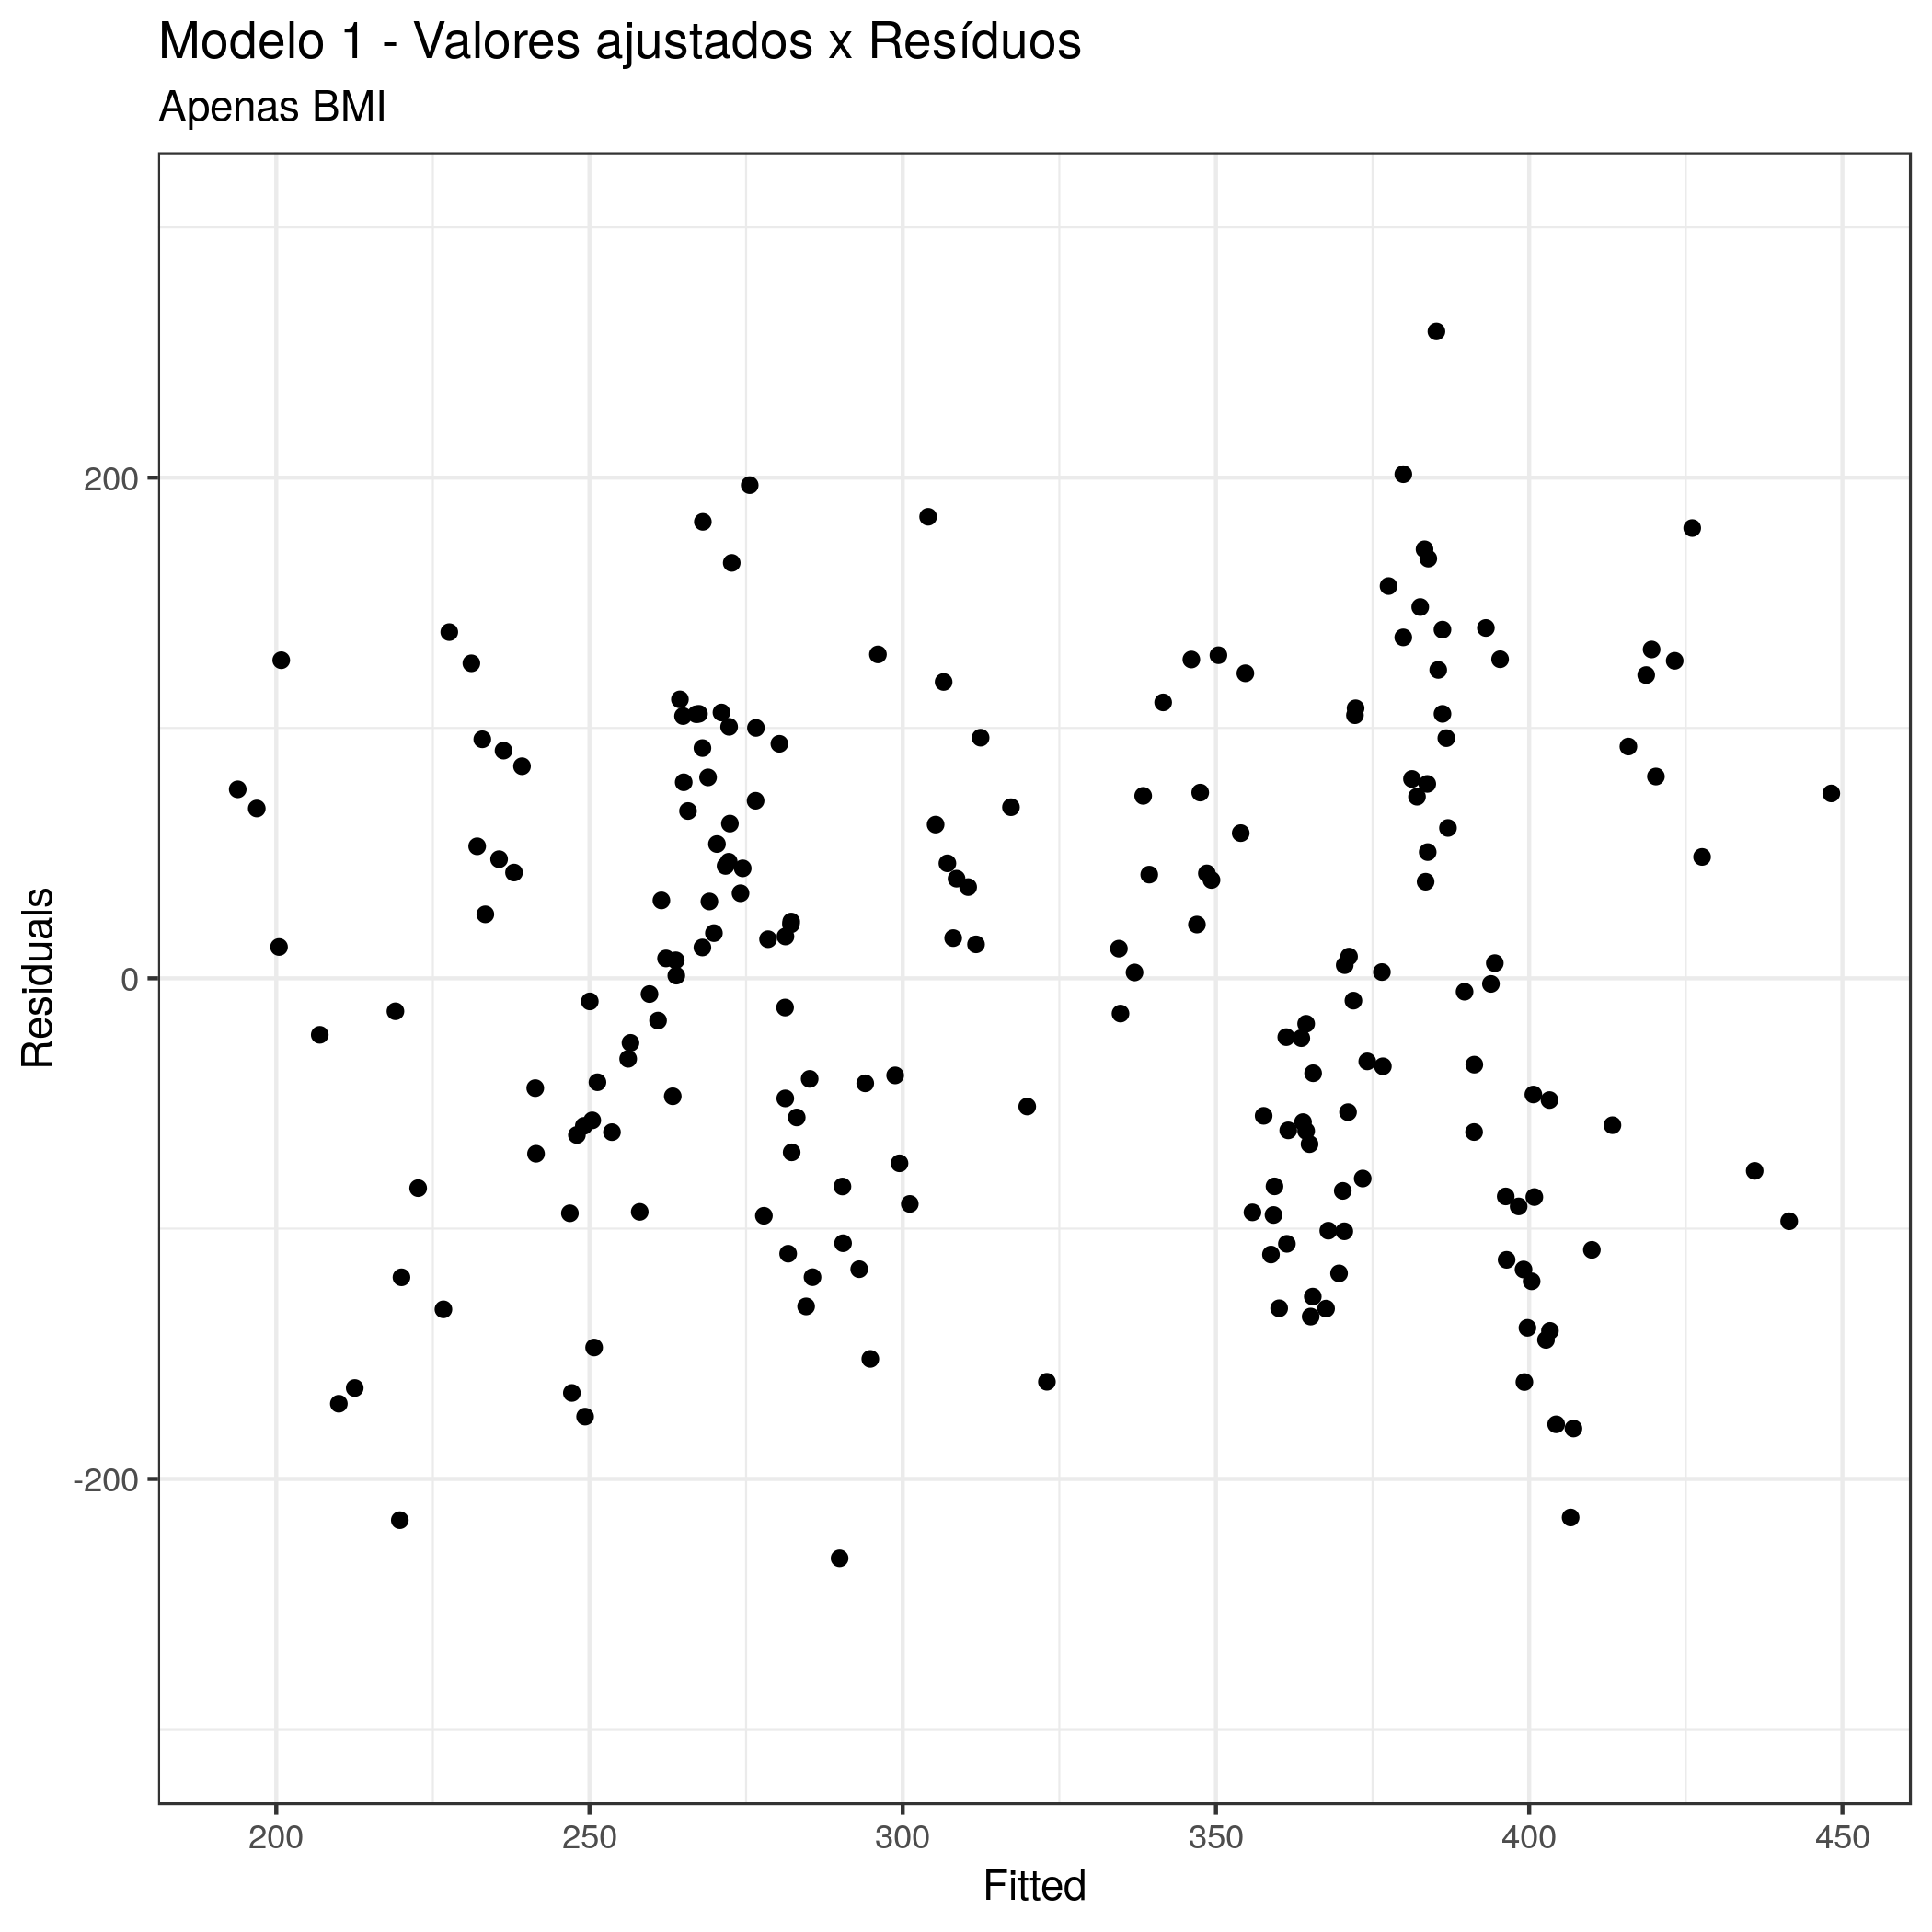
\includegraphics[height=.6\textheight]{Cap31-32/pratica-rlm1-resid}
    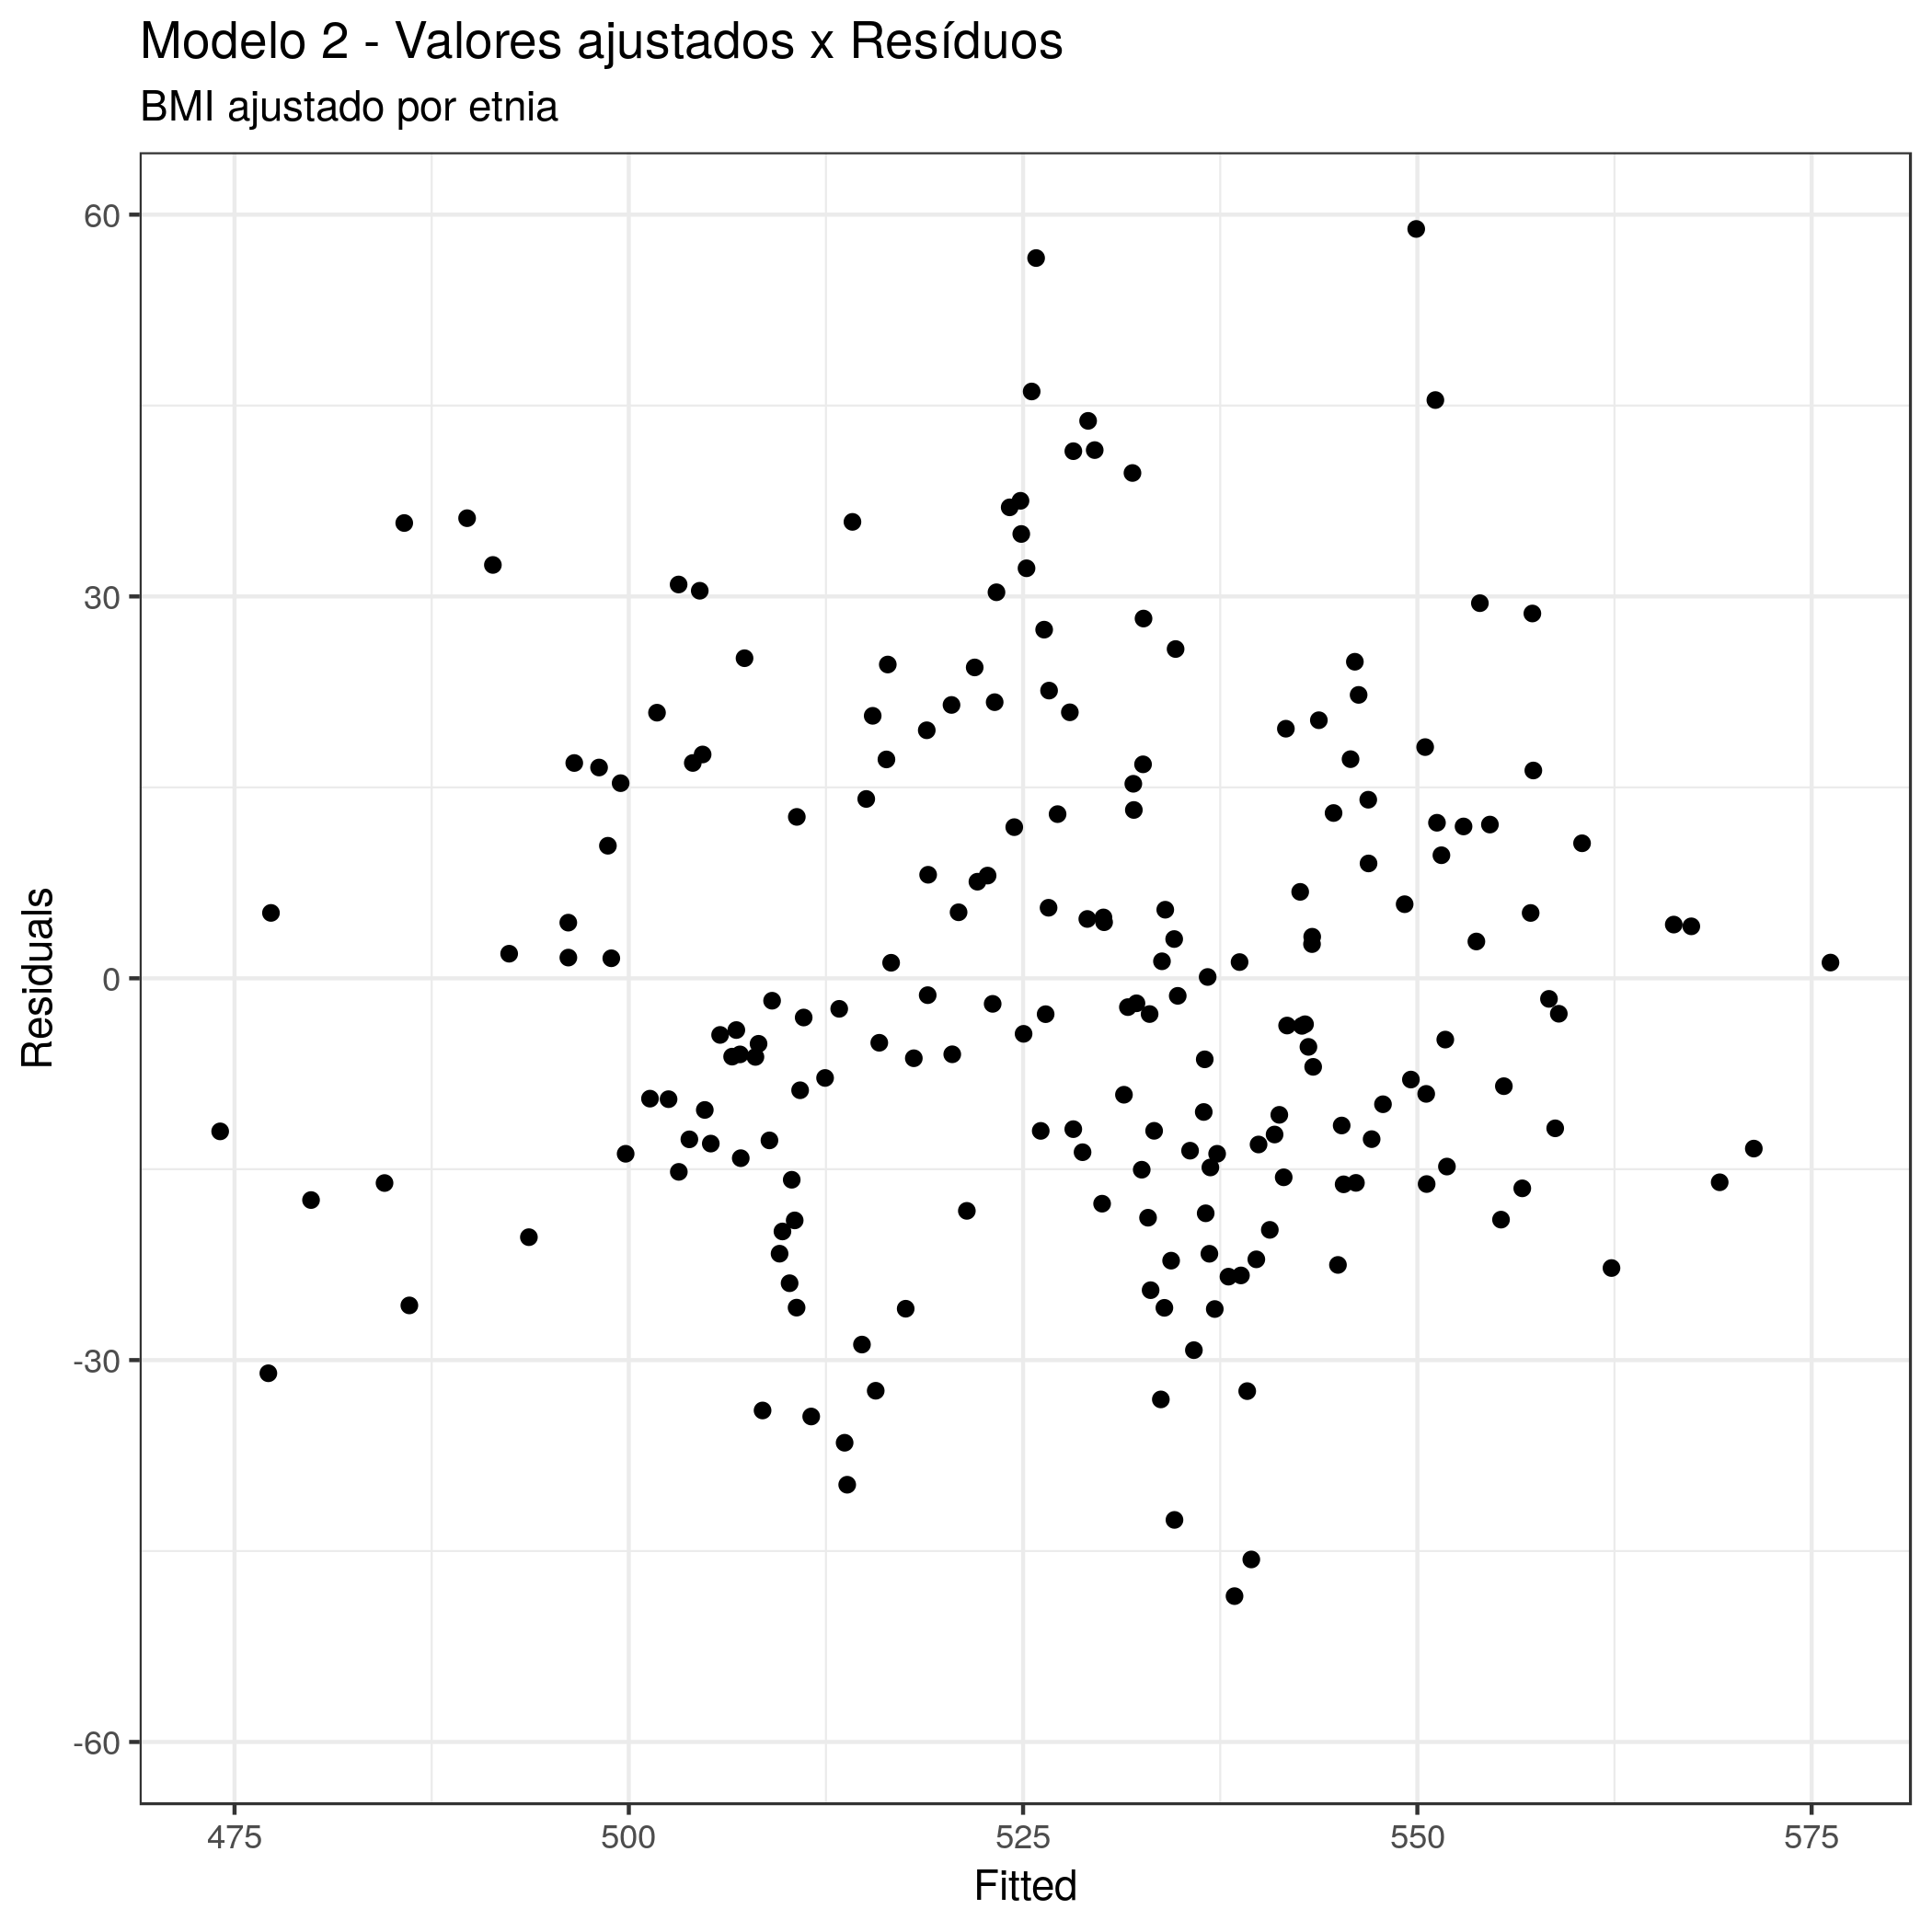
\includegraphics[height=.6\textheight]{Cap31-32/pratica-rlm2_0-resid}
  \end{center}
\end{frame}

\begin{frame}{\scriptsize }
  \begin{center}
    Que outra variável os pesquisadores deveriam ter investigado?
  \end{center}
\end{frame}

\begin{frame}{\scriptsize Modelo 2.1 -- idade}
  \begin{center}
    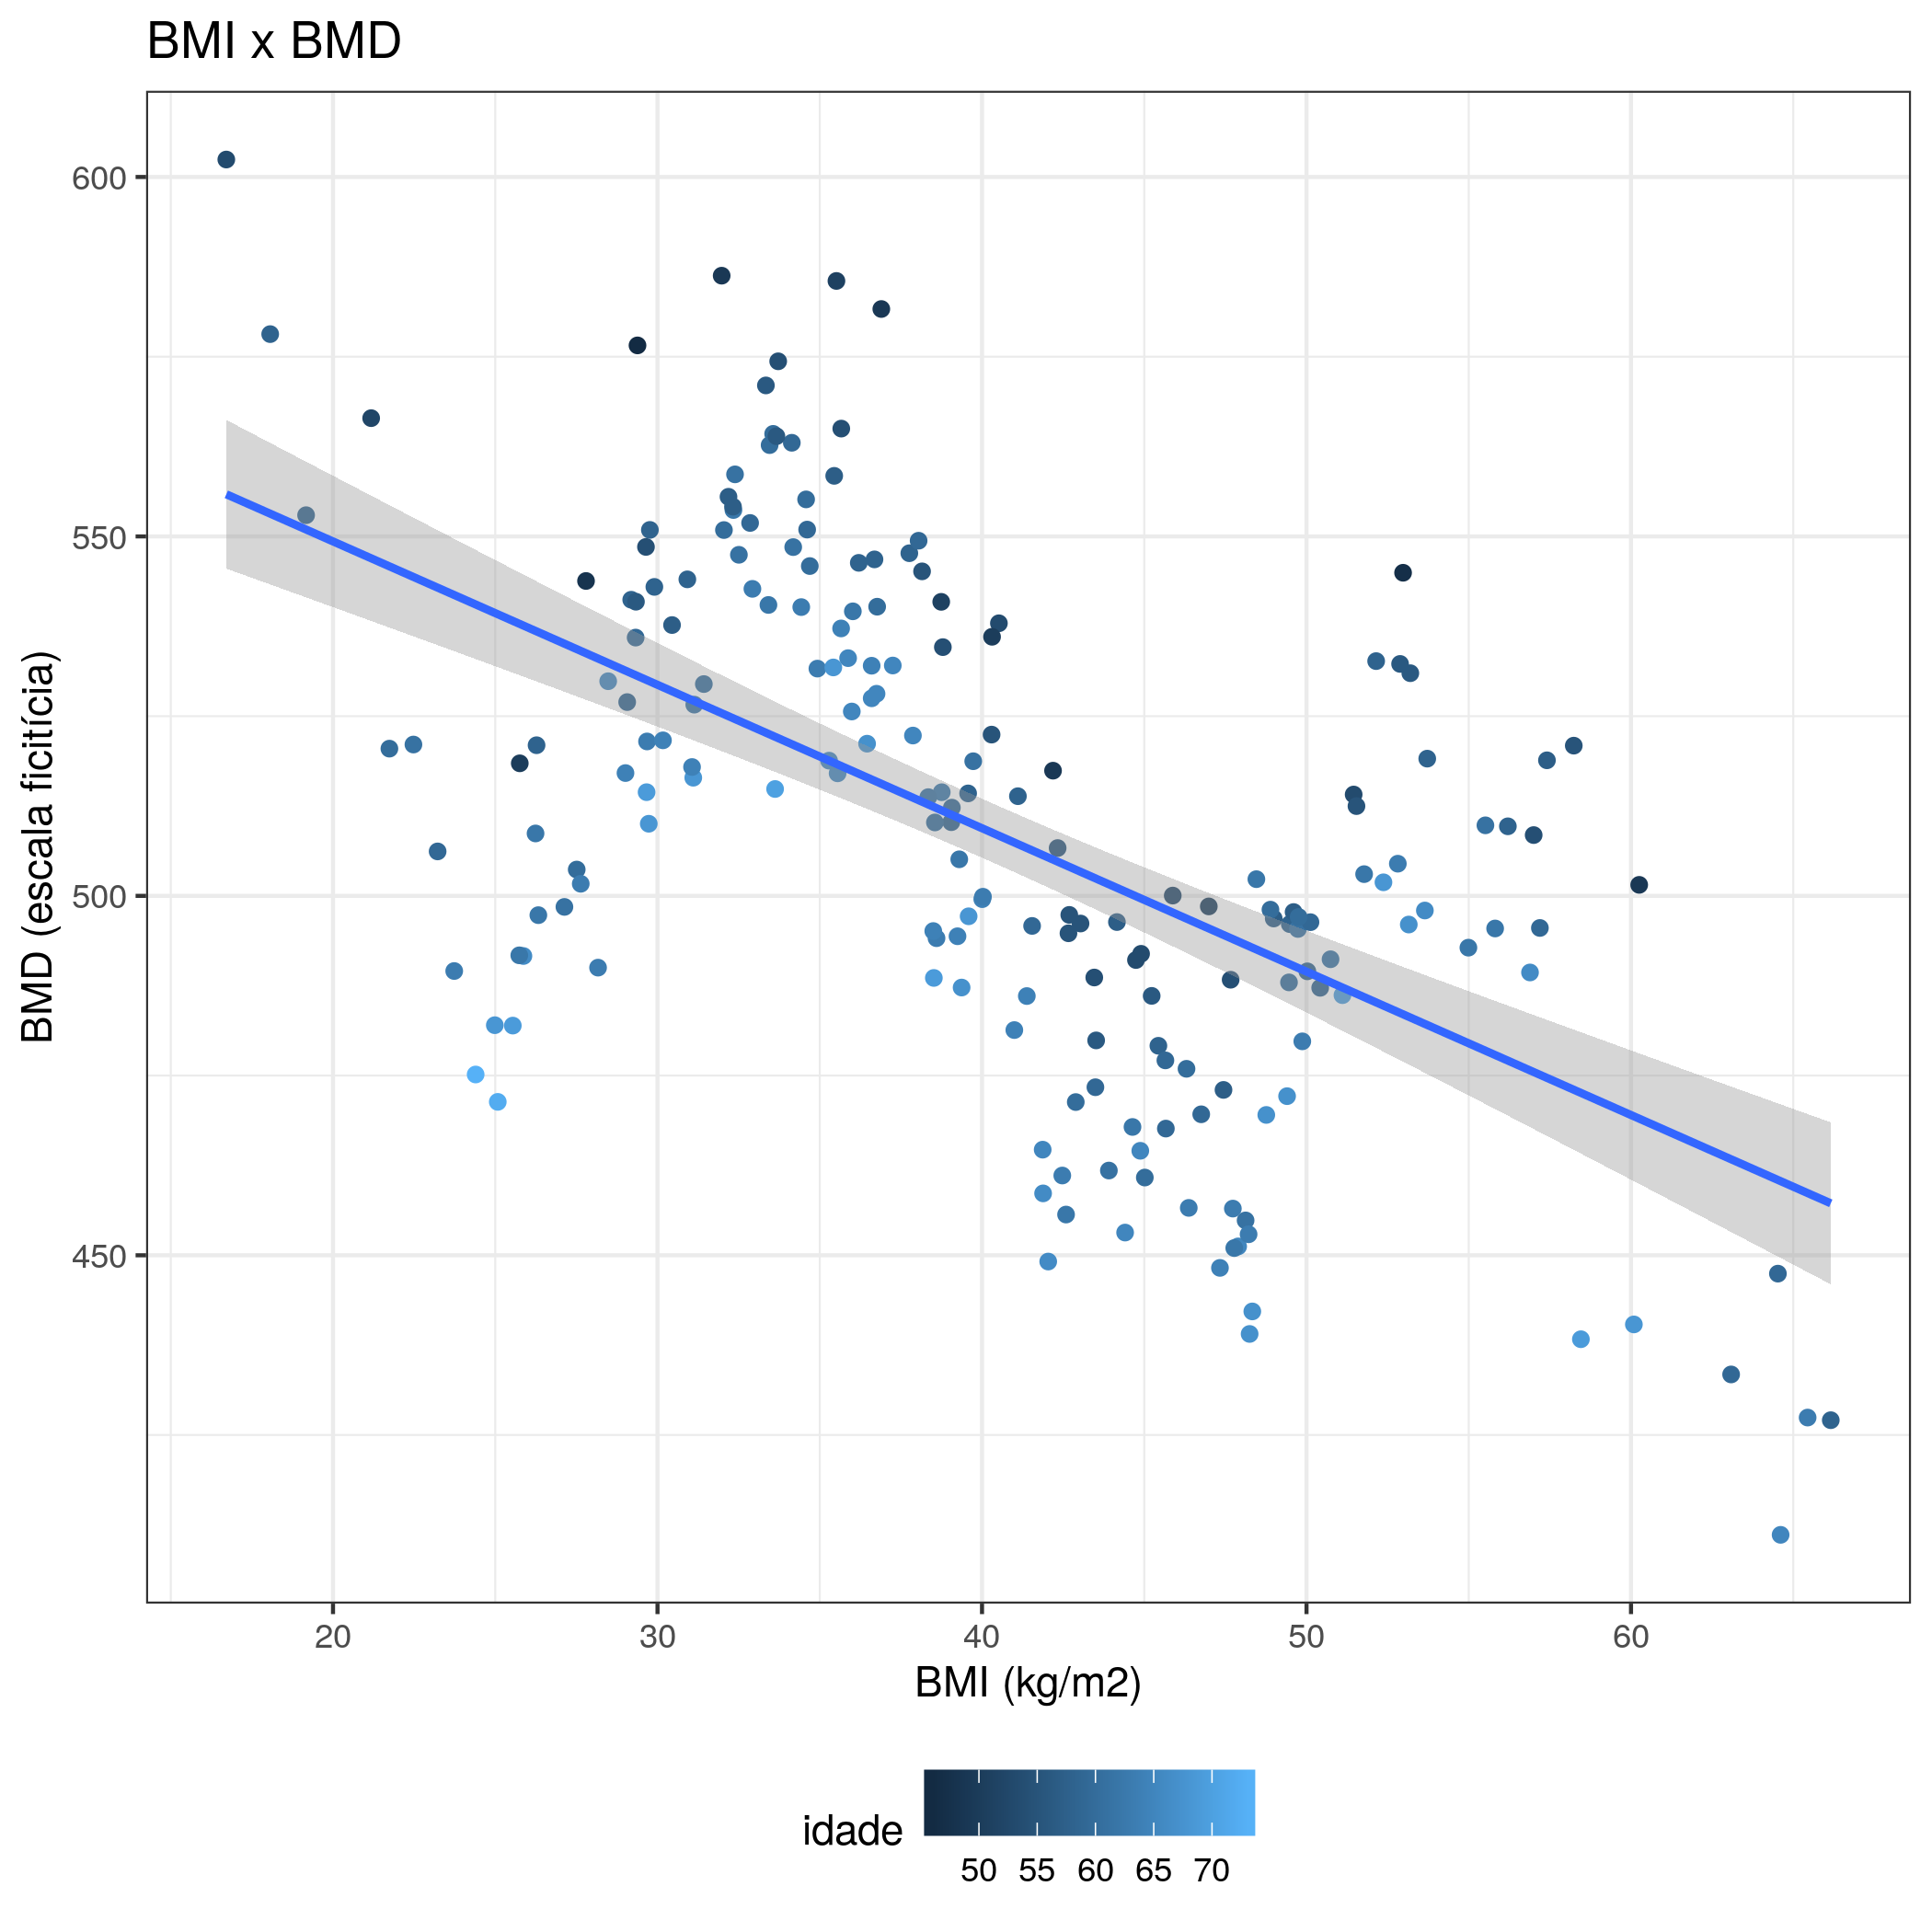
\includegraphics[height=.9\textheight]{Cap31-32/pratica-rlm2_1}
  \end{center}
\end{frame}

\begin{frame}{\scriptsize Quais são as variáveis?}
  \begin{itemize}
    \footnotesize
  \item Dependente: BMD (contínua)
  \item Independente: BMI (contínua)
  \item Independente: idade (contínua)
  \end{itemize}
  \vfill
  \begin{block}{Esta relação pode ser expressa como}
    \footnotesize
    \begin{displaymath}
      \text{BMD} \sim \text{BMI} + \text{idade}
    \end{displaymath}
  \end{block}
\end{frame}

\begin{frame}{\scriptsize Componentes do modelo 2.1}
  \begin{block}{\footnotesize Versão simplificada (apenas variáveis)}
    \footnotesize
    \begin{displaymath}
      \text{BMD} \sim \text{BMI} + \text{idade}
    \end{displaymath}
  \end{block}
  \bigskip
  \bigskip
  \begin{block}{Modelo completo}
    \footnotesize
    \begin{displaymath}
      \text{BMD} =\beta_0 + \beta_1 \text{(BMI)} + \beta_2 \text{(idade)} +\varepsilon
    \end{displaymath}
  \end{block}
  \vfill
  % \footnotesize
  % Hipótese: $\varepsilon$ é um erro aleatório \footnote{\scriptsize residual -- não é explicado pela relação entre as variáveis do modelo} normalmente distribuído e centrado em zero -- a incerteza que não pode ser controlada.
\end{frame}

\begin{frame}[fragile]{\scriptsize }
  \begin{center}
    \begin{exampleblock}{Modelo 2.1}
      \tiny
\begin{verbatim}
Residuals:
    Min      1Q  Median      3Q     Max 
-30.484 -12.318   0.865  11.618  32.679 

Coefficients:
             Estimate Std. Error t value Pr(>|t|)    
(Intercept) 790.51012   12.57103   62.88   <2e-16 ***
BMI          -2.02336    0.09757  -20.74   <2e-16 ***
idade        -3.01619    0.19603  -15.39   <2e-16 ***
---
Signif. codes:  0 ‘***’ 0.001 ‘**’ 0.01 ‘*’ 0.05 ‘.’ 0.1 ‘ ’ 1

Residual standard error: 14 on 197 degrees of freedom
Multiple R-squared:  0.7676,	Adjusted R-squared:  0.7653 
F-statistic: 325.4 on 2 and 197 DF,  p-value: < 2.2e-16
\end{verbatim}
    \end{exampleblock}
  \begin{exampleblock}{Modelo 2.1 completo}
    \footnotesize
    \begin{displaymath}
      \text{BMD} =790.51 + -2.02 \times\text{BMI} -3.02 \times\text{idade}
    \end{displaymath}
  \end{exampleblock}
  \end{center}
\end{frame}

\begin{frame}{\scriptsize Modelo 2.1}
  \begin{center}
    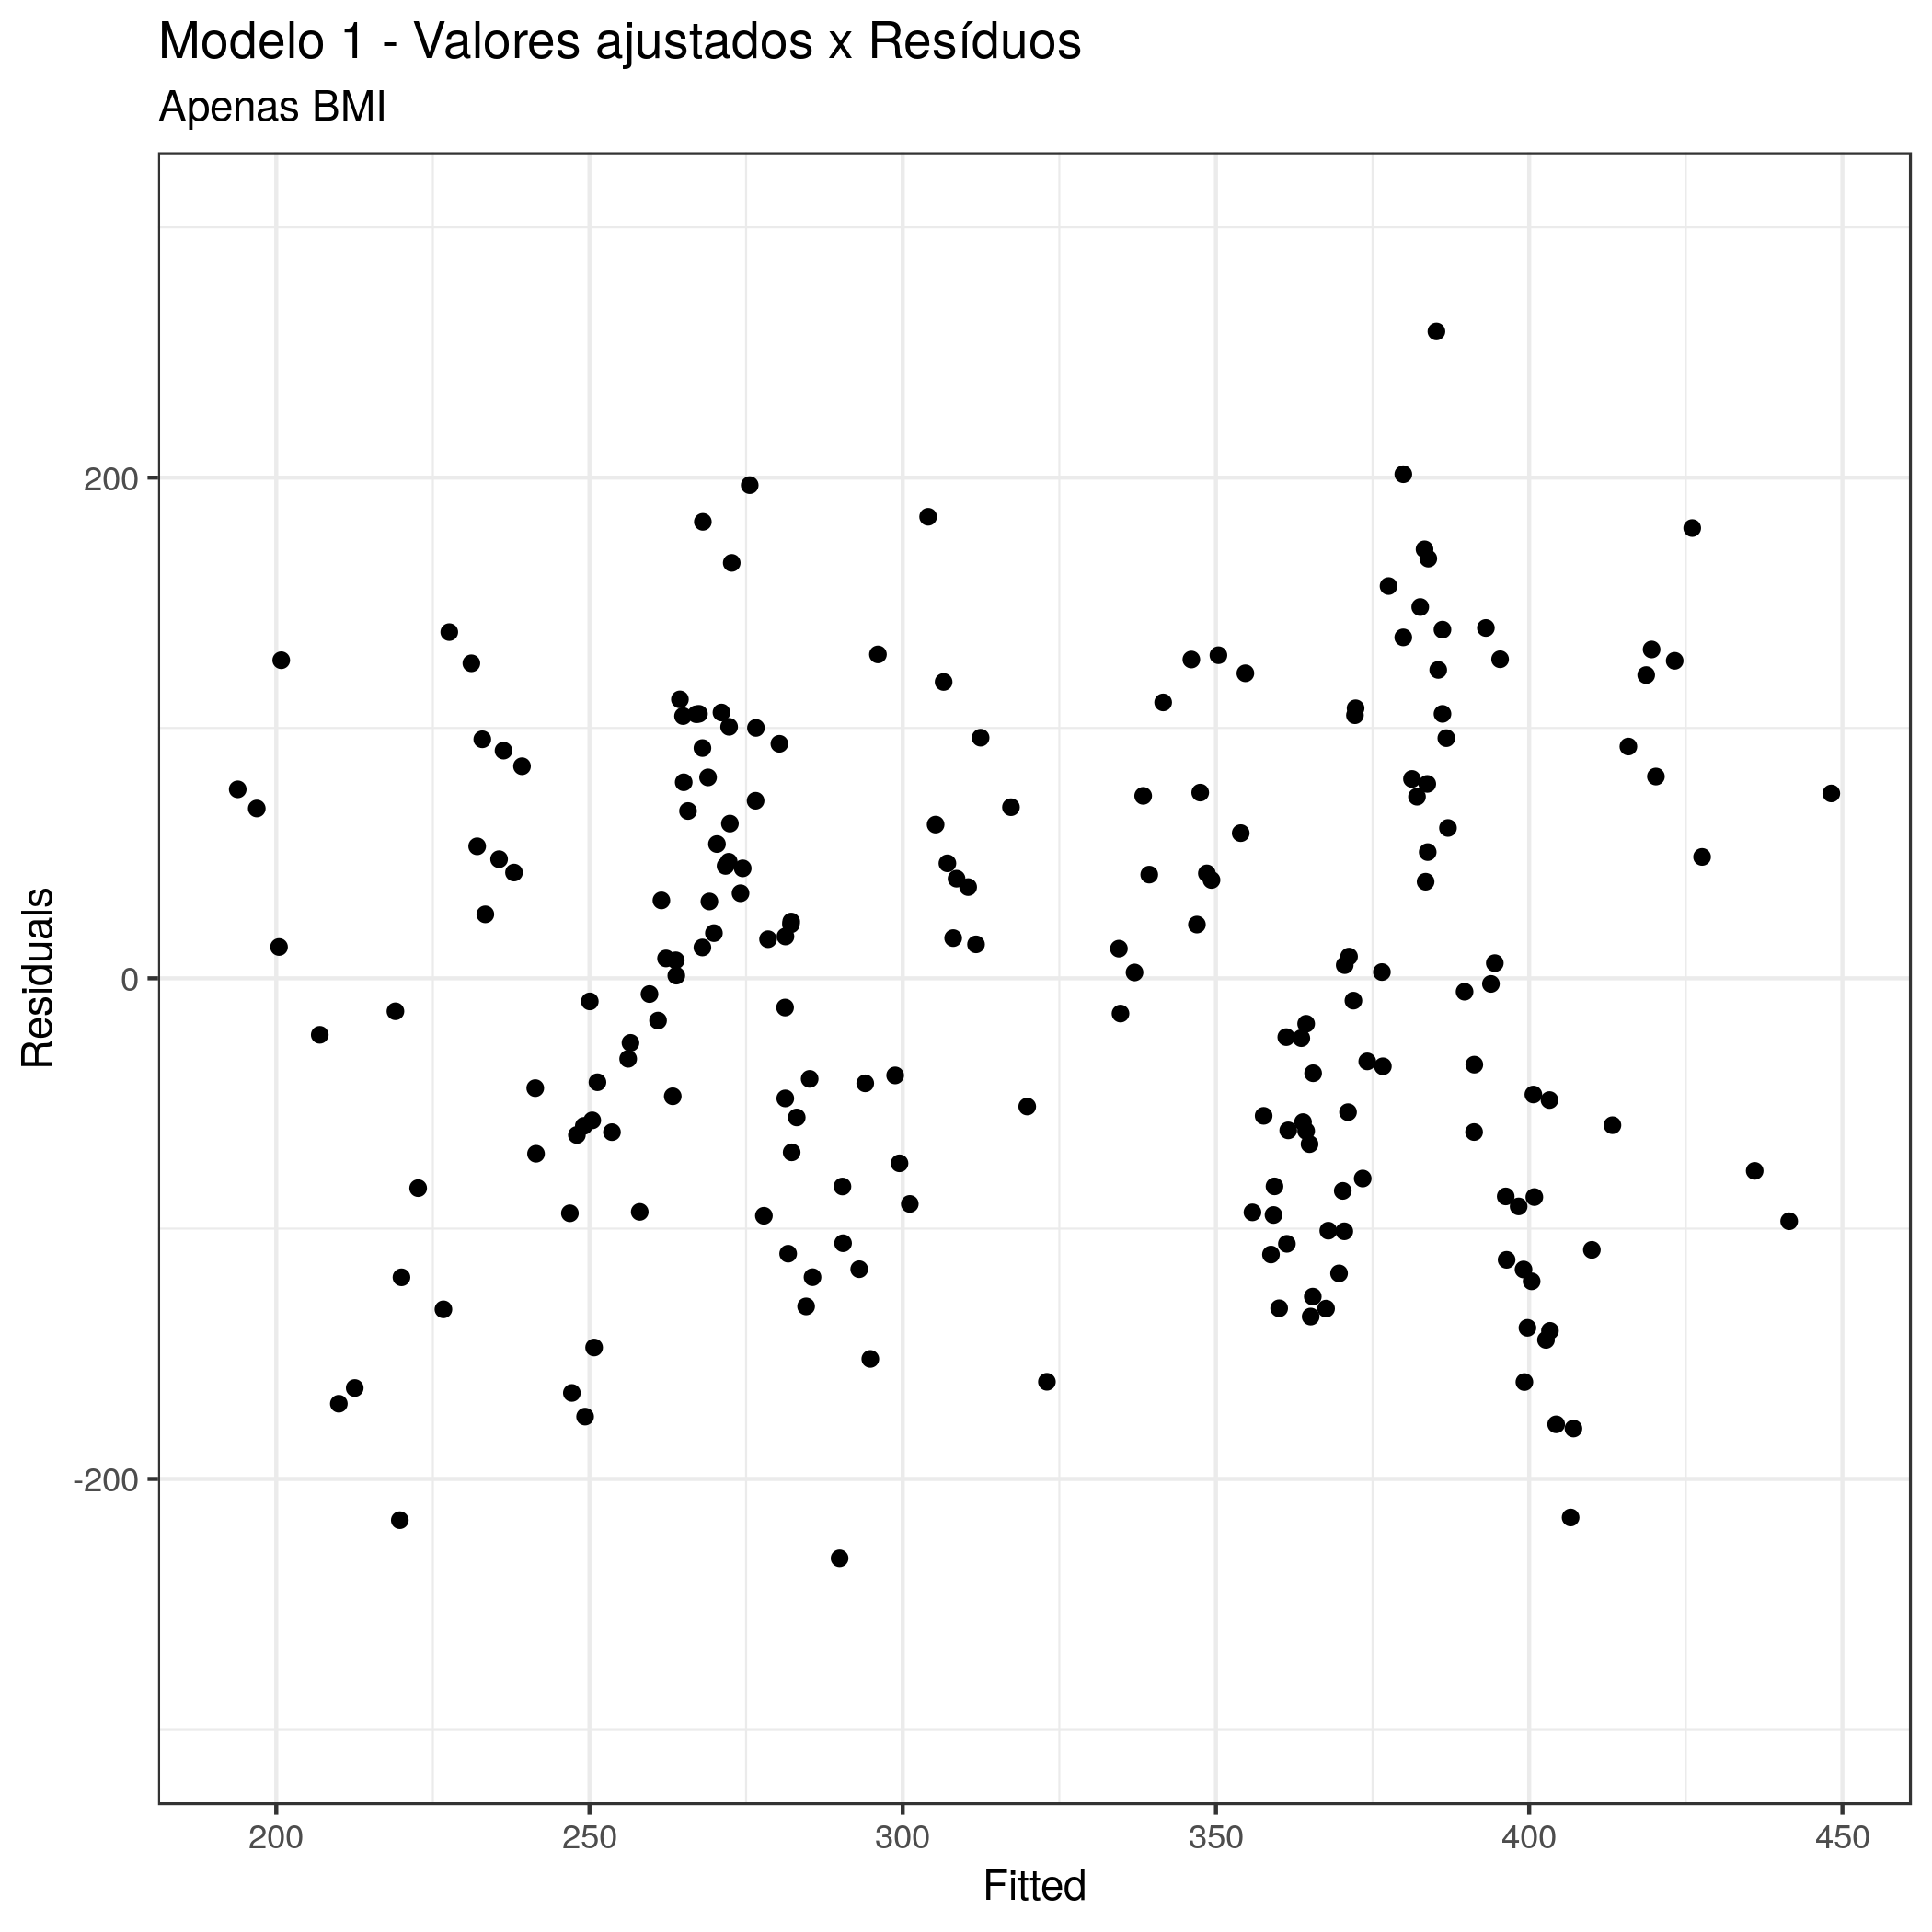
\includegraphics[height=.6\textheight]{Cap31-32/pratica-rlm1-resid}
    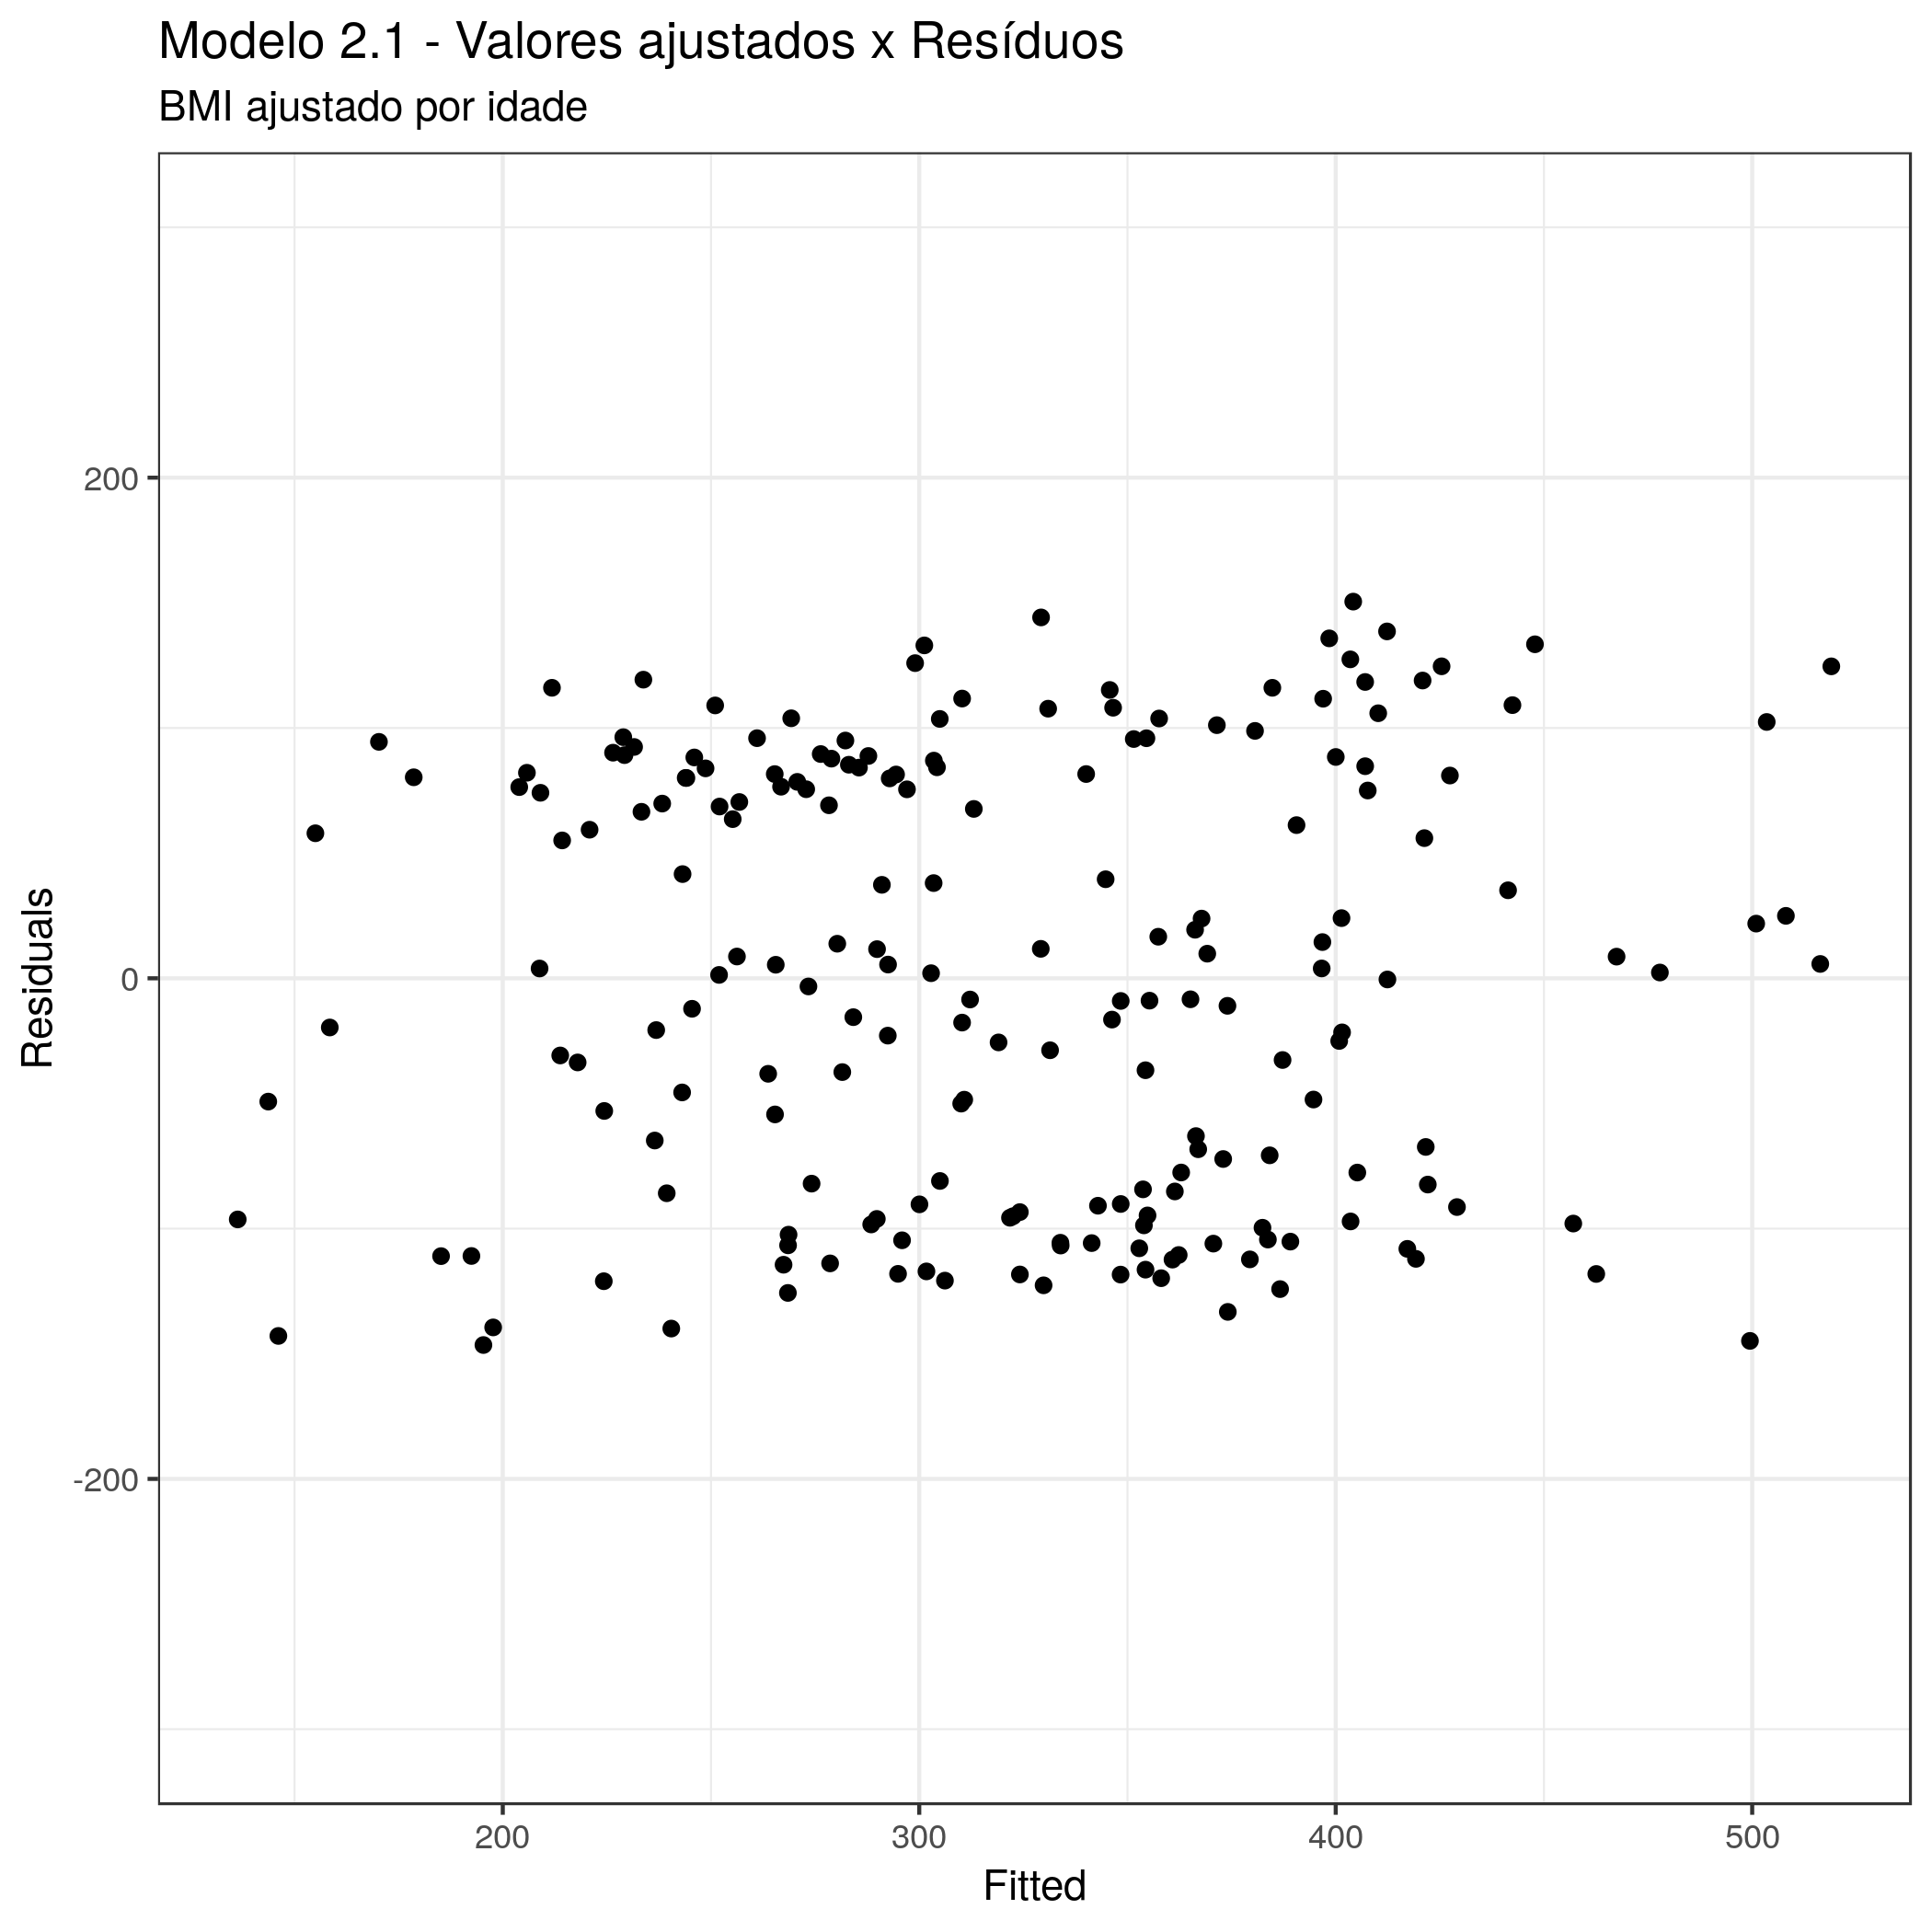
\includegraphics[height=.6\textheight]{Cap31-32/pratica-rlm2_1-resid}
  \end{center}
\end{frame}

\begin{frame}{\scriptsize }
  \begin{exampleblock}{Modelo 2.1 completo}
    \footnotesize
    \begin{displaymath}
      \text{BMD} =790.51 + -2.02 \times\text{BMI} -3.02 \times\text{idade}
    \end{displaymath}
  \end{exampleblock}
  \begin{block}{}
    \footnotesize
    As participantes perdem, na média, 1.98 unidades de BMD para cada incremento unitário do BMI (resultado bruto).

    \bigskip
    Após ajustar pela idade, o resultado é 2.02.
  \end{block}
\end{frame}

\begin{frame}{\scriptsize }
  \begin{center}
    Que outra variável os pesquisadores deveriam ter investigado?
  \end{center}
\end{frame}

\begin{frame}{\scriptsize Modelo 2.2 -- quantidade de hormônio}
  \begin{center}
    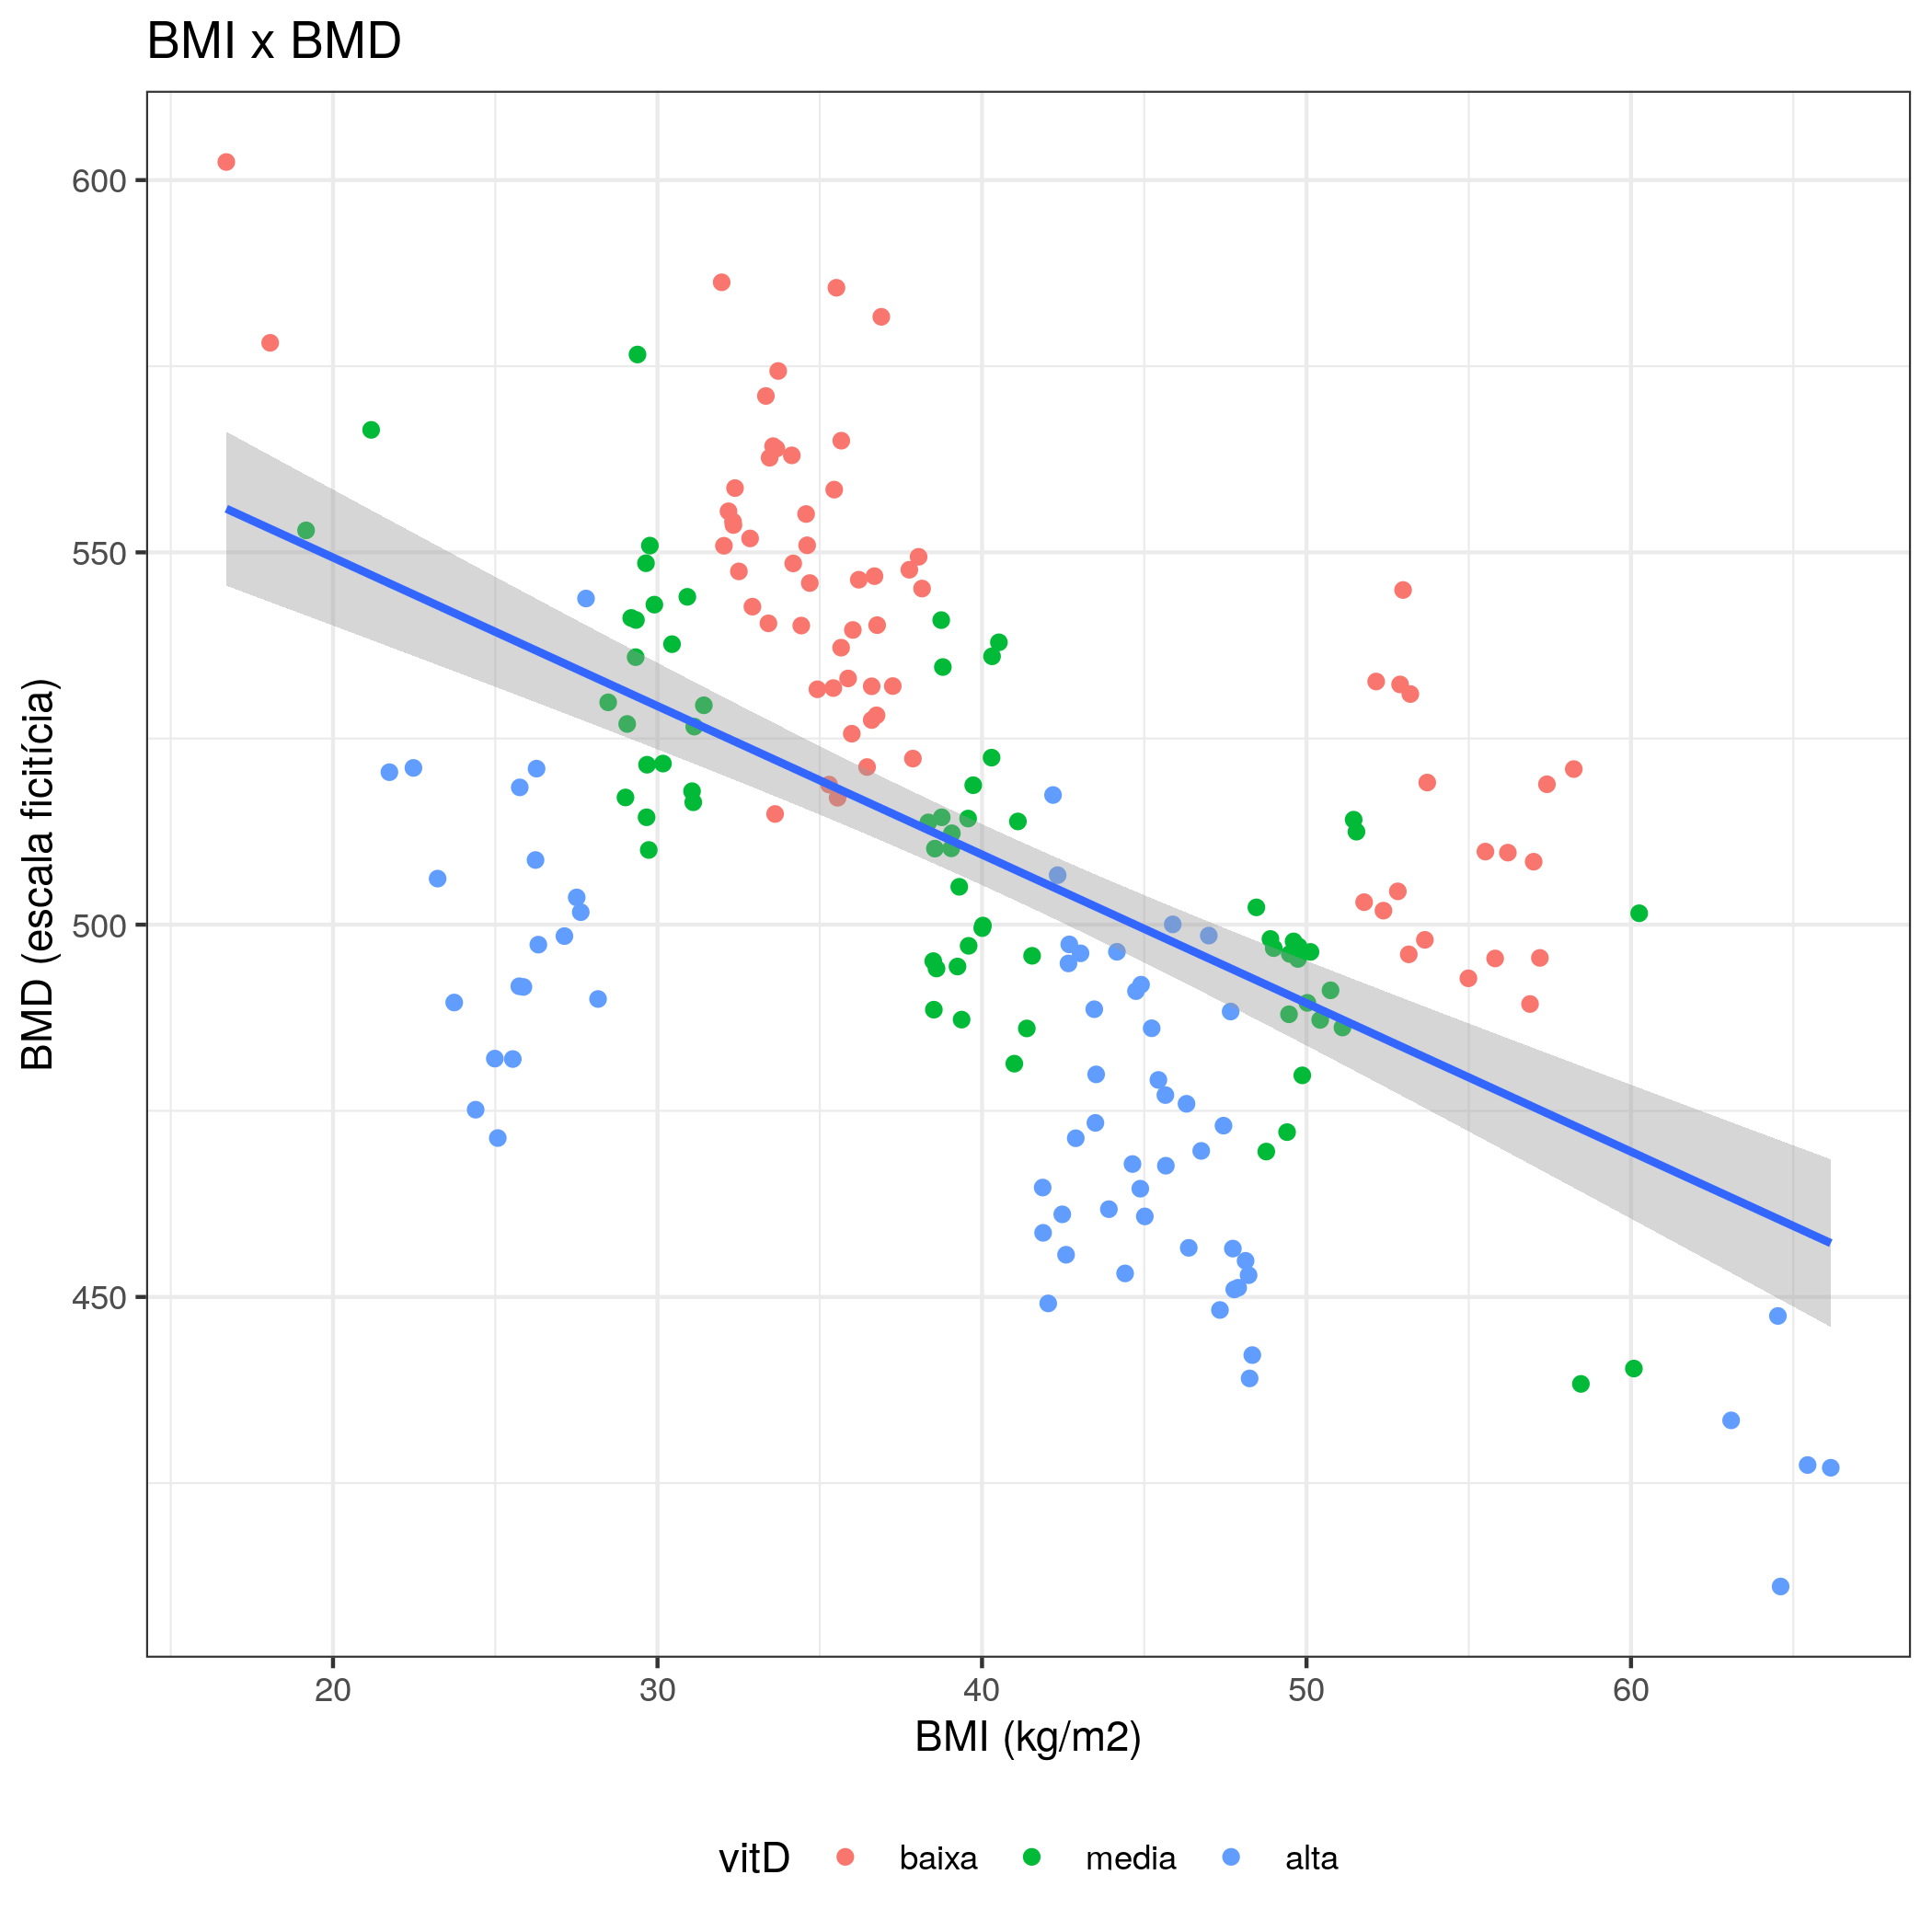
\includegraphics[height=.9\textheight]{Cap31-32/pratica-rlm2_2}
  \end{center}
\end{frame}

\begin{frame}{\scriptsize Quais são as variáveis?}
  \begin{itemize}
    \footnotesize
  \item Dependente: BMD (contínua)
  \item Independente: BMI (contínua)
  \item Independente: hormônio (categórica -- 3 níveis)
  \end{itemize}
  \vfill
  \begin{block}{Esta relação pode ser expressa como}
    \footnotesize
    \begin{displaymath}
      \text{BMD} \sim \text{BMI} + \text{hormônio}
    \end{displaymath}
  \end{block}
\end{frame}

\begin{frame}{\scriptsize Componentes do modelo 2.2}
  \begin{block}{\footnotesize Versão simplificada (apenas variáveis)}
    \footnotesize
    \begin{displaymath}
      \text{BMD} \sim \text{BMI} + \text{hormônio}
    \end{displaymath}
  \end{block}
  \bigskip
  \bigskip
  \begin{block}{Modelo completo}
    \footnotesize
    \begin{displaymath}
      \text{BMD} =\beta_0 + \beta_1 \text{(BMI)} + \beta_2 \text{(hormônio)} +\varepsilon
    \end{displaymath}
  \end{block}
  \vfill
  % \footnotesize
  % Hipótese: $\varepsilon$ é um erro aleatório \footnote{\scriptsize residual -- não é explicado pela relação entre as variáveis do modelo} normalmente distribuído e centrado em zero -- a incerteza que não pode ser controlada.
\end{frame}

\begin{frame}{\scriptsize Modelo 2.2}
  \begin{center}
    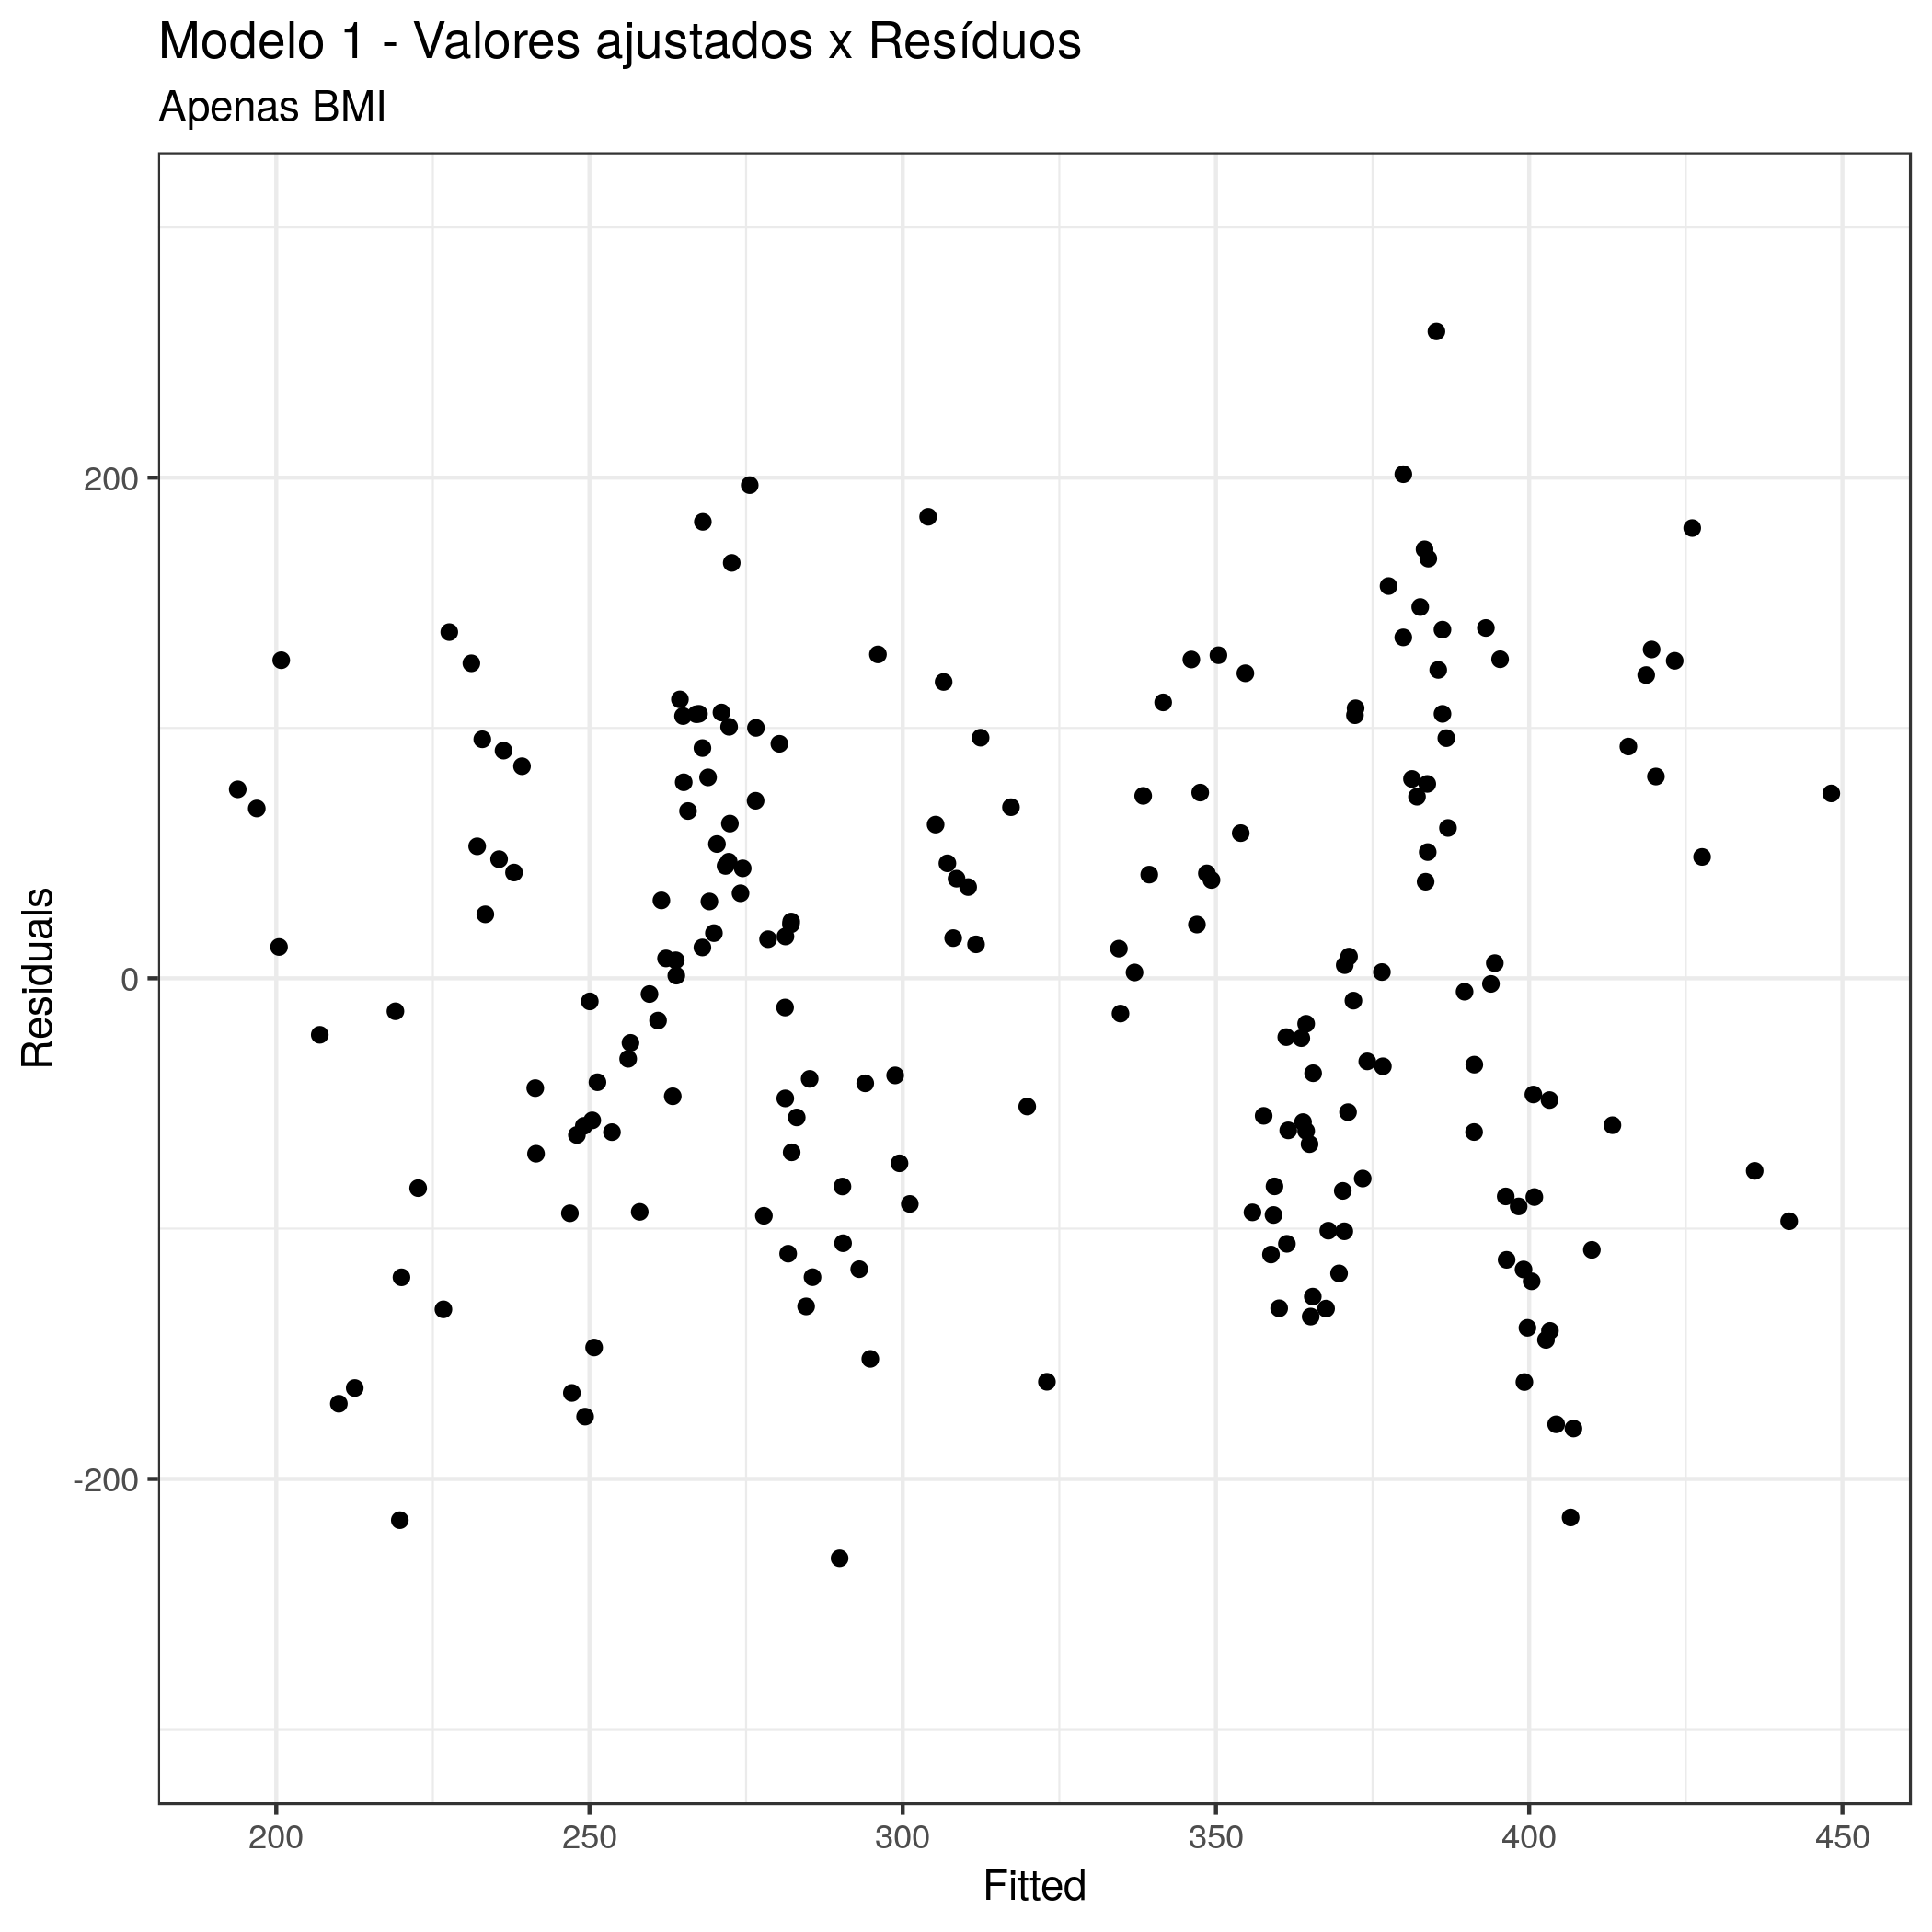
\includegraphics[height=.6\textheight]{Cap31-32/pratica-rlm1-resid}
    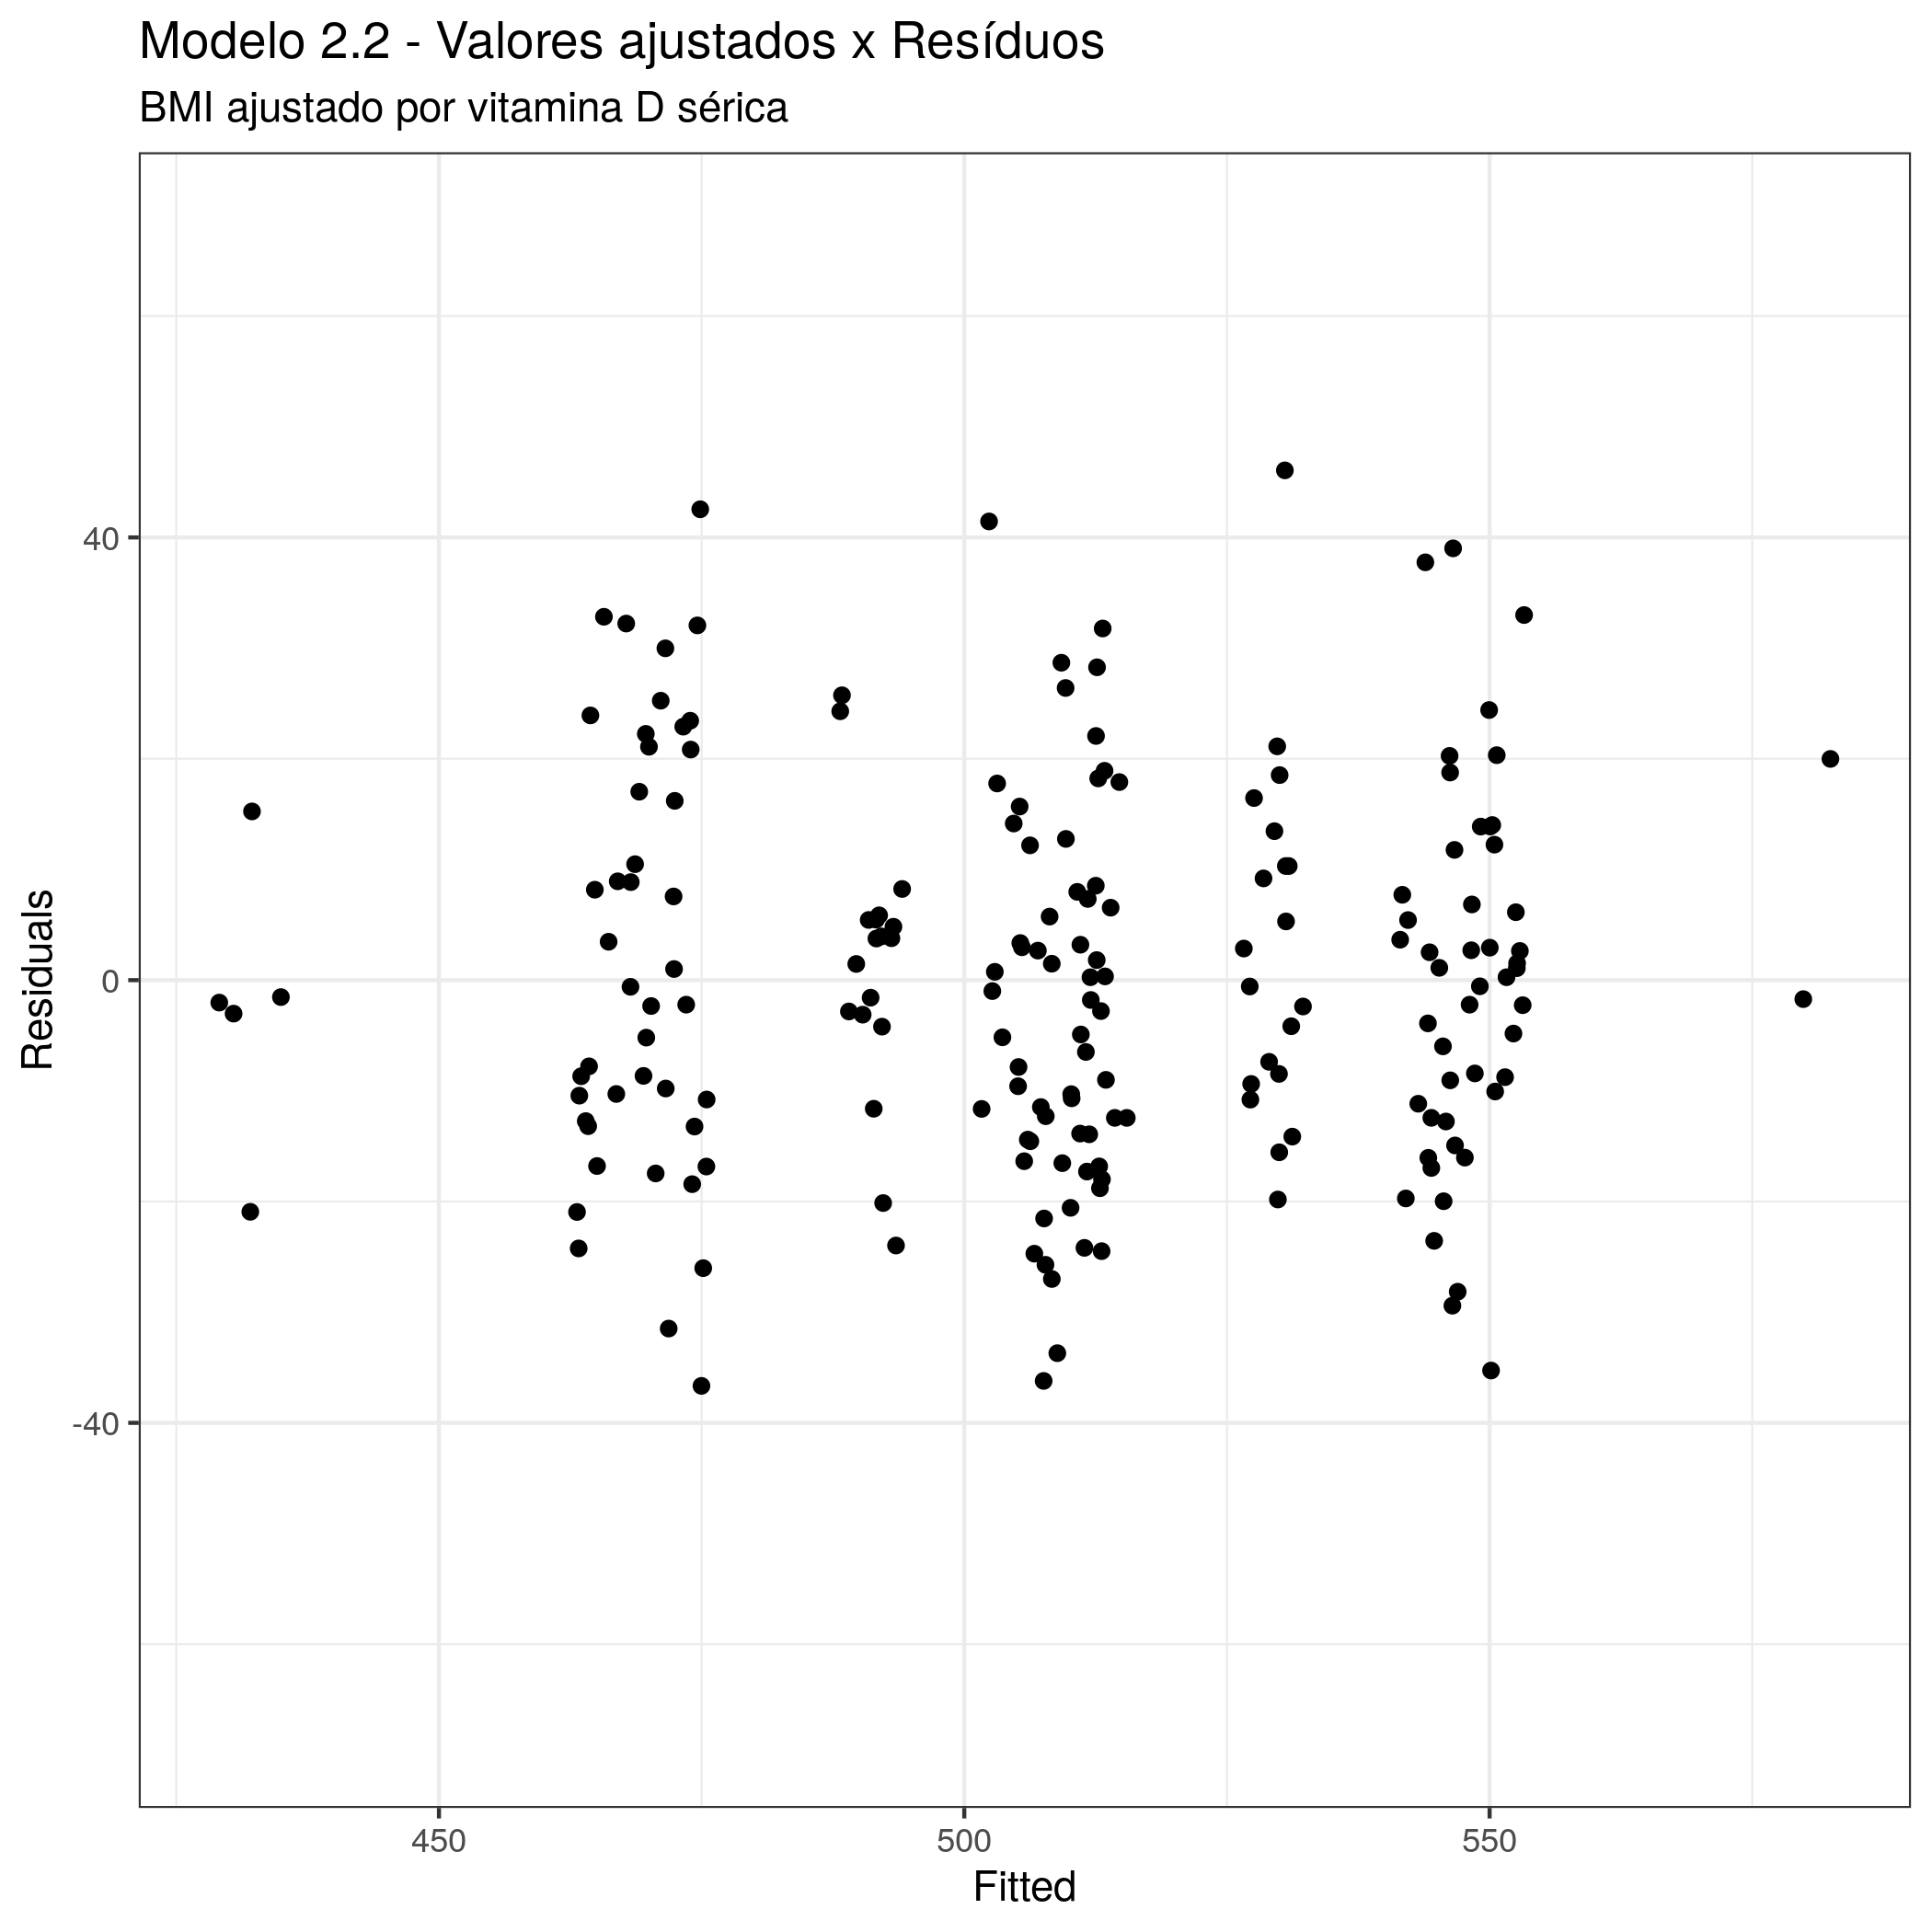
\includegraphics[height=.6\textheight]{Cap31-32/pratica-rlm2_2-resid}
  \end{center}
\end{frame}

\begin{frame}[fragile]{\scriptsize }
  \begin{center}
    \begin{exampleblock}{Modelo 2.2}
      \tiny
\begin{verbatim}
Residuals:
    Min      1Q  Median      3Q     Max 
-35.757 -12.239  -0.626  10.176  45.081 

Coefficients:
            Estimate Std. Error t value Pr(>|t|)    
(Intercept) 589.6897     5.2782 111.722  < 2e-16 ***
BMI          -1.9055     0.1187 -16.049  < 2e-16 ***
hormmedio    28.9182     2.9694   9.739  < 2e-16 ***
hormalto     17.7913     2.8720   6.195 3.37e-09 ***
---
Signif. codes:  0 ‘***’ 0.001 ‘**’ 0.01 ‘*’ 0.05 ‘.’ 0.1 ‘ ’ 1

Residual standard error: 16.98 on 196 degrees of freedom
Multiple R-squared:  0.6595,	Adjusted R-squared:  0.6543 
F-statistic: 126.6 on 3 and 196 DF,  p-value: < 2.2e-16
\end{verbatim}
    \end{exampleblock}
  \end{center}
\end{frame}

\begin{frame}{\scriptsize }
  \begin{block}{}
    \footnotesize
    As participantes perdem, na média, 1.98 unidades de BMD para cada incremento unitário do BMI (resultado bruto).

    \bigskip
    Após ajustar pelo hormônio, o resultado é 1.90.
  \end{block}
\end{frame}

% \begin{frame}{\scriptsize Quais são as variáveis?}
%   \begin{itemize}
%   \item Dependente: BMD (contínua)
%   \item Independente: BMI (contínua)
%   \item Independente: idade (contínua)
%   \item Independente: hormônio (categórica -- 3 níveis)
%   \end{itemize}
%   \vfill
%   \begin{block}{Esta relação pode ser expressa como}
%     \begin{displaymath}
%       \text{BMD} \sim \text{BMI} + \text{idade} +\text{hormônio}
%     \end{displaymath}
%   \end{block}
% \end{frame}

\begin{frame}{\scriptsize }
  \begin{center}
    Agora um modelo maior (ajustando para todas as variáveis relevantes)
  \end{center}
\end{frame}

\begin{frame}{\scriptsize Componentes do modelo 3}
  \begin{block}{\footnotesize Versão simplificada (apenas variáveis)}
    \footnotesize
    \begin{displaymath}
      \text{BMD} \sim \text{BMI} + \text{idade} + \text{hormônio}
    \end{displaymath}
  \end{block}
  \bigskip
  \bigskip
  \begin{block}{Modelo completo}
    \footnotesize
    \begin{displaymath}
      \text{BMD} =\beta_0 + \beta_1 \text{(BMI)} + \beta_2 \text{(idade)} + \beta_3 \text{(hormônio)} +\varepsilon
    \end{displaymath}
  \end{block}
  \vfill
  % \footnotesize
  % Hipótese: $\varepsilon$ é um erro aleatório \footnote{\scriptsize residual -- não é explicado pela relação entre as variáveis do modelo} normalmente distribuído e centrado em zero -- a incerteza que não pode ser controlada.
\end{frame}

\begin{frame}[fragile]{\scriptsize }
  \begin{center}
    \begin{exampleblock}{Modelo 3}
      \tiny
\begin{verbatim}
Residuals:
     Min       1Q   Median       3Q      Max 
-18.3964  -4.1337  -0.5398   4.4640  25.6025 

Coefficients:
             Estimate Std. Error t value Pr(>|t|)    
(Intercept) 774.02125    6.48702  119.32   <2e-16 ***
BMI          -1.94720    0.04992  -39.00   <2e-16 ***
idade        -3.02783    0.10013  -30.24   <2e-16 ***
hormmedio    29.35318    1.24821   23.52   <2e-16 ***
hormalto     16.32422    1.20813   13.51   <2e-16 ***
---
Signif. codes:  0 ‘***’ 0.001 ‘**’ 0.01 ‘*’ 0.05 ‘.’ 0.1 ‘ ’ 1

Residual standard error: 7.139 on 195 degrees of freedom
Multiple R-squared:  0.9402,	Adjusted R-squared:  0.9389 
F-statistic: 765.9 on 4 and 195 DF,  p-value: < 2.2e-16
\end{verbatim}
    \end{exampleblock}
  \end{center}
\end{frame}

\begin{frame}{\scriptsize Modelo 3}
  \begin{center}
    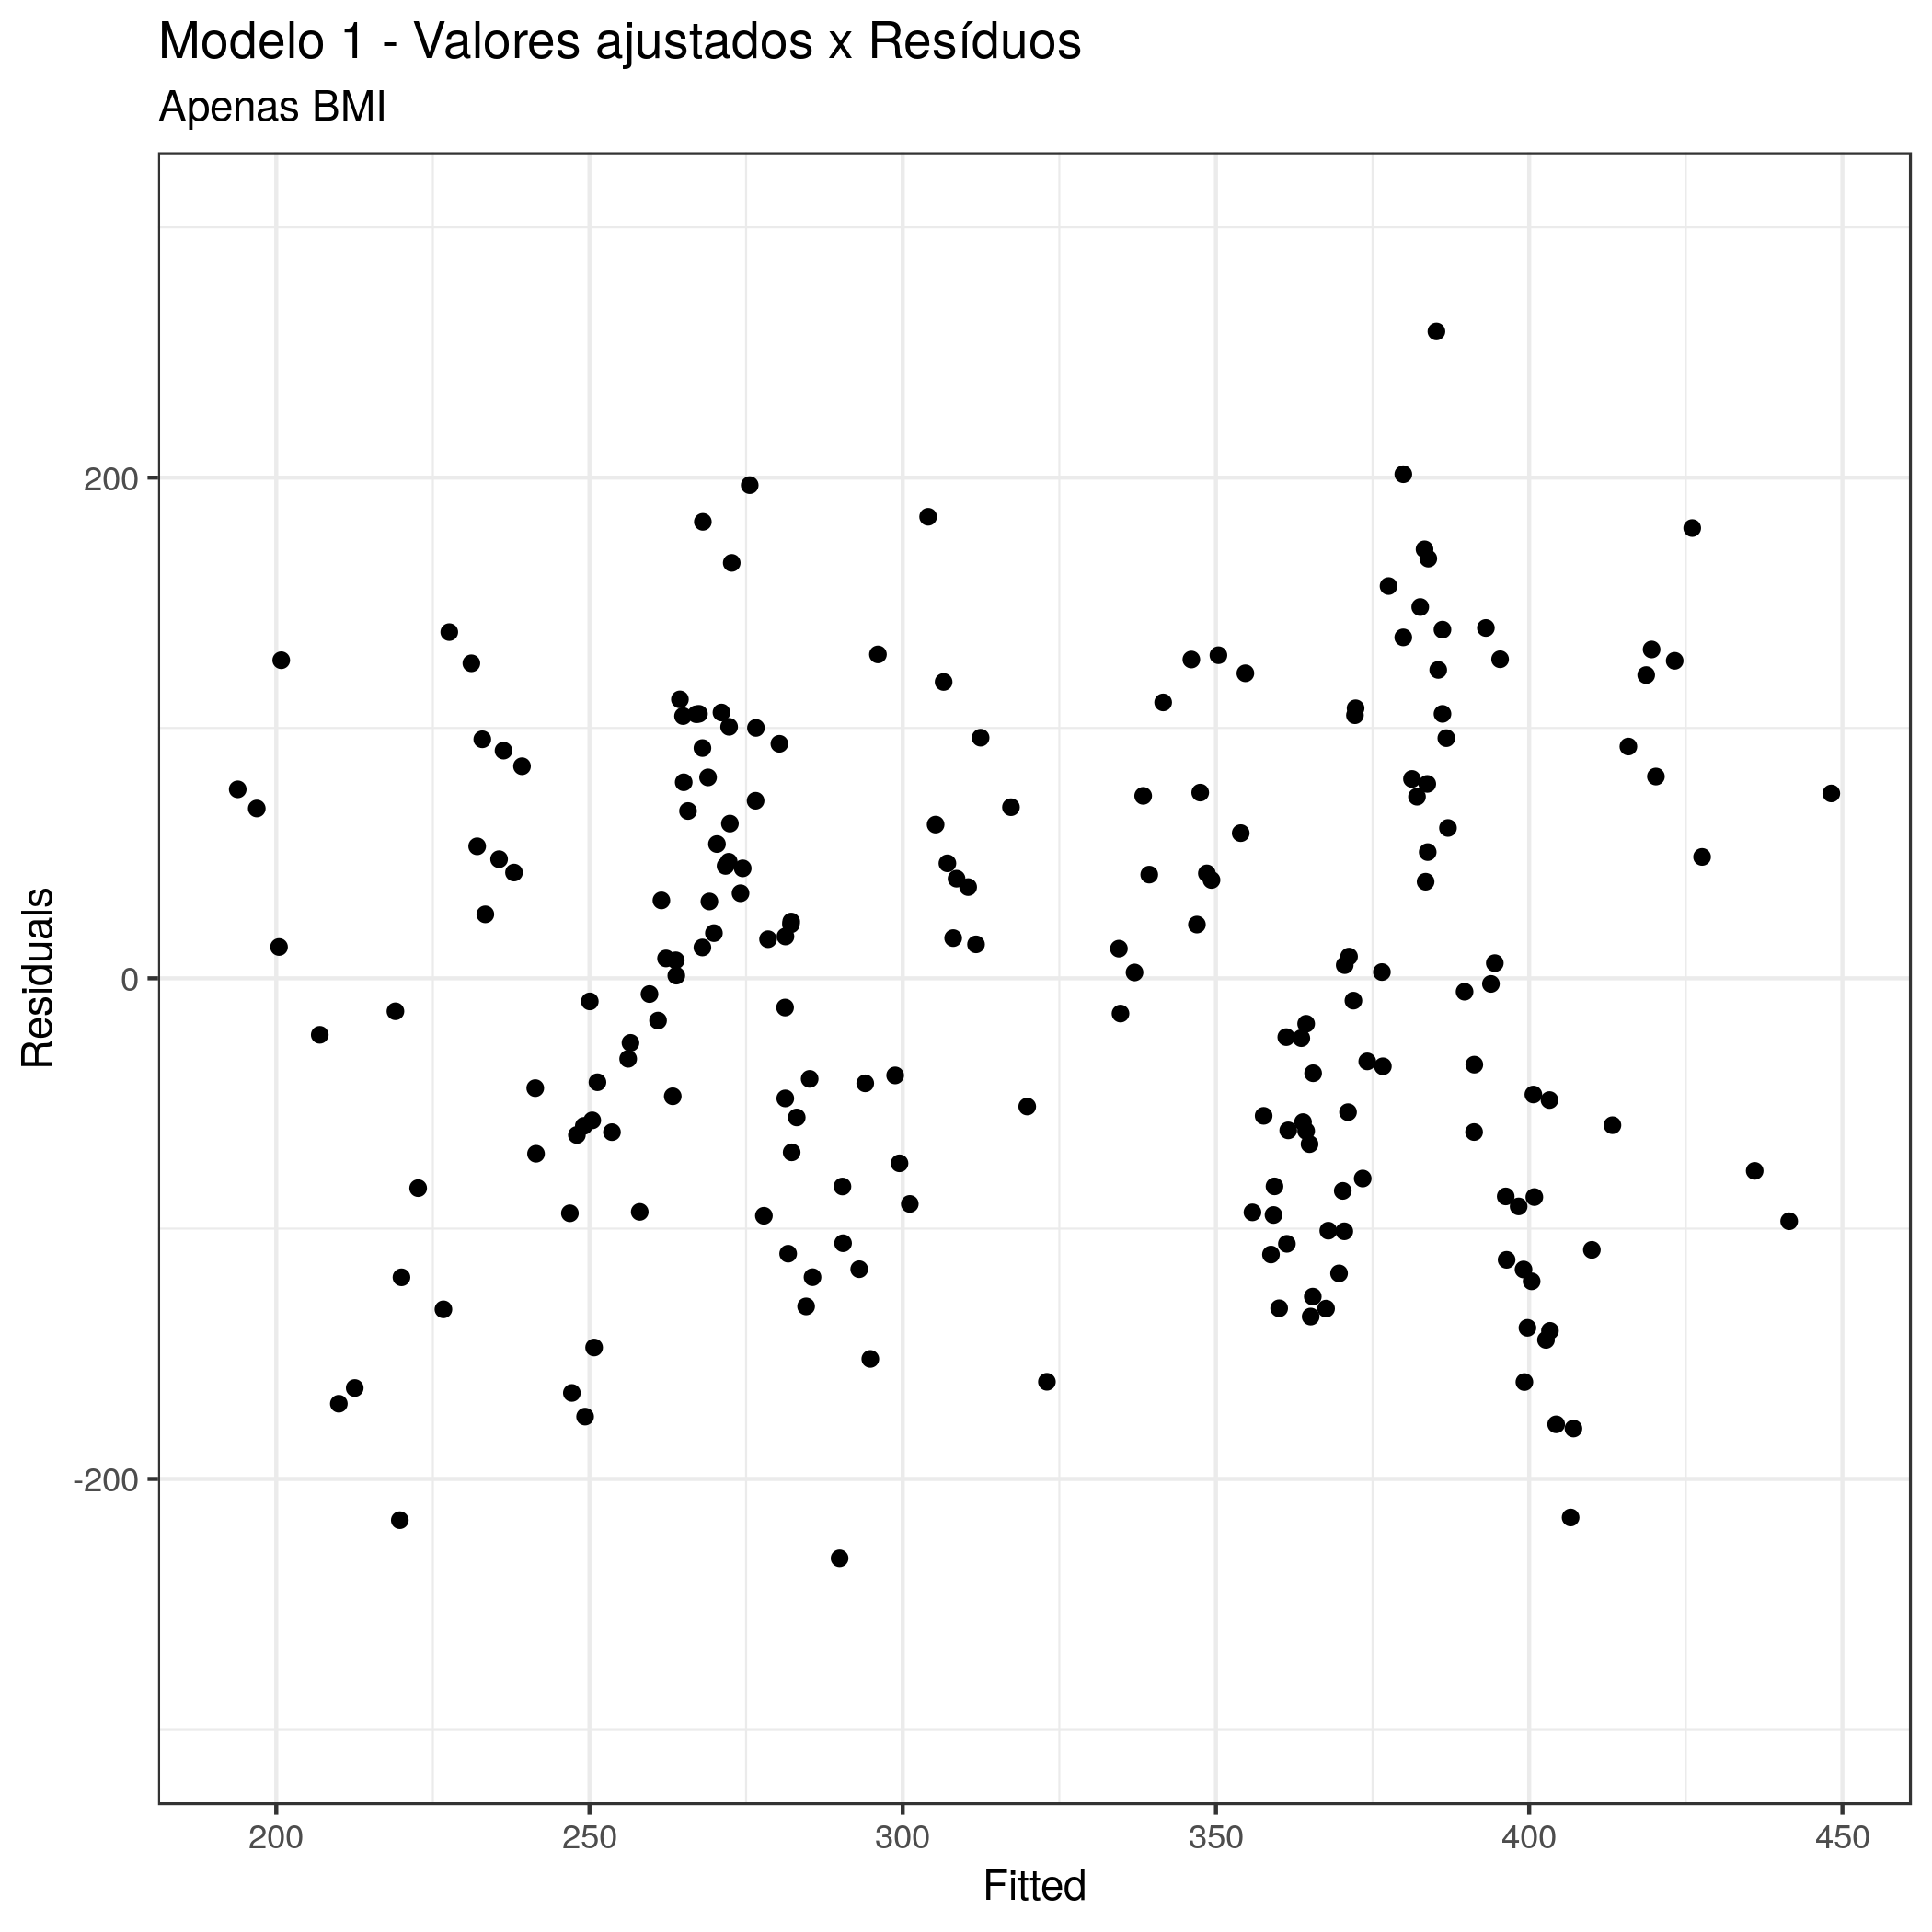
\includegraphics[height=.6\textheight]{Cap31-32/pratica-rlm1-resid}
    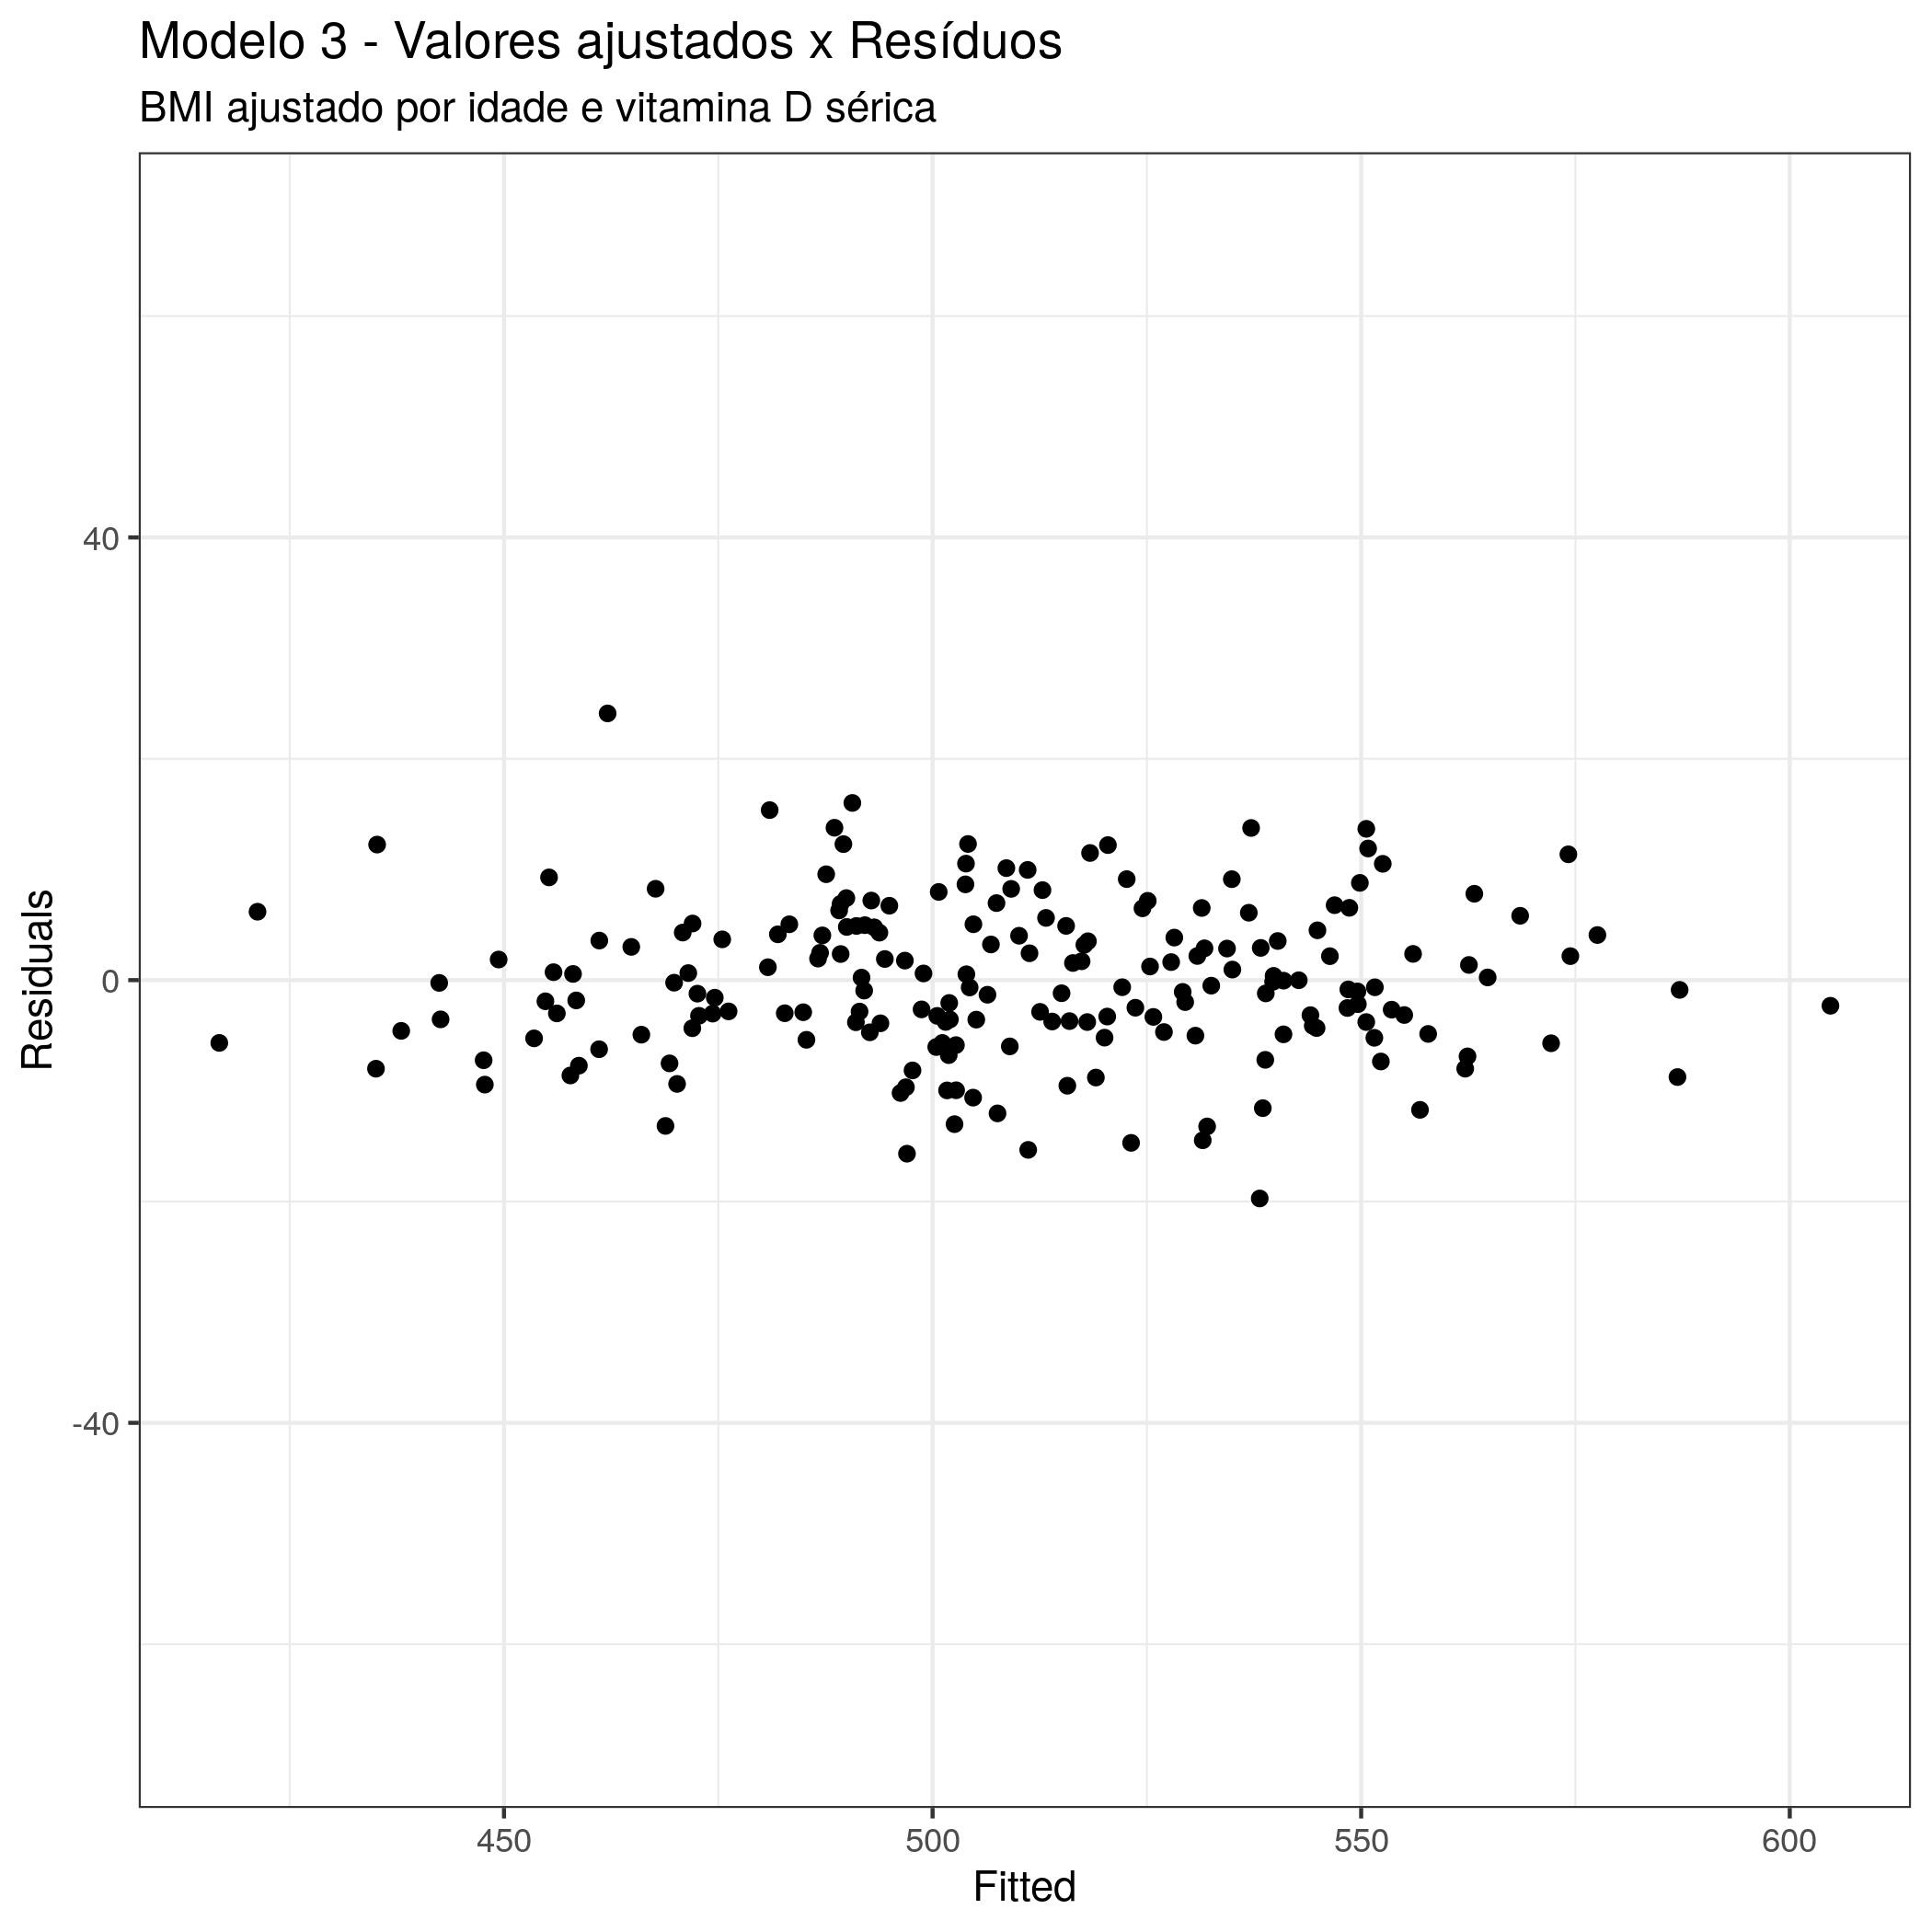
\includegraphics[height=.6\textheight]{Cap31-32/pratica-rlm3-resid}
  \end{center}
\end{frame}

\begin{frame}{\scriptsize }
  \begin{block}{}
    \footnotesize
    As participantes perdem, na média, 1.98 unidades de BMD para cada incremento unitário do BMI (resultado bruto).

    \bigskip
    Após ajustar pela idade e pelo hormônio, o resultado é 1.95.
  \end{block}
\end{frame}

\section{Regressão Logística}

\subsection{Regressão Logística}

\begin{frame}{\scriptsize Modelo 4}
  \begin{center}
    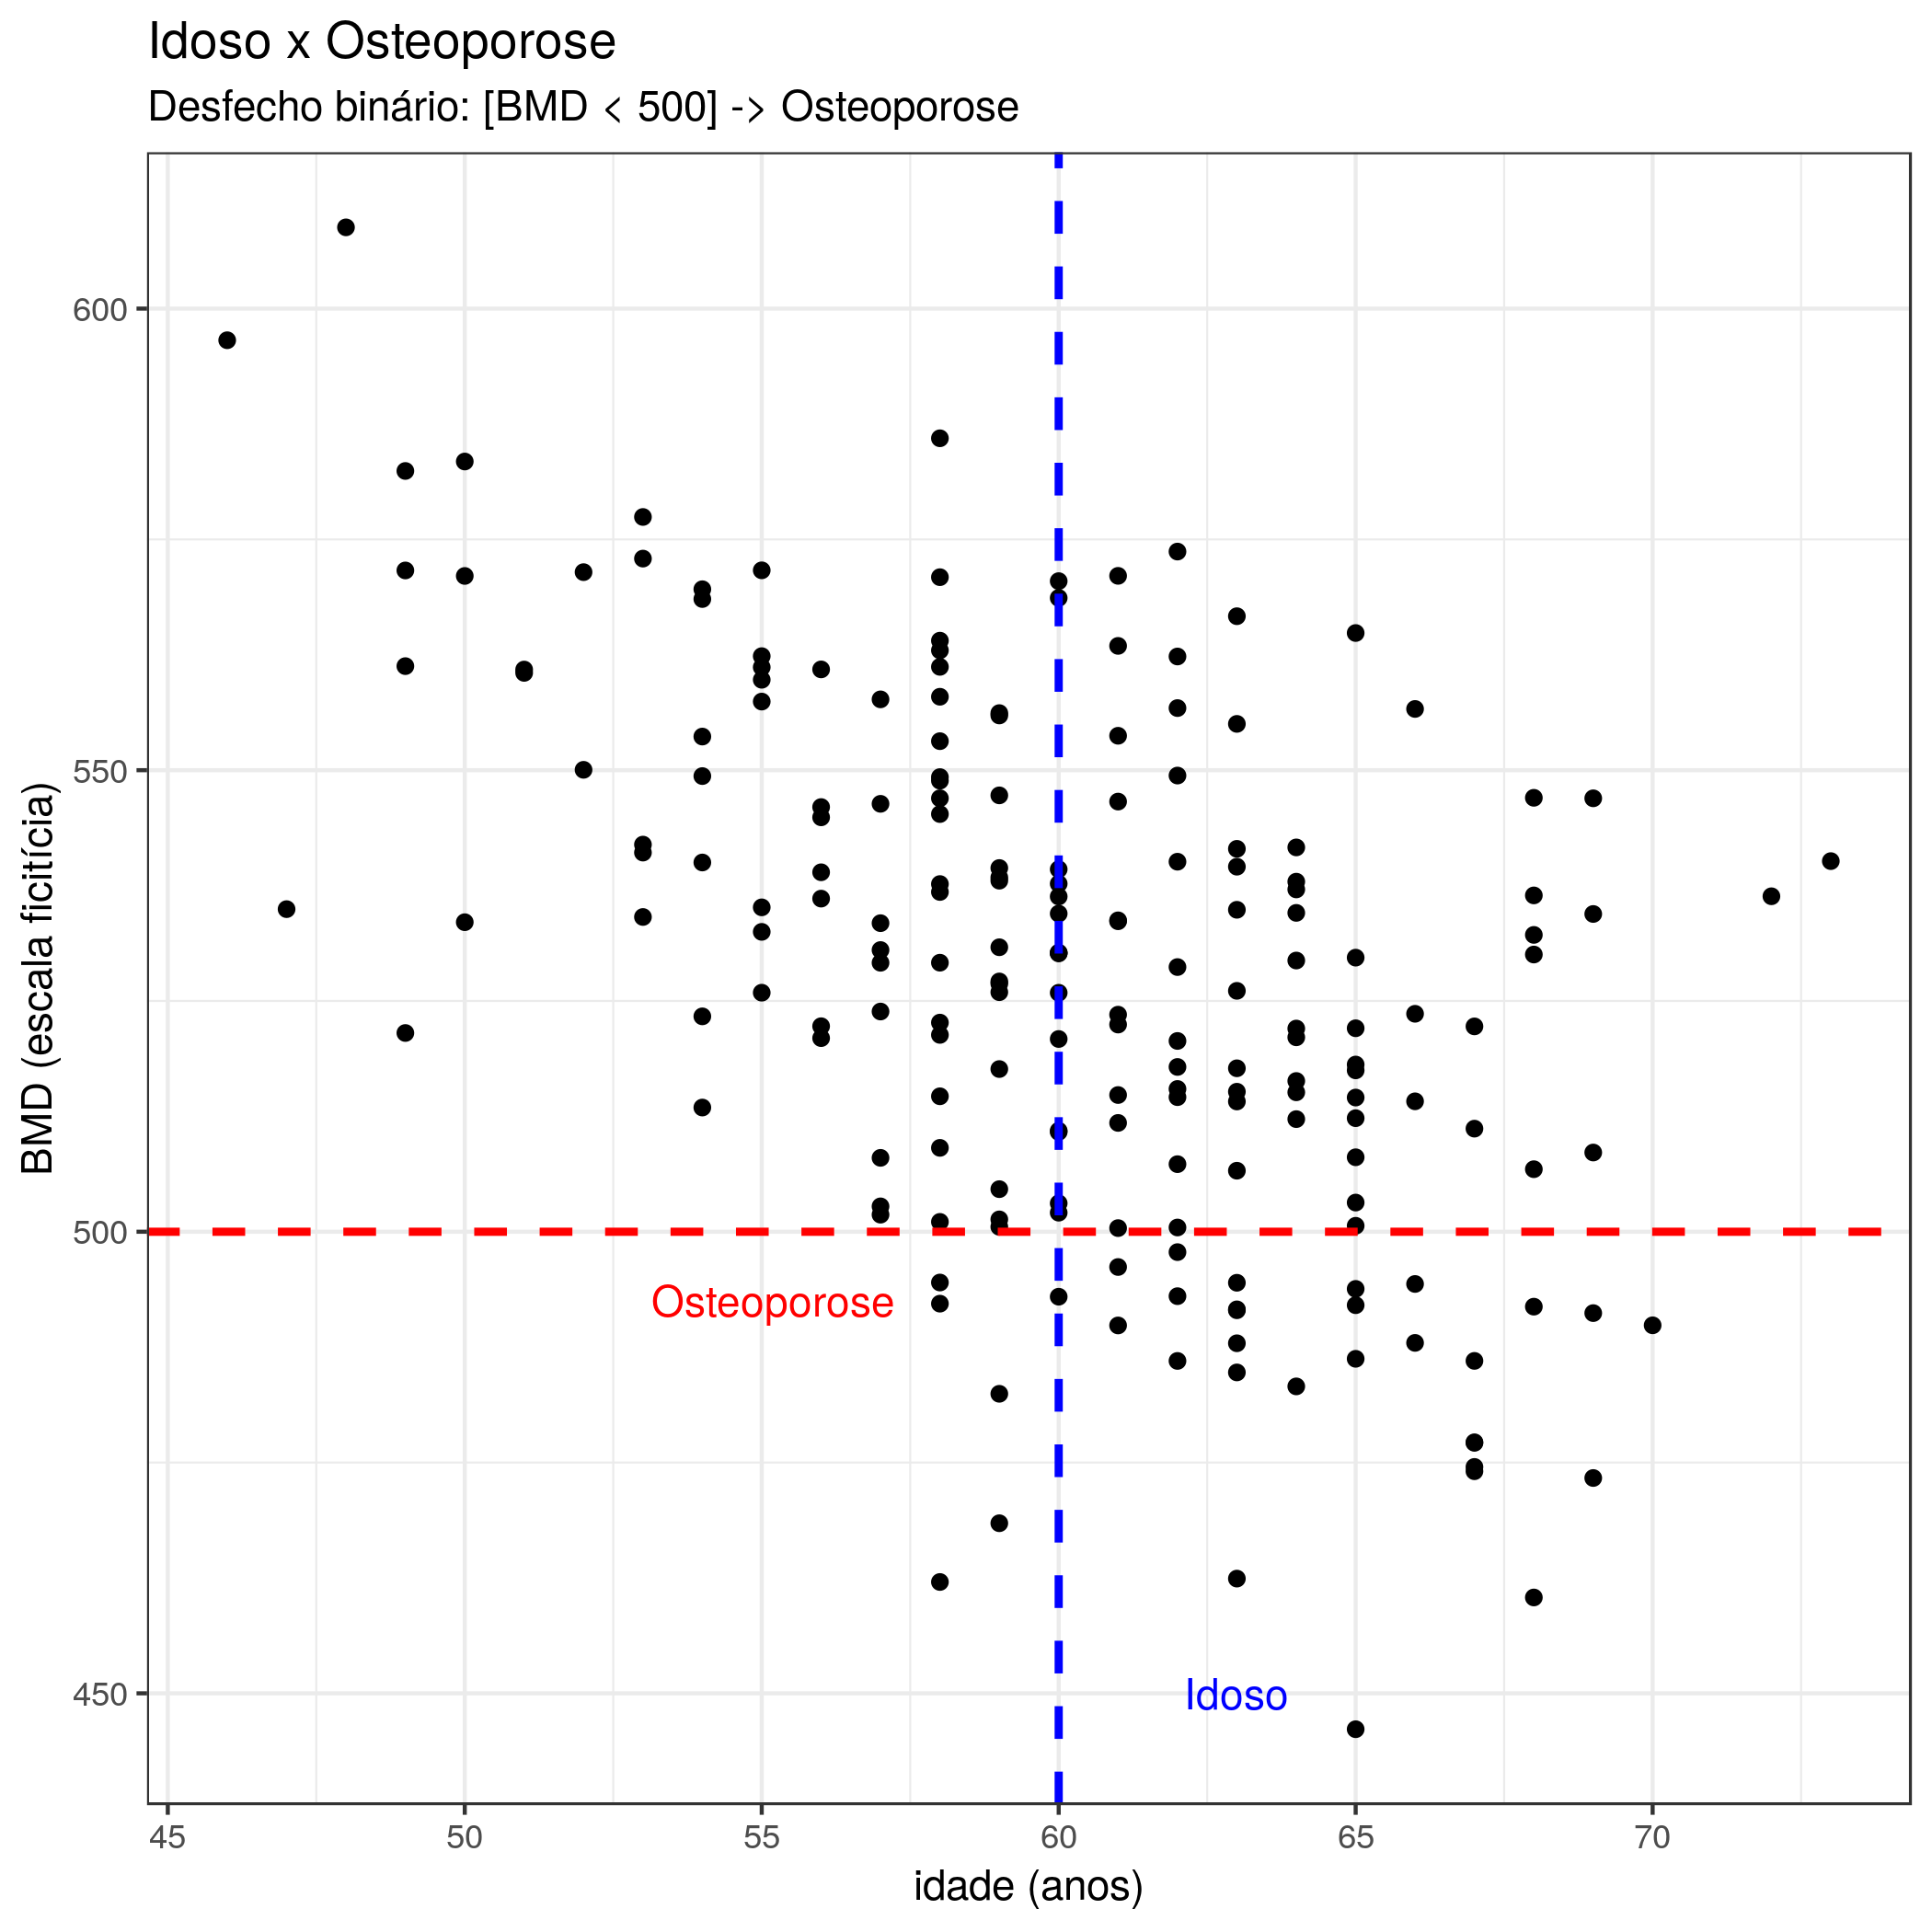
\includegraphics[height=.9\textheight]{Cap31-32/pratica-glm4}
  \end{center}
\end{frame}

\begin{frame}{\scriptsize Quais são as variáveis?}
  \begin{itemize}
    \footnotesize
  \item \alert{Dependente: Osteoporose (categórica -- binária)}
  \item Independente: Idoso (categórica -- binária)
  \end{itemize}
  \vfill
  \begin{block}{Esta relação pode ser expressa como}
    \footnotesize
    \begin{displaymath}
      \text{Osteoporose} \sim \text{Idoso}
    \end{displaymath}
  \end{block}
\end{frame}

\begin{frame}{\scriptsize Componentes do modelo 4}
  \begin{block}{\footnotesize Versão simplificada (apenas variáveis)}
    \footnotesize
    \begin{displaymath}
      \text{Osteoporose} \sim \text{Idoso}
    \end{displaymath}
  \end{block}
  \bigskip
  \bigskip
  \begin{block}{Modelo completo}
    \footnotesize
    \begin{displaymath}
      \text{Osteoporose} =\beta_0 + \beta_1 \text{(Idoso)} +\varepsilon
    \end{displaymath}
  \end{block}
  \vfill
  % \footnotesize
  % Hipótese: $\varepsilon$ é um erro aleatório \footnote{\scriptsize residual -- não é explicado pela relação entre as variáveis do modelo} normalmente distribuído e centrado em zero -- a incerteza que não pode ser controlada.
\end{frame}

\begin{frame}[fragile]{\scriptsize }
  \begin{exampleblock}{\small Tabela de contingência Idoso x Osteoporose}
    \tiny
\begin{verbatim}
           osteo
idoso       Sadio Osteoporose
  Nao Idoso    98           6
  Idoso        68          28
\end{verbatim}
  \end{exampleblock}
  \begin{center}
    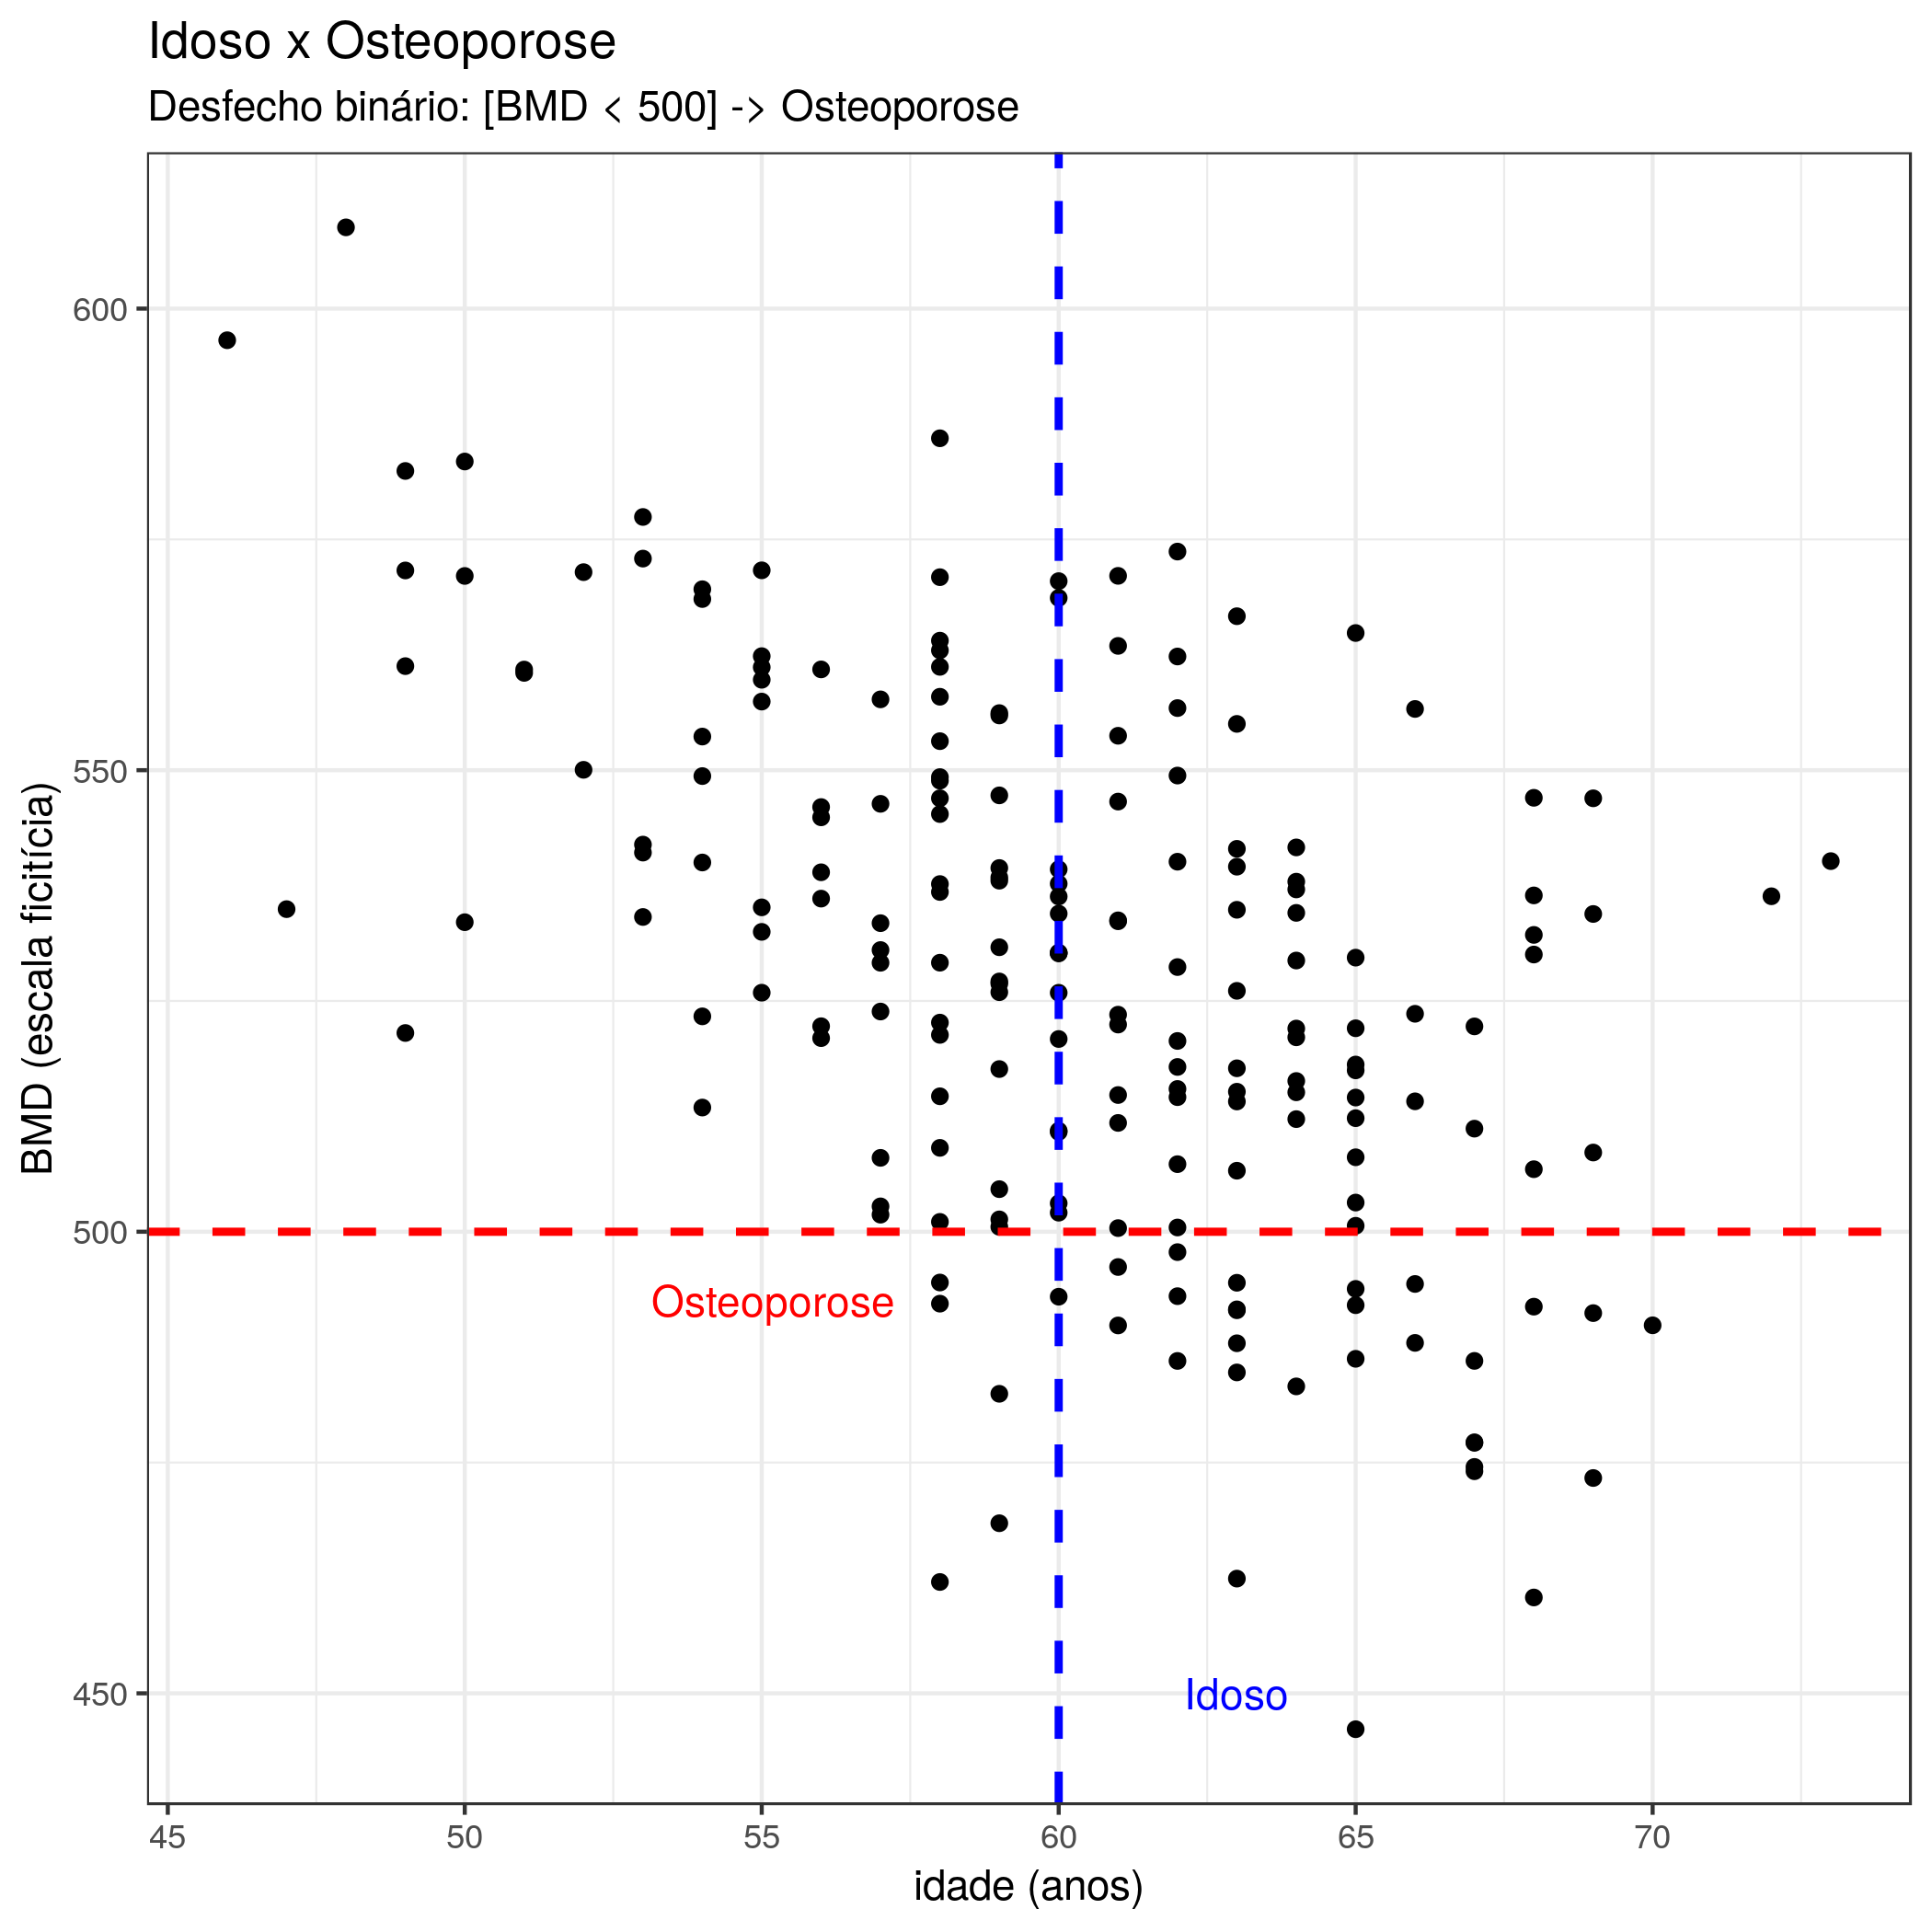
\includegraphics[height=.6\textheight]{Cap31-32/pratica-glm4}
  \end{center}
%   \begin{exampleblock}{\small Razão de chance Idoso x Osteoporose}<2->
%     \tiny
% \begin{verbatim}
% 	Fisher's Exact Test for Count Data

% data:  tc.idoso.osteo
% p-value = 0.0001001
% alternative hypothesis: true odds ratio is not equal to 1
% 95 percent confidence interval:
%     3.94893 1619.54319
% sample estimates:
% odds ratio 
%   34.36342 
% \end{verbatim}
%   \end{exampleblock}
%   \begin{block}{\small OR}<2->
%     \begin{center}
%       OR $\approx 34$
%     \end{center}
%   \end{block}
\end{frame}

\begin{frame}[fragile]{\scriptsize }
  \begin{center}
    \begin{exampleblock}{Modelo 4}
      \tiny
\begin{verbatim}
Deviance Residuals: 
    Min       1Q   Median       3Q      Max  
-0.8305  -0.8305  -0.3447  -0.3447   2.3886  

Coefficients:
            Estimate Std. Error z value Pr(>|z|)    
(Intercept)  -2.7932     0.4206  -6.642 3.10e-11 ***
idosoIdoso    1.9059     0.4767   3.998 6.39e-05 ***
---
Signif. codes:  0 ‘***’ 0.001 ‘**’ 0.01 ‘*’ 0.05 ‘.’ 0.1 ‘ ’ 1

(Dispersion parameter for binomial family taken to be 1)

    Null deviance: 182.35  on 199  degrees of freedom
Residual deviance: 161.78  on 198  degrees of freedom
AIC: 165.78

Number of Fisher Scoring iterations: 5
\end{verbatim}
    \end{exampleblock}
    \begin{block}{\small log da OR de um idoso x osteoporose}<2->
    \footnotesize
      $$\log \left(\text{OR} \right) = 1.9059$$
    \end{block}
  \end{center}
\end{frame}

\begin{frame}{\scriptsize }
  \begin{block}{\small Transformando o log da OR na OR }
    \footnotesize
    $$\log \left(\text{OR} \right) \approx 1.90...$$
    \begin{center}
      \small
      ... portanto...
    \end{center}
    \footnotesize
    $$e^{1.90} \approx 6.7$$
  \end{block}

  \bigskip
  \bigskip
  \begin{block}{Resultado}<2->
    \footnotesize
    \begin{itemize}
    \footnotesize
    \item (Idoso) {\bf OR: 6.73, IC: [2.64, 17.12]}
    \end{itemize}
  \end{block}
\end{frame}

\begin{frame}{\scriptsize Modelo 5}
  \begin{center}
    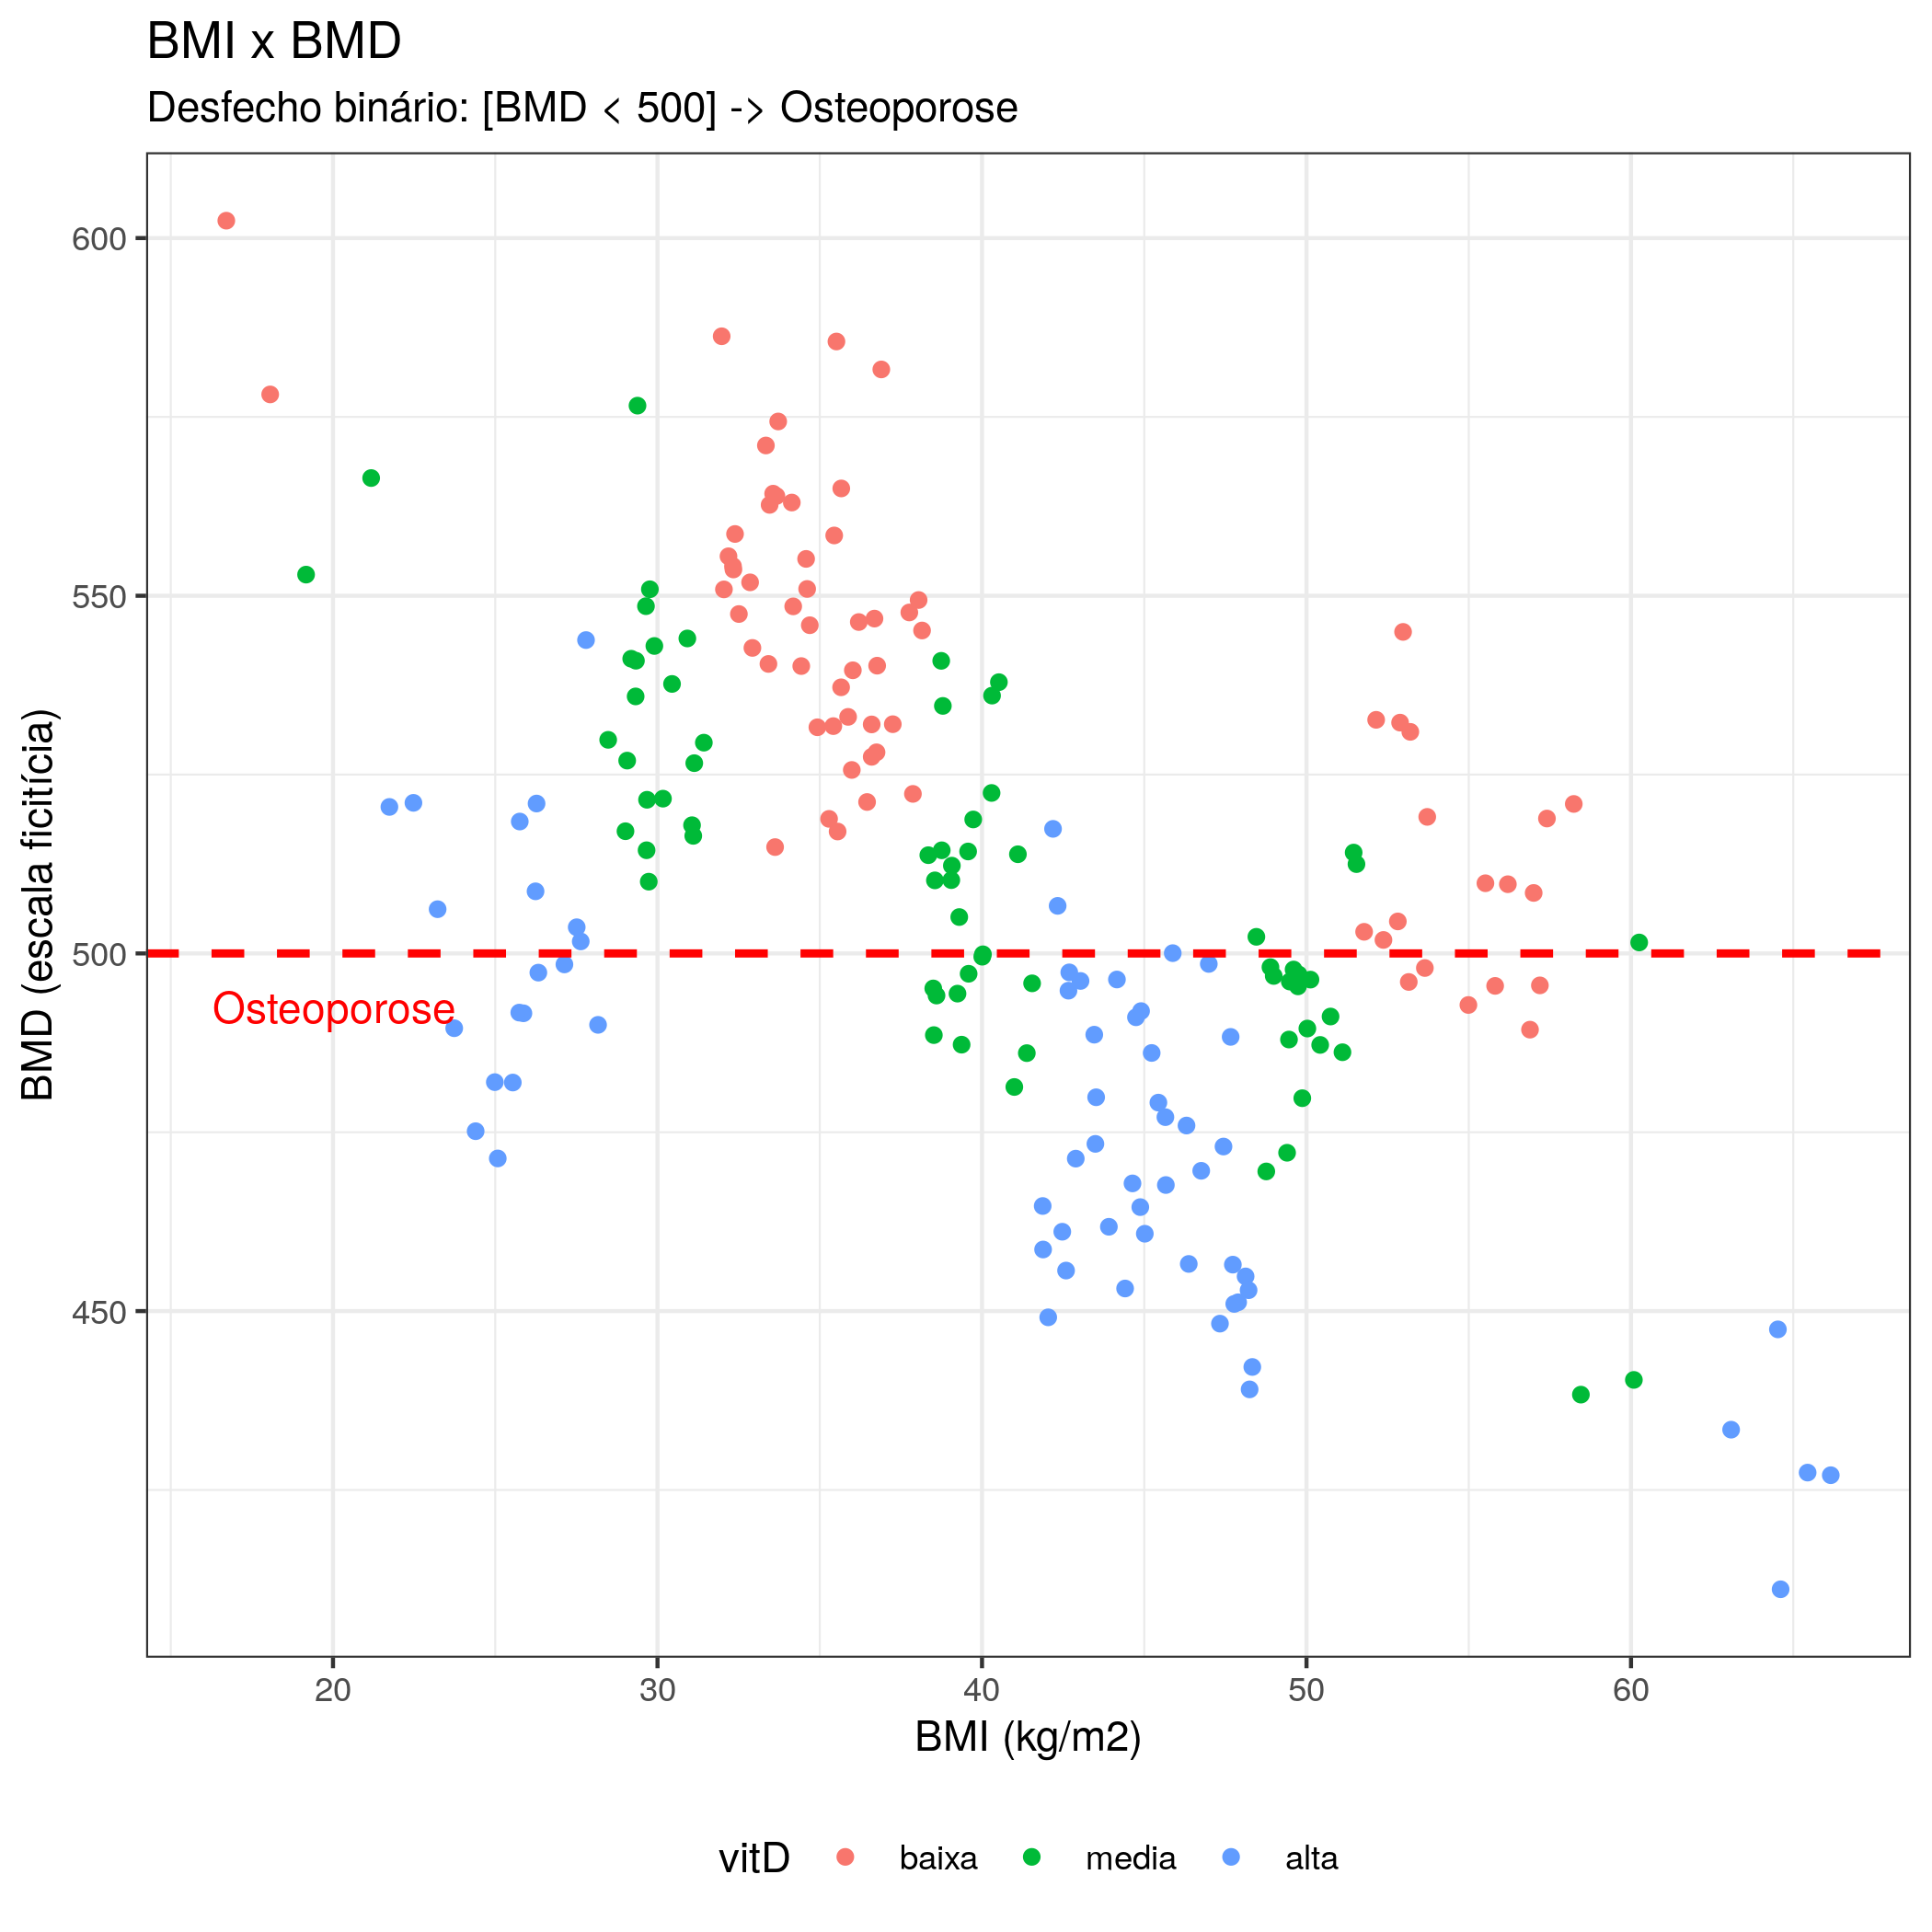
\includegraphics[height=.9\textheight]{Cap31-32/pratica-glm5}
  \end{center}
\end{frame}

\begin{frame}{\scriptsize Quais são as variáveis?}
  \begin{itemize}
    \footnotesize
  \item \alert{Dependente: Osteoporose (categórica -- binária)}
  \item Independente: BMI (contínua)
  \item Independente: idade (contínua)
  \item Independente: hormônio (categórica -- 3 níveis)
  \end{itemize}
  \vfill
  \begin{block}{Esta relação pode ser expressa como}
    \footnotesize
    \begin{displaymath}
      \text{Osteoporose} \sim \text{BMI} + \text{idade} +\text{hormônio}
    \end{displaymath}
  \end{block}
\end{frame}

\begin{frame}{\scriptsize Componentes do modelo 5}
  \begin{block}{\footnotesize Versão simplificada (apenas variáveis)}
    \footnotesize
    \begin{displaymath}
      \text{Osteoporose} \sim \text{BMI} + \text{idade} + \text{hormônio}
    \end{displaymath}
  \end{block}
  \bigskip
  \bigskip
  \begin{block}{Modelo completo}
    \footnotesize
    \begin{displaymath}
      \text{Osteoporose} =\beta_0 + \beta_1 \text{(BMI)} + \beta_2 \text{(idade)} + \beta_3 \text{(hormônio)} +\varepsilon
    \end{displaymath}
  \end{block}
  \vfill
  % \footnotesize
  % Hipótese: $\varepsilon$ é um erro aleatório \footnote{\scriptsize residual -- não é explicado pela relação entre as variáveis do modelo} normalmente distribuído e centrado em zero -- a incerteza que não pode ser controlada.
\end{frame}

\begin{frame}[fragile]{\scriptsize }
  \begin{center}
    \begin{exampleblock}{Modelo 5}
      \tiny
\begin{verbatim}
Deviance Residuals: 
     Min        1Q    Median        3Q       Max  
-1.85523  -0.08866  -0.01263  -0.00068   2.05724  

Coefficients:
            Estimate Std. Error z value Pr(>|z|)    
(Intercept) -77.4340    18.0040  -4.301 1.70e-05 ***
BMI           0.4554     0.1089   4.183 2.88e-05 ***
idade         0.8285     0.2086   3.972 7.13e-05 ***
hormmedio     1.9614     1.4716   1.333 0.182590    
hormalto      5.5205     1.5101   3.656 0.000257 ***
---
Signif. codes:  0 ‘***’ 0.001 ‘**’ 0.01 ‘*’ 0.05 ‘.’ 0.1 ‘ ’ 1

(Dispersion parameter for binomial family taken to be 1)

    Null deviance: 182.354  on 199  degrees of freedom
Residual deviance:  43.436  on 195  degrees of freedom
AIC: 53.436

Number of Fisher Scoring iterations: 9
\end{verbatim}
    \end{exampleblock}
  \end{center}
\end{frame}

\begin{frame}{\scriptsize }
  \begin{block}{Resultado}
    \footnotesize
    \begin{itemize}
      \scriptsize
    \item {\small (BMI)} {\bf OR: 1.58, IC: [1.27, 1.95]}
      \medskip
    \item {\small (idade)} {\bf OR: 2.29, IC: [1.52, 3.45]}
      \medskip
    \item {\small (hormônio médio x baixo)} {\bf OR: 7.11, IC: [0.40, 127.19]}
      \medskip
    \item {\small (hormônio alto x baixo)} {\bf OR: 249.76, IC: [12.94, 4818.87]}
    \end{itemize}
  \end{block}
    \begin{block}{Interpretação}
    \footnotesize
    Após ajustar pela idade e pelo hormônio, as participantes tem chance aumentada de desenvolver osteoporose para cada incremento unitário do BMI.
  \end{block}
\end{frame}

\section{Aprofundamento}

\subsection{Aprofundamento}

\begin{frame}{\scriptsize Aprofundamento}
  \begin{block}{Leitura obrigatória}
    \begin{itemize}
      \footnotesize
    \item Capítulo 31
    \item Capítulo 32
    \end{itemize}
  \end{block}
  \begin{block}{Leitura recomendada}
    \scriptsize
    Capítulo 25: seção teste t de uma razão ({\tiny sobre o uso do logaritmo})

    % \begin{itemize}

    % \end{itemize}
  \end{block}
\end{frame}


\end{document}
